\documentclass[a4paper, 10pt, titlepage, twoside]{report}
\usepackage[a4paper]{geometry}
\usepackage{fancyhdr}
\usepackage{charter}
\usepackage[british]{babel}
\usepackage{pstricks,pst-node,pst-text,pst-3d,pst-eucl}
\usepackage{psfrag}
\usepackage{import}
\usepackage{graphicx}
\usepackage{subfigure}
\usepackage[figuresright]{rotating}
\usepackage{amssymb,amstext,amsfonts} %% ... with default font
\usepackage{amsmath}
\usepackage{mathrsfs}
%\usepackage{txfonts}
\usepackage{listings}
\usepackage{enumitem}
\usepackage{booktabs, longtable, dcolumn}
\usepackage[labelfont=bf]{caption}
\usepackage[caption2]{ccaption}
%\usepackage{tikz}
%\usetikzlibrary{shapes,arrows}
\usepackage{lmodern}
\renewcommand{\sfdefault}{lmss}
\renewcommand{\ttdefault}{lmtt}
\usepackage{microtype}
\usepackage[T1]{fontenc}
\usepackage{braket}
\usepackage{slashed}
\usepackage{afterpage}
\usepackage{appendix}
\usepackage[latin9]{inputenc}
%\usepackage{fixmath}
\usepackage{ upgreek }
%\usepackage{paralist}
\usepackage{hyperref}
\usepackage[authoryear]{natbib}
\renewcommand{\bibfont}{\footnotesize}
\addto{\captionsbritish}{\renewcommand{\bibname}{{R\lowercase{eferences}}}}
%\renewcommand{\refname}{{R\lowercase{eferences}}}
\setlength{\bibhang}{0pt} 
\setlength{\bibsep}{0.5pt}

  \hyphenpenalty=2000
  \tolerance=1000
  
\headheight 13.6pt
\headsep 0.6\baselineskip
\footskip 2\baselineskip
\textheight = 55\baselineskip

\renewcommand\floatpagefraction{.9}
\renewcommand\topfraction{.9}
\renewcommand\bottomfraction{.9}
\renewcommand\textfraction{.1}
\setcounter{topnumber}{2}
\setcounter{bottomnumber}{2}
\setcounter{totalnumber}{4} 

\setcounter{secnumdepth}{5}

\def\today{\number\day\space\ifcase\month\or January\or February\or March\or April\or May\or June\or July\or August\or September\or October\or November\or December\fi\space\number\year}

\newcommand{\eqnref}[1]{equation~(\ref{eq:#1})}
\newcommand{\Eqnref}[1]{Equation~(\ref{eq:#1})}
\newcommand{\secref}[1]{section~\ref{sec:#1}}
\newcommand{\Secref}[1]{Section~\ref{sec:#1}}
\newcommand{\chapref}[1]{chapter~\ref{ch:#1}}
\newcommand{\Chapref}[1]{Chapter~\ref{ch:#1}}
\newcommand{\apref}[1]{appendix~\ref{ap:#1}}
\newcommand{\Apref}[1]{Appendix~\ref{ap:#1}}
\newcommand{\tabref}[1]{table~\ref{tab:#1}}
\newcommand{\Tabref}[1]{Table~\ref{tab:#1}}
\newcommand{\figref}[1]{figure~\ref{fig:#1}}
\newcommand{\Figref}[1]{Figure~\ref{fig:#1}}

\DeclareMathOperator{\sinc}{sinc}

\newcommand{\units}[1]{\ensuremath{~\mathrm{#1}}}

\newcommand{\sub}[1]{\ensuremath{_\mathrm{#1}}}
\newcommand{\super}[1]{\ensuremath{^\mathrm{#1}}}

\newcommand{\recip}[1]{\ensuremath{\frac{1}{#1}}}

\newcommand{\order}[1]{\ensuremath{\mathcal{O}\left({#1}\right)}}

\newcommand{\innerprod}[2]{\ensuremath{\left({#1}\middle|{#2}\right)}}

\newcommand{\Ibar}{{\declareslashed{}{\text{-}}{0.04}{-0.2}{I}\slashed{I}}}
\newcommand{\lambdabar}{{\declareslashed{}{\text{--}}{0.04}{-0.02}{\lambda}\slashed{\lambda}}}

\newcommand{\upDelta}{\Delta}

% Define differential operators
\newcommand{\dd}{\ensuremath{\mathrm{d}}}
\newcommand{\diff}[2]{\ensuremath{\frac{\dd {#1}}{\dd {#2}}}}
\newcommand{\linediff}[2]{\ensuremath{\dd {#1}/\dd {#2}}}
\newcommand{\diffop}[1]{\ensuremath{\frac{\dd}{\dd {#1}}}}
\newcommand{\difftwo}[2]{\ensuremath{\frac{\dd^2 {#1}}{\dd {#2}^2}}}
\newcommand{\linedifftwo}[2]{\ensuremath{\dd^2 {#1}/\dd {#2}^2}}
\newcommand{\difftwoop}[1]{\ensuremath{\frac{\dd^2}{\dd {#1}^2}}}
\newcommand{\diffn}[3]{\ensuremath{\frac{\dd^{#3} {#1}}{\dd {#2}^{#3}}}}
\newcommand{\linediffn}[3]{\ensuremath{\dd^{#3} {#1}/\dd {#2}^{#3}}}
\newcommand{\diffnop}[2]{\ensuremath{\frac{\dd^{#2}}{\dd {#1}^{#2}}}}
\newcommand{\partialdiff}[2]{\ensuremath{\frac{\partial {#1}}{\partial {#2}}}}
\newcommand{\linepartialdiff}[2]{\ensuremath{\partial {#1}/\partial {#2}}}
\newcommand{\partialdiffop}[1]{\ensuremath{\frac{\partial}{\partial {#1}}}}
\newcommand{\grad}{\ensuremath{\boldsymbol{\nabla}}}
\newcommand{\intd}[4]{\ensuremath{\int_{#1}^{#2}{#3}\,\dd{#4}}}

\begin{document}

%\bibpunct{[}{]}{,\,}{s}{}{}
\bibpunct{(}{)}{;}{a}{}{,\,}

\pagestyle{fancy}
\renewcommand{\chaptermark}[1]{
\markboth{\chaptername
\ \thechapter.\ #1}{}}
\renewcommand{\sectionmark}[1]{\markright{\thesection\ #1}}
\fancyhf{}
\fancyhead[LE]{\leftmark}
\fancyhead[RE]{Christopher Berry}
\fancyhead[LO]{Exploring Gravity}
\fancyhead[RO]{\rightmark}
\fancyfoot{}
\renewcommand{\footrulewidth}{0.1ex}
\fancyfoot[LO]{\today}
\fancyfoot[RE]{Institute of Astronomy}
\fancyfoot[RO, LE]{\thepage}
\fancypagestyle{plain}{
\fancyhf{}
\renewcommand{\headrulewidth}{0pt}
\fancyfoot{}
\renewcommand{\footrulewidth}{0.1ex}
\fancyfoot[LO]{\today}
\fancyfoot[RE]{Institute of Astronomy}
\fancyfoot[RO, LE]{\thepage}}
\renewcommand\floatpagefraction{.6}
\renewcommand\topfraction{.8}
\renewcommand\bottomfraction{.8}
\renewcommand\textfraction{.2}

\title{{\sc{}{\Huge{}Exploring Gravity}\\\vspace{1mm}{\LARGE{}with Gravitational Waves\\\& Strong-Field Tests}}}
\author{{\Large{}Christopher P.\ L.\ Berry}\vspace{3mm}\\Churchill College\vspace{0.5mm}\\and\vspace{0.5mm}\\Institute of Astronomy,\vspace{0.5mm}\\University of Cambridge\vspace{5mm}}
\date{\includegraphics[width=0.25\textwidth]{../shield.eps}\vspace{11mm}\\{\LARGE{}Ph.D.\ Thesis}\vspace{3mm}\\{\Large{}Supervisor: Jonathan R.\ Gair}\vspace{7mm}\\{\Large\today}}
\maketitle

\part{Introduction}

\chapter{Gravitation}

\section{$f(R)$}

General relativity (GR) is a well tested theory of gravity~\cite{Will2006}; so far no evidence has been found that suggests it is not the correct classical theory of gravitation. However, there are many unanswered questions that remain regarding gravity which motivate the exploration of alternate theories: What are the true natures of dark matter and dark energy? How should we formulate a quantizable theory of gravity? What drove inflation in the early Universe?  Is GR the only theory that is consistent with current observations? Moreover, the majority of the tests that have been carried out to date have been in the weak-field, low-energy regime~\cite{Will2006, Will1993}: in the laboratory~\cite{Adelberger2009, Adelberger2003}, within the Solar System~\cite{Bertotti2003, Everitt2009} or using binary pulsars~\cite{Stairs2003}. It is not unreasonable to suppose that GR would begin to break down at higher energies.

Over the coming decade, a new avenue for testing relativity will be opened up, through the detection of gravitational waves (GWs) using the existing ground-based GW detectors, the Laser Interferometer Gravitational-Wave Observatory (LIGO)~\cite{Abramovici1992, Abbott2009}, Virgo~\cite{Accadia2010} and GEO~\cite{Willke2002, Abadie2010}, and the proposed space-based GW detector, the Laser Interferometer Space Antenna (LISA)~\cite{Bender1998, Danzmann2003}. These detectors will observe GWs generated during the inspiral and merger of binary systems comprising one or more black holes (BHs). The GWs are generated in the strong-field regime, while the components are highly relativistic and the spacetime is evolving dynamically: GW astronomy will open a new window into the strong-field regime of gravity, complementing traditional electromagnetic observations~\cite{Psaltis2008a}.  A comparison of the GWs observed from such systems with the predictions of GR will provide powerful tests of the theory in a region yet to be explored.

%The radiation generated during the final merger and ring-down of two BHs will offer tests of GR in the highest energy and most dynamical sector, but it is thought that the most sensitive tests will come from LISA observations of extreme-mass-ratio inspirals (EMRIs)~\cite{Amaro-Seoane2007}. An EMRI involves the inspiral of a stellar-mass compact object, a white dwarf, neutron star or BH, into a massive BH in the centre of a galaxy. The mass of the compact object is typically $1$--$10M_{\odot}$, while the mass of the massive BH (for sources in the LISA band) will be $\sim10^5$--$10^7 M_\odot$, so the mass-ratio is of the order of $\sim10^{-7}$--$10^{-4}$. This extreme mass-ratio means that the inspiral proceeds slowly, and on short time-scales the compact object acts like a test particle moving in the background spacetime of the central BH. LISA will detect $\sim10^5$ cycles of gravitational radiation generated while the compact object is in the strong field of the spacetime, and this encodes a detailed map of the spacetime structure outside the central BH. This idea was first elucidated by Ryan~\cite{Ryan1995c, Ryan1997a}, who showed that, for an arbitrary stationary and axisymmetric spacetime in GR, the multipole moments of the spacetime enter at different orders in an expansion of the frequency of small vertical or radial oscillations of circular, equatorial orbits. As these frequencies are in principle observable in the GWs generated during an inspiral, it should be possible to measure the multipole moments from an EMRI observation and hence test whether the central object is a Kerr BH: according to the no-hair theorem, a Kerr BH is described completely by its mass $M$ and spin angular momentum $J$~\cite{Israel1967, Israel1968, Carter1971, Hawking1972, Robinson1975}, and its mass multipole $M_l$ ($M_0 \equiv M$) and mass-current multipole moments $S_l$ ($S_1 \equiv J$) are determined from these according to~\cite{Hansen1974}
%\begin{equation}
%M_l + iS_l = M \left(i\frac{J}{M}\right)^l .
%\end{equation}
%The multipole expansion is not a convenient way to characterise arbitrary spacetimes, since the Kerr metric itself requires an infinite number of multipoles to fully characterise. Subsequent authors have instead adopted the approach of considering bumpy BH spacetimes~\cite{Collins2004, Glampedakis2006a, Barack2007, Gair2008a}, which deviate from the Kerr metric by a small amount and depend on some parameter, $\epsilon$, such that $\epsilon = 0$ is precisely the Kerr solution. Relatively small perturbations to the Kerr solution can be detected in EMRI observations due to small differences in the precession frequencies that accumulate over the $100\,000$ waveform cycles that will be detected. There are also certain qualitative features that could be smoking-guns for a departure from the Kerr metric, such as ergodicity in the orbits~\cite{Gair2008a}, persistent resonances~\cite{Lukes-Gerakopoulos2010} or a shift in the frequency of plunge~\cite{Kesden2005, Gair2008a}.

%The majority of the work to date has focused on spacetimes that are solutions in GR, but which deviate from the Kerr solution. However, if GR was not the correct theory of gravity, this could also lead to detectable signatures in the observed gravitational waves. Certain alternative theories of gravity, including $f(R)$, do admit the Kerr metric as a solution, since it has vanishing Ricci tensor, $R_{\mu\nu} = 0$~\cite{Psaltis2008, Yunes2011}. However, the Kerr metric need not be the expected end state of gravitational collapse~\cite{Barausse2008}. If a Kerr BH existed in an alternative theory, the geodesics would be the same, but the energy flux carried by the GWs could still be different, and so differences would show up in the rate of inspiral; although in many cases these differences do not appear at leading order. In most cases, however, either the Kerr metric is not admitted as a solution, or it is not the correct metric to describe collapsed objects~\cite{Yunes2011}. Waveform differences then show up as a result of the differences in the instantaneously-geodesic orbits of the compact object involved in the EMRI. Since the leading-order energy-momentum tensor of the GWs often takes the same form as in GR~\cite{Stein2011}, this is the primary effect and means the problem of testing alternative theories through EMRI observations is equivalent to the spacetime mapping programme within GR described previously.

%As a consequence of the difficulties of solving for GW emission in alternative theories, work on testing alternative theories of gravity using LISA EMRIs has so far been restricted to a few cases. In Brans-Dicke gravity, in which the gravitational field is coupled to a scalar field, differences show up due to a modification to the inspiral rate that arises from dipole radiation of the scalar field~\cite{Berti2005}. Neutron star EMRIs are required since the dipole radiation depends on a sensitivity difference between the two objects, and the sensitivity is the same for all BHs. Lower mass central BHs provide the most powerful constraints, but a LISA observation of a neutron star EMRI into a $10^4 M_{\odot}$ BH could place constraints on the Brans-Dicke coupling parameter that are competitive with Solar System constraints~\cite{Berti2005}. In dynamical Chern-Simons modified gravity, the action is modified by a parity-violating correction, inspired by string theory~\cite{Alexander2008, Alexander2009a}. In this case, the BH solution differs from the Kerr solution at the fourth multipole, $l = 4$, but the energy-momentum tensor of gravitational radiation takes the same form as in GR~\cite{Sopuerta2009a}. LISA observations of EMRIs should place constraints on the Chern-Simons coupling parameter that are an order of magnitude better than will be possible from binary pulsar observations, although a full analysis accounting for parameter degeneracies has not yet been carried out~\cite{Sopuerta2009a}. 

In this work, we focus our attention on metric $f(R)$-gravity, in which the Einstein-Hilbert action is modified by replacing the Ricci scalar $R$ with an arbitrary function $f(R)$. This is one of the simplest extensions to standard GR~\cite{Sotiriou2010, DeFelice2010}. It has attracted significant interest because the flexibility in defining the function $f(R)$ allows a wide range of cosmological phenomena to be described~\cite{Nojiri2007, Capozziello2007a}. For example, Starobinsky~\cite{Starobinsky1980} suggested that a quadratic addition to the field equations could drive exponential expansion of the early Universe~\cite{Vilenkin1985}: inflation in modern terminology. In this model $f(R) = R - R^2/(6\Upsilon^2)$; the size of the quadratic correction can be tightly constrained by considering the spectrum of curvature perturbations generated during inflation~\cite{Starobinskii1983, Starobinskii1985}. Using the results of the Wilkinson Microwave Anisotropy Probe~\cite{Jarosik2011, Larson2011}, the inverse length-scale can be constrained to $\Upsilon \simeq 3 \times 10^{-6} (50/N) l\sub{P}^{-1}$~\cite{Starobinsky2007, DeFelice2010}, where $N$ is the number of e-folds during inflation and $l\sub{P}$ is the Planck length. 

We consider simple $f(R)$ corrections within the framework of linearised gravity, and explore what constraints LISA might be able to place on the form of $f(R)$ (we will not consider cosmological implications where terms beyond linear order could play a significant role). We will see that, although the field equations for $f(R)$-gravity do admit the Kerr metric as a solution~\cite{Psaltis2008, Barausse2008}, this is not necessarily the metric that describes the exterior of collapsed objects. We consider the modifications to geodesic orbits in the weak-field of the $f(R)$ spacetime exterior to massive objects and, assuming this also describes the weak-field external to a BH, we estimate how observable the differences in the precession frequencies will be by LISA. We will also describe Solar System and laboratory constraints that can be placed on the same model. The overall conclusion is that LISA could place constraints on $f(R)$-gravity, which may be more powerful than those in the Solar System, but not as powerful as constraints from laboratory experiments. However, the LISA observations will probe a different energy scale, so these constraints will still be important, particularly if we regard $f(R)$ as an effective theory that could be different in different regimes. 

This paper is organised as follows. We begin with a review of the $f(R)$ field equations. In \secref{Lin} we derive the linearised equations and in \secref{Rad} we apply these to find wave solutions. These results can be used to study how gravitational radiation is modified for $f(R)$-gravity. They are largely known in the literature, but are worked out here {\it ab initio}; they are included as a compendium of useful results within a consistent system of notation. To be able to accurately model gravitational waveforms one needs to know how an object will inspiral. Accordingly, we derive an effective energy-momentum tensor for gravitational radiation in \secref{EM_tensor}, following the short-wavelength approximation of Isaacson~\cite{Isaacson1968, Isaacson1968a}. In \secref{Source} we look at the effects of introducing a source term and derive the weak-field metrics for a point source, a slowly rotating point source, and a uniform density sphere, recovering some results known for quadratic theories of gravity. These are used in \secref{Epicycle} to compute the frequencies of radial and vertical epicyclic oscillations about circular-equatorial orbits in the weak-field, slow-rotation metric, and hence to construct an estimate of the detectability of the $f(R)$ deviations in LISA EMRI observations. For comparison, in \secref{Tests}, we describe the constraints on $f(R)$-gravity that can be obtained from Solar System and laboratory tests. We conclude in \secref{f_Discuss} with a summary of our findings.

Throughout this work we will use the time-like sign convention of Landau and Lifshitz~\cite{Landau1975}:
\begin{enumerate}
\item The metric has signature $(+,-,-,-)$.
\item The Riemann tensor is defined as ${R^\mu}_{\nu\sigma\rho} = \partial_\sigma {\Gamma^\mu}_{\nu\rho} - \partial_\rho {\Gamma^\mu}_{\nu\sigma} + {\Gamma^\mu}_{\lambda\sigma}{\Gamma^\lambda}_{\rho\nu} - {\Gamma^\mu}_{\lambda\rho}{\Gamma^\lambda}_{\sigma\nu}$.
\item The Ricci tensor is defined as the contraction $R_{\mu\nu} = {R^\lambda}_{\mu\lambda\nu}$.
\end{enumerate}
Greek indices are used to represent spacetime indices $\mu = \{0,1,2,3\}$ (or $\mu = \{t,\widetilde{r},\theta,\phi\}$) and lowercase Latin indices are used for spatial indices $i = \{1,2,3\}$. Natural units with $c = 1$ will be used throughout, but factors of $G$ will be retained.


\part{Astronomical systems}

\documentclass[useAMS,usedcolumn,usegraphicx,usenatbib]{mn2e}
\usepackage{amssymb,amstext,amsfonts} %% ... with default font
\usepackage[fleqn]{amsmath}
\usepackage{subfigure}
\usepackage{slashed}
\usepackage[lowtilde]{url}
%\usepackage{enumitem}
\usepackage{mathrsfs}
\usepackage{dcolumn}
\usepackage{hyperref}

\renewcommand{\mathindent}{0cm}

%%%%% AUTHORS - PLACE YOUR OWN MACROS HERE %%%%%
\newcommand{\eqnref}[1]{(\ref{eq:#1})}
\newcommand{\figref}[1]{Fig.~\ref{fig:#1}}
\newcommand{\Figref}[1]{Figure~\ref{fig:#1}}
\newcommand{\tabref}[1]{Table~\ref{tab:#1}}
\newcommand{\secref}[1]{Sec.~\ref{sec:#1}}
\newcommand{\Secref}[1]{Section~\ref{sec:#1}}
\newcommand{\apref}[1]{Appendix~\ref{ap:#1}}

\newcommand{\units}[1]{\ensuremath{~\mathrm{#1}}}

\DeclareMathOperator{\sinc}{sinc}

\newcommand{\sub}[1]{\ensuremath{_\mathrm{#1}}}
\newcommand{\super}[1]{\ensuremath{^\mathrm{#1}}}
\newcommand{\dd}{\ensuremath{\mathrm{d}}}
\newcommand{\diff}[2]{\ensuremath{\frac{\dd {#1}}{\dd {#2}}}}
\newcommand{\partialdiff}[2]{\ensuremath{\frac{\partial {#1}}{\partial {#2}}}}
\newcommand{\intd}[4]{\ensuremath{\int_{#1}^{#2}{#3}\,\dd{#4}}}
\newcommand{\recip}[1]{\ensuremath{\frac{1}{#1}}}

\newcommand{\order}[1]{\ensuremath{\mathcal{O}({#1})}}

\newcommand{\innerprod}[2]{\ensuremath{\left({#1}\middle|{#2}\right)}}

\newcommand{\Ibar}{{\declareslashed{}{\text{-}}{0.04}{-0.2}{I}\slashed{I}}}


\section{Background and introduction}\label{sec:Intro}

Many, if not all, galactic nuclei have harboured a massive black hole (MBH) during their evolution \citep{Lynden-Bell1971, Soltan1982, Rees1984}. Observations have shown that there exist well-defined correlations between the MBHs' masses and the properties of their host galaxies, such as bulge luminosity, mass, velocity dispersion and light concentration \citep{Kormendy1995, Magorrian1998, Ferrarese2000, Gebhardt2000, Graham2001, Tremaine2002, Marconi2003, Haring2004, Graham2007, Graham2011}. These suggest coeval evolution of the MBH and galaxy \citep{Peng2007, Jahnke2011}, possibly with feedback mechanisms coupling the two \citep{Haiman2004, Volonteri2009}. The MBH and the surrounding spheroidal component share a common history, such that the growth of one can inform us about the growth of the other.

The best opportunity to study MBHs comes from the compact object in our own galactic centre (GC), which is coincident with Sagittarius A* (Sgr A*). Through careful monitoring of stars orbiting the GC, this has been identified as an MBH of mass $M_\bullet = 4.31 \times 10^6 M_\odot$ at a distance of only $R_0 = 8.33\units{kpc}$ \citep{Gillessen2009}.

According to the no-hair theorem, the MBH should be described completely by just its mass $M_\bullet$ and spin $a$, since we expect the charge of an astrophysical black hole to be negligible \citep{Israel1967, Israel1968, Carter1971, Hawking1972, Robinson1975, Chandrasekhar1998}. The spin parameter $a$ is related to the BH's angular momentum $J$ by
\begin{equation}
J = M_\bullet ac;
\end{equation}
it is often convenient to use the dimensionless spin
\begin{equation}
a_\ast = \frac{cJ}{GM_\bullet^2}.
\end{equation}
As we have a good estimate of the mass, to gain a complete description of the MBH we have only to measure its spin; this shall give us insight into its history and role in the evolution of the Galaxy.

The spin of an MBH is determined by several competing processes. An MBH accumulates mass and angular momentum through accretion \citep{Volonteri2010}. Accretion from a gaseous disc shall spin up the MBH, potentially leading to high spin values \citep{Volonteri2005}, while a series of randomly orientated accretion events shall lead to a low spin value: we expect an average value $|a_\ast| \sim 0.1$--$0.3$ \citep*{King2006, King2008}. The MBH shall also grow through mergers \citep{Yu2002, Malbon2007}. Minor mergers with smaller black holes (BHs) can decrease the spin \citep*{Hughes2003, Gammie2004}, while a series of major mergers, between similar mass MBHs, would lead to a likely spin of $|a_\ast| \sim 0.69$ \citep{Berti2008, Berti2007, Gonzalez2007}. Measuring the spin of MBHs shall help us understand the relative importance of these processes, and perhaps gain a glimpse into their host galaxies' pasts.

Elliptical and spiral galaxies are believed to host MBHs of differing spins because of their different evolutions: we expect MBHs in elliptical galaxies to have on average higher spins than black holes in spiral galaxies, where random, small accretion episodes have played a more important role \citep*{Volonteri2007, Sikora2007}.

It has been suggested that the spin of the Galaxy's MBH could be inferred from careful observation of the orbits of stars within a few milliparsecs of the GC \citep{Merritt2010}, although this is complicated because of perturbations due to other stars, or from observations of quasi-periodic oscillations in the luminosity of flares believed to originate from material orbiting close to the innermost stable orbits \citep{Genzel2003a, Belanger2006, Trippe2007, Hamaus2009, Kato2010}, though there are difficulties in interpreting these results \citep{Psaltis2008a}.

This latter method, combined with a disc-seismology model, has produced a value of the dimensionless spin of $a_\ast = 0.44 \pm 0.08$. To obtain this result \citet{Kato2010} have combined their observations of Sgr A* with observations of galactic X-ray sources containing solar mass BHs, to find a best-fit unique spin parameter for all BHs. However, it is not clear that all BHs should share the same value of the spin parameter; especially considering that the BHs considered here differ in mass by six orders of magnitude, with none in the intermediate range. Even if BH spin is determined by a universal process, we still expect some distribution of spin parameters \citep{King2008, Berti2008}. Thus we cannot precisely determine the spin of the galactic centre's MBH from an average including other BHs.

The spins of MBHs in active galactic nuclei have been inferred using X-ray observations of $\mathrm{Fe}$ $\mathrm{K}$ emission lines \citep{Miller2007, McClintock2011}. So far this has been done for a handful of other galaxies' central MBHs \citep{Brenneman2006, Miniutti2009, Schmoll2009, delaCallePerez2010, Zoghbi2010, Nardini2011,  Patrick2011}. Estimates for the spin cover a range of values up to the maximal value for an extremal Kerr black hole. Typical values are in the intermediate range of $a_\ast \sim 0.7$ with an uncertainty of about $10\%$ on each measurement.

While we can use the spin of other BHs as a prior, to inform us of what we should expect to measure for the spin of the Galaxy's MBH, it is desirable to have an independent observation, a direct measurement.

An exciting means of inferring information about the MBH is through gravitational waves (GWs) emitted when compact objects (COs), such as stellar mass BHs, neutron stars (NSs), white dwarfs (WDs) or low mass main sequence (MS) stars, pass close by \citep{Sathyaprakash2009}. A space-borne detector, such as the \textit{Laser Interferometer Space Antenna} (\textit{LISA}) or the \textit{evolved Laser Interferometer Space Antenna} (\textit{eLISA}), is designed to be able to detect GWs in the frequency range of interest for these encounters \citep{Bender1998, Danzmann2003, Jennrich2011, Amaro-Seoane2012a}.\footnote{The revised \textit{eLISA} concept shares the same descoped design as the \textit{New Gravitational-wave Observatory} (\textit{NGO}) submitted to the European Space Agency for their L1 mission selection.} The identification of waves requires a set of accurate waveform templates covering parameter space. Much work has already been done on the waveforms generated when companion objects inspiral towards an MBH \citep{Glampedakis2005, Barack2009}; as they orbit, the GWs carry away energy and angular momentum, causing the orbit to shrink until eventually the object plunges into the MBH. The initial orbits may be highly elliptical and a burst of radiation is emitted during each close encounter. These are known as extreme mass-ratio bursts (EMRBs; \citealt*{Rubbo2006}). Assuming that the companion is not scattered from its orbit, and does not plunge straight into the MBH, its orbit shall evolve, becoming more circular, and it shall begin to continuously emit significant gravitational radiation in the \textit{LISA}/\textit{eLISA} frequency range. The resulting signals are known as extreme mass-ratio inspirals (EMRIs; \citealt{Amaro-Seoane2007}).

Studies of these systems have usually focused upon the phase when the orbit is close to plunge and completes a large number of cycles in the detector's frequency band, allowing a high signal-to-noise ratio (SNR) to be accumulated. Here, we investigate high eccentricity orbits. These are the initial bursting orbits from which an EMRI may evolve, and are the consequence of scattering from two body encounters. The event rate for the detection of such EMRBs with \textit{LISA} has been estimated to be as high as $15\units{yr^{-1}}$ \citep{Rubbo2006}, although this has been subsequently revised downwards to the order of $1\units{yr^{-1}}$ \citep*{Hopman2007}. Even if only a single burst is detected during a mission, this is still an exciting possibility since the information carried by the GW should give an unparalleled probe of the structure of spacetime of the GC. Exactly what can be inferred depends upon the orbit, which is what we shall investigate here. 

We make the simplifying assumption that all these orbits are marginally bound, or parabolic, since highly eccentric orbits appear almost indistinguishable from an appropriate parabolic orbit. Here ``parabolic'' and ``eccentricity'' refer to the energy of the geodesic and not to the geometric shape of the orbit.\footnote{Marginally bound Keplerian orbits in flat spacetime are parabolic in both senses.} Following such a trajectory an object may make just one pass of the MBH or, if the periapsis distance is small enough, it may complete a number of rotations. Such an orbit is referred to as zoom-whirl \citep{Glampedakis2002a}.

In order to compute the gravitational waveform produced in such a case, we integrate the geodesic equations for a parabolic orbit in Kerr spacetime. We assume that the orbiting body is a test particle, such that it does not influence the underlying spacetime, and that the orbital parameters evolve negligibly during the orbit such that they may be held constant. We use this to construct an approximate numerical kludge (NK) waveform \citep{Babak2007}.

This paper is organised as follows. We begin in \secref{Geodesic} with the construction of the geodesic orbits; these trajectories are used in the construction of NK waveforms as explained in \secref{Kludge}. In \secref{Detector} we establish what the \textit{LISA} detectors would measure, and in \secref{Signal} how the signal would be analysed. This includes a brief mention of window functions which is expanded in \apref{window}. Here we also present a novel window function, the Planck-Bessel window, which may be of use for signals with a large dynamic range. In \secref{Waveforms} we look at our NK waveforms. We give fiducial power-law fits for SNR as a function of periapse radius, which may be of use for back-of-the-envelope estimates. We confirm the accuracy of the kludge waveforms in \secref{Energy} by comparing the energy flux to fluxes calculated using other approaches. The typical error introduced by the NK approximation may be a few percent, but this worsens as the periapsis approaches the last non-plunging orbit. We explain how to extract the information from the bursts in \secref{Estimation}. Results estimating the precision to which parameters could be measured are presented in \secref{Results}. We briefly mention the possibility of detecting bursts from extra-galactic sources in \secref{Extragal}, before concluding in \secref{End} with a summary of our results. EMRBs may be informative if the event rate is high enough for them to be a viable source.

There are currently no funded space-borne detector missions. The \textit{eLISA} mission concept remains an active field of study. It is hoped to submit this to the European Space Agency as a potential cornerstone mission. We shall use the classic \textit{LISA} design for this work. This is done from historical affection in lieu of a definite alternative. Should funding for a space-borne detector be secured in the future it is hoped that it shall have comparable sensitivity to \textit{LISA}, and that studies using the \textit{LISA} design shall be a sensible benchmark for comparison. We find that to obtain good results the periapse radius must be $r\sub{p} \lesssim 10 r\sub{g}$, where $r\sub{g} = GM_\bullet / c^2$ is a gravitational radius, at this point the SNR is already high: for parameter estimation the orbit is more important that the signal strength, and so the exact detector performance should be of secondary importance.

Throughout this work we adopt a metric with signature $(+,-,-,-)$. Greek indices are used to represent spacetime indices $\mu = \{0,1,2,3\}$ and lowercase Latin indices from the middle of the alphabet are used for spatial indices $i = \{1,2,3\}$. Uppercase Latin indices from the beginning of the alphabet are used for the output of the two \textit{LISA} detector-arms $A = \{\mathrm{I}, \mathrm{II}\}$, and lowercase Latin indices from the beginning of the alphabet are used for parameter space. Summation over repeated indices is assumed unless explicitly noted otherwise. Geometric units with $G = c = 1$ are where noted, but in general factors of $G$ and $c$ are retained.

\section{Parabolic orbits in Kerr spacetime}\label{sec:Geodesic}

\subsection{The metric and geodesic equations}

Astrophysical BHs are described by the Kerr metric \citep{Kerr1963}. In standard Boyer-Lindquist coordinates the line element is (\citealt*{Boyer1967, Hobson2006}, section 13.7)
\begin{equation}
\dd s^2 = \frac{\rho^2 \Delta}{\Sigma^2}c^2\dd t^2 - \frac{\Sigma \sin^2 \theta}{\rho^2}\left(\dd \phi - \omega \dd t\right)^2 - \frac{\rho^2}{\Delta}\dd r^2 - \rho^2\dd \theta^2,
\end{equation}
where we have introduced functions
\begin{align}
\rho^2 = {} & r^2 + a^2\cos^2\theta,\\
\Delta = {} & r^2 - \frac{2GM_\bullet r}{c^2} + a^2,\\
\Sigma = {} & \left(r^2 +a^2\right)^2 - a^2\Delta\sin^2\theta,\\
\omega = {} & \frac{2GM_\bullet ar}{c\Sigma}.
\end{align}
For the remainder of this section we shall work in natural units with $G = c = 1$.

Geodesics are parametrized by three conserved quantities (aside from the particle's mass $\mu$): energy (per unit mass) $E$, specific angular momentum about the symmetry axis (the $z$-axis) $L_z$, and Carter constant $Q$ (\citealt{Carter1968, Chandrasekhar1998}, section 62). The geodesic equations are
\begin{align}
\rho^2 \diff{t}{\tau} = {} & a\left(L_z - aE\sin^2 \theta\right) + \frac{r^2 + a^2}{\Delta}T,\\
\rho^2 \diff{r}{\tau} = {} & \pm \sqrt{V_r},\\
\rho^2 \diff{\theta}{\tau} = {} & \pm \sqrt{V_\theta},\\
\rho^2 \diff{\phi}{\tau} = {} & \frac{L_z}{\sin^2 \theta} - aE + \frac{a}{\Delta}T,
\end{align}
where we have introduced potentials
\begin{align}
T = {} & E\left(r^2 +a^2\right) - aL_z,\\
V_r = {} & T^2 - \Delta\left[r^2 + \left(L_z -aE\right)^2 + Q\right],\\
V_\theta = {} & Q - \cos^2 \theta\left[a^2\left(1 - E^2\right) + \frac{L_z^2}{\sin^2\theta}\right],
\end{align}
and $\tau$ is proper time. The signs of the $r$ and $\theta$ equations may be chosen independently.

For a parabolic orbit $E = 1$; the particle is at rest at infinity. This simplifies the geodesic equations. It also allows us to give a simple interpretation for the Carter constant: this is defined as
\begin{equation}
Q = L_\theta^2 + \cos^2\theta\left[a^2\left(1 - E^2\right) + \frac{L_z^2}{\sin^2\theta}\right],
\end{equation}
where $L_\theta$ is the (non-conserved) specific angular momentum in the $\theta$-direction ($V_\theta = L_\theta^2$). For $E = 1$ we have
\begin{equation}
Q = L_\theta^2 + \cot^2\theta\, L_z^2 = L_\infty^2 - L_z^2;
\end{equation}
here $L_\infty$ is the total specific angular momentum at infinity, where the metric is asymptotically flat \citep{DeFelice1980}.\footnote{See \citet*{Rosquist2009} for a discussion of the interpretation of $Q$ in the limit $G \rightarrow 0$, corresponding to a flat spacetime.} This is as in Schwarzschild spacetime.

\subsection{Integration variables and turning points}

In integrating the geodesic equations, difficulties can arise because of the presence of turning points in the motion, when the sign of the $r$ or $\theta$ geodesic equation changes. The radial turning points are at the periapsis $r\sub{p}$ and at infinity. We may locate the periapsis by finding the roots of
\begin{align}
V_r = {} & 2M_\bullet r^3 - \left(L_z^2+Q\right)r^2 + 2M_\bullet\left[\left(L_z - a\right)^2 + Q\right]r - a^2 Q \nonumber \\
 = {} & 0.
\end{align}
This has three roots, which we shall denote $\{r_1, r_2, r\sub{p}\}$; the periapsis $r\sub{p}$ is the largest real root. We do not find the apoapsis as a (fourth) root to this equation as we have removed it by taking $E = 1$ before solving. This turning point can be found by setting the unconstrained expression for $V_r$ equal to zero, and then solving for $E(r)$; taking the limit $r \rightarrow \infty$ gives $E \rightarrow 1$ \citep{Wilkins1972}.

We may avoid the difficulties associated with the turning point by introducing an angular variable that always increases with proper time \citep{Drasco2004}: inspired by Keplerian orbits, we parametrize our trajectory by
\begin{equation}
r = \frac{p}{1+e\cos\psi},
\end{equation}
where $e = 1$ is the eccentricity and $p = 2r\sub{p}$ is the semilatus rectum. As $\psi$ covers its full range from $-\pi$ to $\pi$, $r$ traces out one complete orbit from infinity through the periapsis at $\psi = 0$ back to infinity. The geodesic equation for $\psi$ is
\begin{align}
\rho^2 \diff{\psi}{\tau} = {} & \left\{M_\bullet\left[2r\sub{p} - \left(r_1 + r_2\right)\left(1 + \cos\psi\right) \vphantom{\frac{r_1 r_2}{2r\sub{p}}} \right.\right. \nonumber \\*
 {} & + \left.\left. \frac{r_1 r_2}{2r\sub{p}}\left(1 + \cos\psi\right)^2\right]\right\}^{1/2}.
\end{align}
This may be integrated without problem. Parametrizing an orbit by its periapsis and eccentricity has the additional benefit of allowing easier comparison with its flat-space equivalent \citep*{Gair2005}.

The $\theta$ motion is usually bounded, with $\theta_0 \leq \theta \leq \pi - \theta_0$; in the event that $L_z = 0$ the particle follows a polar orbit and $\theta$ covers its full range \citep{Wilkins1972}. The turning points are given by
\begin{equation}
V_\theta = Q - \cot^2\theta\, L_z^2 = 0.
\end{equation}
If we change variable to $\zeta = \cos^2\theta$, we have a maximum value $\zeta_0 = \cos^2\theta_0$ given by
\begin{equation}
\zeta_0 = \frac{Q}{Q+L_z^2} = \frac{Q}{L_\infty^2}.
\label{eq:theta_0}
\end{equation}
See \figref{L_triangle} for a geometrical visualization.
\begin{figure}
\begin{center}
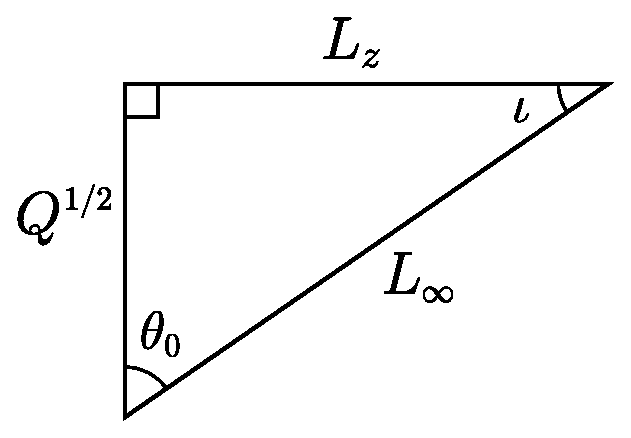
\includegraphics[width=0.2\textwidth]{Triangle.eps}
    \caption{The angular momenta $L_\infty$, $L_z$ and $\sqrt{Q}$ define a right-angled triangle. The acute angles are $\theta_0$, the extremal value of the polar angle, and $\iota$, the orbital inclination \citep*{Glampedakis2002}.}
   \label{fig:L_triangle}
\end{center}
\end{figure}
Let us now introduce a second angular variable \citep{Drasco2004}
\begin{equation}
\zeta = \zeta_0\cos^2\chi.
\end{equation}
Over one $2\pi$ period of $\chi$, $\theta$ oscillates from its minimum value to its maximum and back. The geodesic equation for $\chi$ is
\begin{equation}
\rho^2\diff{\chi}{\tau} = \sqrt{Q + L_z^2},
\end{equation}
and may be integrated simply.

\section{Waveform Construction}\label{sec:Kludge}

For given angular momenta $L_z$ and $Q$, and initial starting position, we can calculate the geodesic trajectory. The orbiting body is assumed to follow this track exactly; we ignore evolution due to the radiation of energy and angular momentum, which should be negligible for EMRBs. From this trajectory we calculate the waveform using a semirelativistic approximation \citep{Ruffini1981}: we assume that the particle moves along a geodesic in the Kerr geometry, but radiates as if it were in flat spacetime. This quick-and-dirty technique is known as a numerical kludge (NK), and has been shown to approximate well results computed by more accurate methods \citep{Babak2007}. It is often compared to a bead travelling along a wire. The shape of the wire is set by the Kerr geodesic, but the bead moves along in flat space.

\subsection{Kludge approximation}

Numerical kludge approximations aim to encapsulate the main characteristics of a waveform by using the exact particle trajectory (ignoring inaccuracies from radiative effects and from the particle's self-force), whilst saving on computational time by using approximate waveform generation techniques.

To start, we build an equivalent flat-space trajectory from the Kerr geodesic. This is done by identifying the Boyer-Lindquist coordinates with a set of flat-space coordinates. We consider two choices here:
\begin{enumerate}
\item Identify the Boyer-Lindquist coordinates with flat-space spherical polars $\{r\sub{BL},$ $\theta\sub{BL},$ $\phi\sub{BL}\} \rightarrow \{r\sub{sph}, \theta\sub{sph}, \phi\sub{sph}\}$, then define flat-space Cartesian coordinates \citep{Gair2005, Babak2007}
\begin{equation}
\boldsymbol{x} = \begin{pmatrix}
r\sub{sph} \sin\theta\sub{sph}\cos\phi\sub{sph} \\
r\sub{sph} \sin\theta\sub{sph}\sin\phi\sub{sph} \\
r\sub{sph} \cos\theta\sub{sph}
\end{pmatrix}.
\end{equation}
\item Identify the Boyer-Lindquist coordinates with flat-space oblate-spheroidal coordinates $\{r\sub{BL}, \theta\sub{BL}, \phi\sub{BL}\} \rightarrow \{r\sub{ob}, \theta\sub{ob}, \phi\sub{ob}\}$ so that the flat-space Cartesian coordinates are
\begin{equation}
\boldsymbol{x} = \begin{pmatrix}
\sqrt{{r\sub{ob}}^2 + a^2} \sin\theta\sub{ob}\cos\phi\sub{ob} \\
\sqrt{{r\sub{ob}}^2 + a^2} \sin\theta\sub{ob}\sin\phi\sub{ob} \\
r\sub{ob} \cos\theta\sub{ob}
\end{pmatrix}.
\end{equation}
These are appealing because in the limit that $G \rightarrow 0$, where the gravitating mass goes to zero, the Kerr metric in Boyer-Lindquist coordinates reduces to the Minkowski metric in oblate-spheroidal coordinates.
\end{enumerate}
In the limit of $a \rightarrow 0$, the two coincide, as they do in the limit of large $r$.

It must be stressed that there is no well motivated argument that either coordinate system must yield an accurate GW; their use is justified {\it post facto} by comparison with results obtained from more accurate, and computationally intensive, methods \citep{Gair2005, Babak2007}. The ambiguity in assigning flat-space coordinates reflects the inconsistency of the semirelativistic approximation: the geodesic trajectory was calculated for the Kerr geometry; by moving to flat spacetime we lose the reason for its existence. However, this inconsistency should not be regarded as a major problem; it is just an artifact of the basic assumption that the shape of the trajectory is important for determining the character of the radiation, but the curvature of the spacetime in the vicinity of the source is not. By binding the particle to the exact geodesic, we ensure that the kludge waveform has spectral components at the correct frequencies, but by assuming flat spacetime for generation of GWs they shall not have the correct amplitudes.

\subsection{Quadrupole-octupole formula}

Now we have a flat-space particle trajectory $x\sub{P}^\mu(\tau)$, we may apply a flat-space wave generation formula. We use the quadrupole-octupole formula to calculate the gravitational strain \citep{Bekenstein1973, Press1977, Yunes2008}
\begin{equation}
h^{jk}(t, \boldsymbol{x}) = -\frac{2G}{c^6r}\left(\ddot{I}^{jk} - 2n_i\ddot{S}^{ijk} + n_i\dddot{M}^{ijk}\right)_{t'\, =\, t - r/c},
\label{eq:octupole}
\end{equation}
where an over-dot represents differentiation with respect to time $t$ (and not $\tau$), $t'$ is the retarded time, $r = \left|\boldsymbol{x} - \boldsymbol{x}\sub{P}\right|$ is the radial distance, $\boldsymbol{n}$ is the radial unit vector, and the mass quadrupole ${I}^{jk}$, current quadrupole ${S}^{ijk}$ and mass octupole ${M}^{ijk}$ are defined by
\begin{align}
{I}^{jk}\left(t'\right) = {} & \intd{}{}{{x'}^j{x'}^kT^{00}\left(t', \boldsymbol{x'}\right) }{^3x'};\\
{S}^{ijk}\left(t'\right) = {} & \intd{}{}{{x'}^j{x'}^kT^{0i}\left(t', \boldsymbol{x'}\right)}{^3x'};\\
{M}^{ijk}\left(t'\right)  = {} & \recip{c}\intd{}{}{{x'}^i{x'}^j{x'}^kT^{00}\left(t', \boldsymbol{x'}\right)}{^3x'}.
\end{align}
This is correct for a slowly moving source. It is the familiar quadrupole formula (\citealt*{Misner1973}, section 36.10; \citealt{Hobson2006}, section 17.9), derived from linearized theory, plus the next order terms. For a point mass, the energy-momentum tensor $T^{\mu\nu}$ contains a $\delta$-function which allows easy evaluation of the integrals of the various moments to give
\begin{align}
{I}^{jk} = {} & c^2\mu x\sub{P}^jx\sub{P}^k;\\
{S}^{ijk} = {} & c\mu v\sub{P}^ix\sub{P}^jx\sub{P}^k;\\
{M}^{ijk} = {} & c\mu x\sub{P}^ix\sub{P}^jx\sub{P}^k.
\end{align}

Since we are only interested in GWs, we use the transverse-traceless (TT) gauge. The waveform is given in the TT gauge by (\citealt{Misner1973}, box 35.1)
\begin{equation}
h\super{TT}_{jk} = P^l_jh_{lm}P^m_k - \recip{2}P_{jk}P^{lm}h_{lm},
\end{equation}
where the (spatial) projection operator $P_{ij}$ is
\begin{equation}
P_{ij} = \delta_{ij} - n_in_j.
\end{equation}

\section{Detection with \textit{LISA}}\label{sec:Detector}

The classic \textit{LISA} design is a three arm, space-borne laser interferometer \citep{Bender1998, Danzmann2003}. The three arms form an equilateral triangle that rotates as the system's centre of mass follows a circular, heliocentric orbit, trailing $20^{\circ}$ behind the Earth. \textit{eLISA} has a similar design, but trails $9^{\circ}$ behind the Earth and only has two arms, which are shorter in length \citep{Jennrich2011}.

To describe the detector configuration, and to transform from the MBH coordinate system to those of the detector, we find it useful to define three coordinate systems: those of the BH at the GC $x_\bullet^i$; ecliptic coordinates centred at the solar system (SS) barycentre $x_\odot^i$, and coordinates that co-rotate with the detector $x\sub{d}^i$. The MBH's coordinate system and the SS coordinate system are depicted in \figref{BH_SS}.
\begin{figure}
\begin{center}
 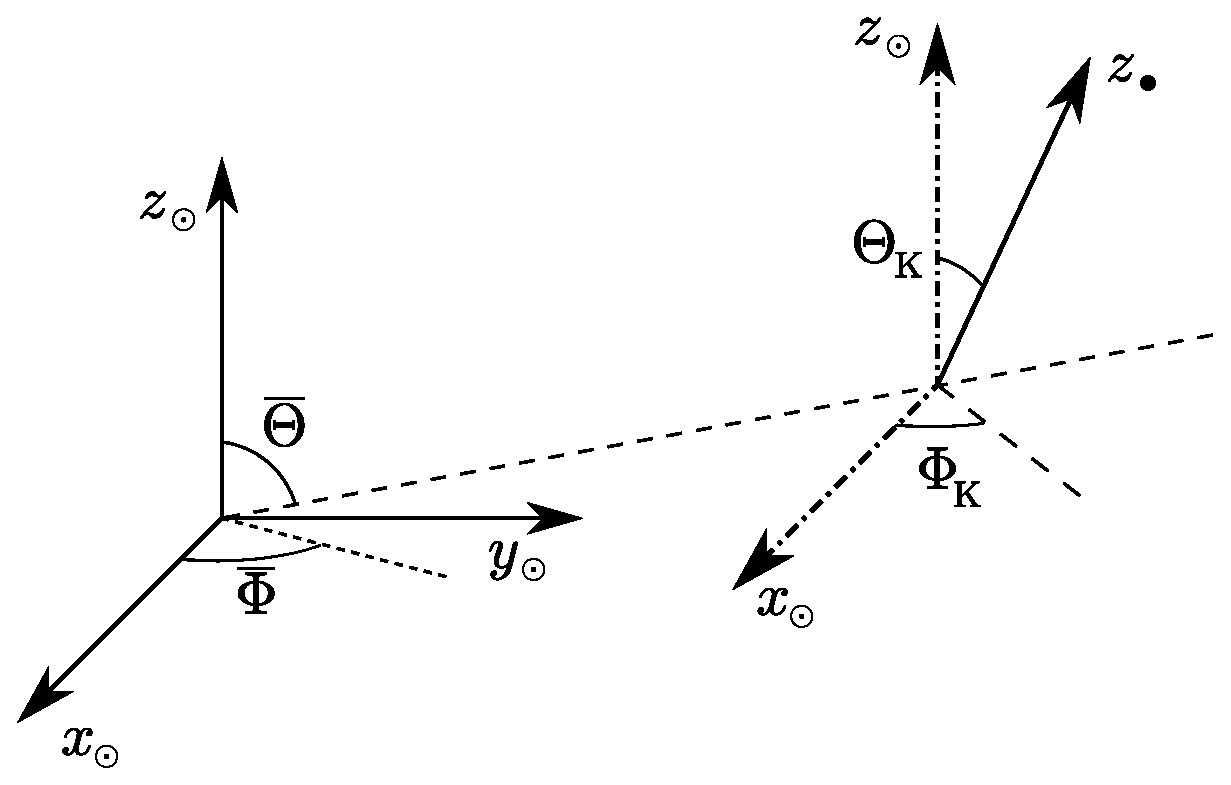
\includegraphics[width=0.35\textwidth]{BH_SS_angles.eps}
    \caption{The relationship between the MBH's coordinate system $x_\bullet^i$ and the SS coordinate system $x_\odot^i$. The MBH's spin axis is aligned with the $z_\bullet$-axis. The orientation of the MBH's $x$- and $y$-axes is arbitrary. We choose $x_\bullet$ to be orthogonal to the direction to the SS.}
   \label{fig:BH_SS}
\end{center}
\end{figure}
The mission geometry for \textit{LISA}/\textit{eLISA} is shown in \figref{SS_LISA}.
\begin{figure}
\begin{center}
 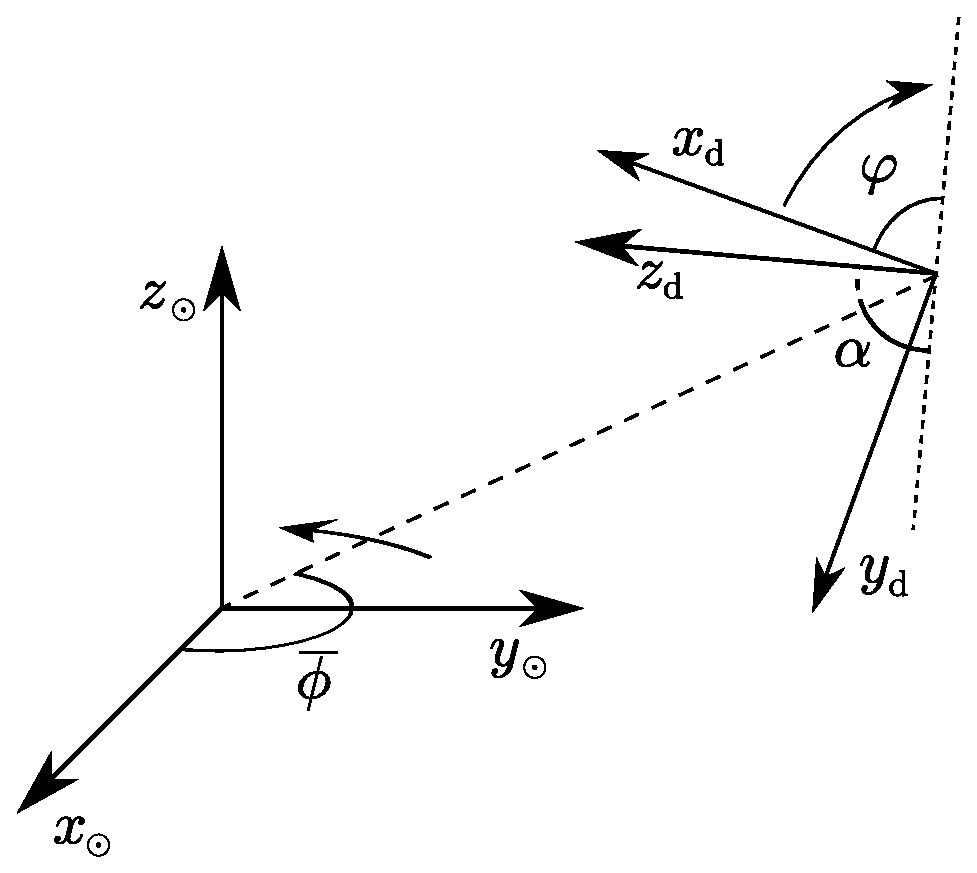
\includegraphics[width=0.27\textwidth]{SS_LISA.eps}
    \caption{The relationship between the detector coordinates $x\sub{d}^i$ and the ecliptic coordinates of the SS $x_\odot^i$ \citep{Bender1998, Jennrich2011}.}
   \label{fig:SS_LISA}
\end{center}
\end{figure}
We define the detector coordinates such that the detector-arms lie in the $x\sub{d}$-$y\sub{d}$ plane as shown in \figref{LISA_arms}.
\begin{figure}
\begin{center}
 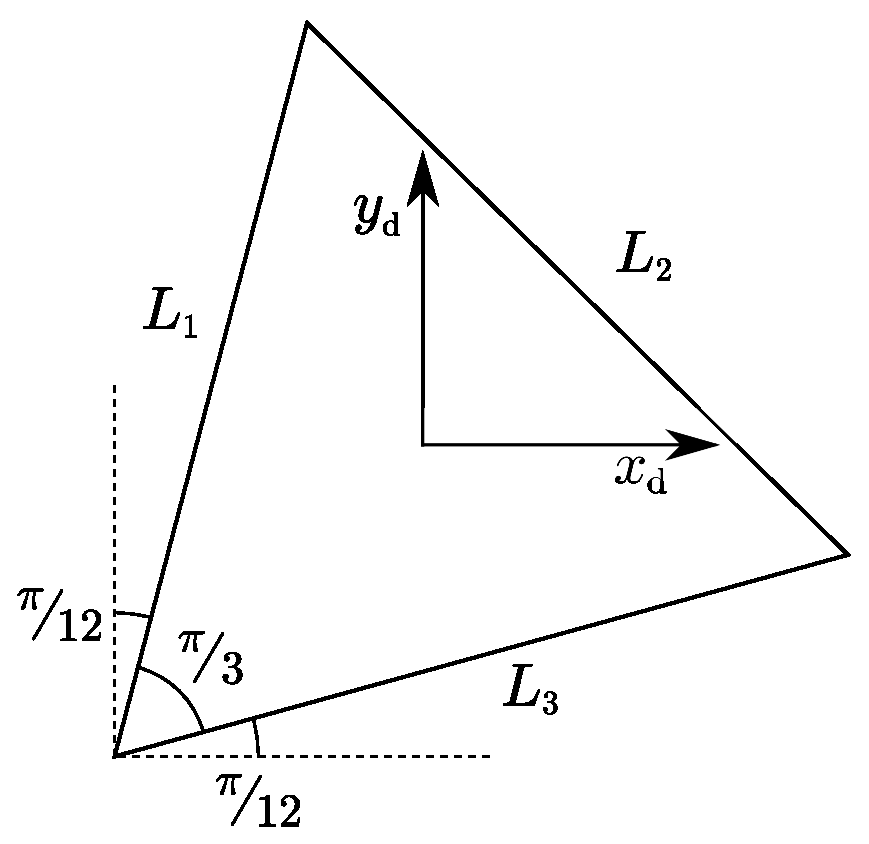
\includegraphics[width=0.25\textwidth]{LISA_arms.eps}
    \caption{The alignment of the three detector arms, with lengths $L_1$, $L_2$ and $L_3$, within the $x\sub{d}$-$y\sub{d}$ plane \citep{Cutler1998}. The origin of the detector coordinates coincides with the centre of mass of the constellation of satellites.}
   \label{fig:LISA_arms}
\end{center}
\end{figure}
The coordinate systems are related by a series of angles: $\Theta\sub{K}$ and $\Phi\sub{K}$ give the orientation of the MBH's spin axis relative to the SS's coordinates. $\overline{\Theta}$ and $\overline{\Phi}$ give the position of the GC in ecliptic coordinates. $\overline{\phi}$ gives the detector's orbital phase and $\varphi$ gives the rotational phase of the detector arms. Both of these vary linearly with time
\begin{equation}
\overline{\phi}(t) = \omega_\oplus t + \overline{\phi}_0; \quad \varphi(t) = -\omega_\oplus t + \varphi_0;
\end{equation}
where $\omega_\oplus$ corresponds to one rotation per year. Finally, $\alpha = 60^{\circ}$ is the inclination of the detector plane. We have computed the waveforms in the MBH's coordinates, however it is simplest to describe the measured signal using the detector's coordinates.

The strains measured in the three arms can be combined such that \textit{LISA} behaves as a pair of $90^{\circ}$ interferometers at $45^{\circ}$ to each other, with signals scaled by ${\sqrt{3}}/{2}$ \citep{Cutler1998}. We denote the two detectors as I and II. If we label the change in the three arms' lengths caused by GWs $\delta L_1$, $\delta L_2$ and $\delta L_3$, and use $L$ for the unperturbed length, then detector I measures strain
\begin{equation}
h\sub{I}(t) = \frac{\delta L_1 - \delta L_2}{L} = \frac{\sqrt{3}}{2}\left(\recip{2} h\sub{d}^{xx} - \recip{2}h\sub{d}^{yy}\right),
\end{equation}
and detector II measures
\begin{equation}
h\sub{II}(t) = \frac{\delta L_1 + \delta L_2 - 2 \delta L_3}{\sqrt{3}L} = \frac{\sqrt{3}}{2}\left(\recip{2} h\sub{d}^{xy} + \recip{2} h\sub{d}^{yx}\right).
\end{equation}
We use vector notation $\boldsymbol{h}(t) = \left(h\sub{I}(t), h\sub{II}(t)\right) = \left\{h_A(t)\right\}$ to represent signals from both detectors.

The final consideration for calculating the signal measured by \textit{LISA} is the time of arrival of the signal: \textit{LISA}'s orbital position changes with time. Fortunately over the timescales of interest for EMRBs, these changes are small. We assume that the position of the SS barycentre relative to the GC is constant: it is defined by the distance $R_0$ and the angles $\overline{\Theta}$ and $\overline{\Phi}$. The time of arrival at the SS barycentre $t_\odot$ is then the retarded time; the time of detection $t\sub{d}$ is
\begin{equation}
t\sub{d} \simeq t_\odot - t\sub{AU}\cos\left[\overline{\phi}(t_\odot) - \overline{\Phi}\right]\sin\overline{\Theta},
\end{equation}
where $t\sub{AU}$ is the light travel-time for the detector's orbital radius. The time $t\sub{d}$ is required for $\phi(t)$ and $\varphi(t)$.

\section{Signal analysis}\label{sec:Signal}

\subsection{Frequency domain formalism}

Having constructed the GW $\boldsymbol{h}(t)$ that shall be incident upon the detector, we may now consider how to analyse the waveform and extract the information it contains. We begin with a brief overview of the basic components of signal analysis used for GWs, with application to \textit{LISA} in particular. This fixes notation. A more complete discussion can be found in \citet{Finn1992}, and \citet{Cutler1994}. Adaption for \textit{eLISA} requires a substitution of the noise distribution, and the removal of the sum over data channels, since it will only have one.

The measured strain $\boldsymbol{s}(t)$ is the combination of the signal and the detector noise
\begin{equation}
\boldsymbol{s}(t) = \boldsymbol{h}(t) + \boldsymbol{n}(t);
\end{equation}
we assume that the noise $n_A(t)$ is stationary and Gaussian. It is more convenient to work with the Fourier transform
\begin{equation}
\tilde{g}(f) = \mathscr{F}\{g(t)\} = \intd{-\infty}{\infty}{g(t)e^{2\pi i ft}}{t}.
\end{equation}
For a Gaussian noise signal $n_A(t)$, each Fourier component $\tilde{n}_A(f)$ has a Gaussian probability distribution; the assumption of stationarity means that different Fourier components are uncorrelated, thus \citep{Cutler1994}
\begin{equation}
\left\langle\tilde{n}_A(f)\tilde{n}_B^*(f')\right\rangle_n = \recip{2}\delta(f - f')S_{AB}(f),
\end{equation}
where $\left\langle\ldots\right\rangle_n$ denotes the expectation value over the noise distribution, and $S_{AB}(f)$ is the (single-sided) noise spectral density. For simplicity, we may assume that the noise in the two detectors is uncorrelated, but share the same characterisation so that \citep{Cutler1998}
\begin{equation}
S_{AB}(f) = S_n(f)\delta_{AB}.
\end{equation}

The properties of the noise allow us to define a natural inner product and associated distance on the space of signals \citep{Cutler1994}
\begin{equation}
\innerprod{\boldsymbol{g}}{\boldsymbol{k}} = 2\intd{0}{\infty}{\frac{\tilde{g}_A^\ast(f)\tilde{k}_A(f) + \tilde{g}_A(f)\tilde{k}_A^\ast(f)}{S_n(f)}}{f}.
\label{eq:inner}
\end{equation}
Using this definition, the signal-to-noise ratio is approximately
\begin{equation}
\rho[\boldsymbol{h}] = \innerprod{\boldsymbol{h}}{\boldsymbol{h}}^{1/2}.
\label{eq:SNR}
\end{equation}
The probability of a particular realization of noise $\boldsymbol{n}(t) = \boldsymbol{n}_0(t)$ is
\begin{equation}
p(\boldsymbol{n}(t) = \boldsymbol{n}_0(t)) \propto \exp\left[-\recip{2}\innerprod{\boldsymbol{n}_0}{\boldsymbol{n}_0}\right].
\end{equation}
If the incident waveform is $\boldsymbol{h}(t)$, the probability of measuring signal $\boldsymbol{s}(t)$ is
\begin{equation}
p(\boldsymbol{s}(t)|\boldsymbol{h}(t)) \propto \exp\left[-\recip{2}\innerprod{\boldsymbol{s}-\boldsymbol{h}}{\boldsymbol{s}-\boldsymbol{h}}\right].
\label{eq:sig_prob}
\end{equation}

\subsection{Noise curve}\label{sec:Noise}

\textit{LISA}'s noise has two sources: instrumental noise and confusion noise, primarily from white dwarf binaries. The latter may be divided into contributions from galactic and extragalactic binaries. In this work we use the noise model of \citet{Barack2004}. The shape of the noise curve can be seen in \figref{Noise}. The instrumental noise dominates at both high and low frequencies. The confusion noise is important at intermediate frequencies, and is responsible for the cusp around $10^{-3}\units{Hz}$. \textit{eLISA} shares the same sources of noise, but is less affected by confusion. Its sensitivity regime is shifted to higher frequencies because of a shorter arm length.
\begin{figure}
\begin{center}
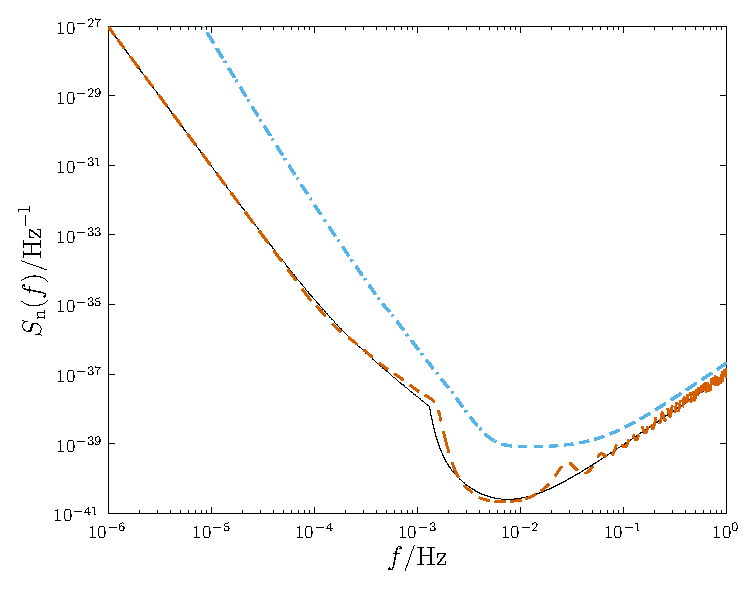
\includegraphics[width=0.45\textwidth]{Fig_Noise}
\caption{The detector noise curves. The solid line indicates the analytic approximation of \citet{Barack2004} used in this work. For comparison, the dashed line is from the online \textit{LISA} sensitivity curve generator (\url{http://www.srl.caltech.edu/~shane/sensitivity/}; \citealt*{Larson2000, Larson2002}). For bursts from the Galactic Centre we are most interested in the low-frequency region where the two curves are the same. The dot-dashed line shows the \textit{eLISA} noise curve.}
\label{fig:Noise}
\end{center}
\end{figure}

\subsection{Window functions}

There is one remaining complication regarding signal analysis: since we are Fourier transforming a finite signal we encounter spectral leakage; a contribution from large amplitude spectral components leaks into surrounding components (sidelobes), obscuring and distorting the spectrum at these frequencies \citep{Harris1978}. This is an inherent problem with finite signals; it shall be as much of a problem when analysing signals from an actual mission as it is computing waveforms here. To mitigate, but unfortunately not eliminate, these effects, the time-domain signal can be multiplied by a window function. These are discussed in detail in \apref{window}. We have adopted the Nuttall four-term window with continuous first derivative \citep{Nuttall1981} for the results presented here.

\section{Waveforms and detectability}\label{sec:Waveforms}

\subsection{Model parameters}

The shape of the waveform depends on a number of parameters: those defining the MBH; those defining the companion object on its orbit, and those defining the \textit{LISA} detector. Let us define $\boldsymbol{\lambda} = \left\{\lambda^1, \lambda^2, \ldots, \lambda^Z\right\}$ as the set of $Z$ parameters which specify the GW. For our model, the input parameters are:
\begin{enumerate}
\item[(1)] The MBH's mass $M_\bullet$. This is currently well constrained by the observation of stellar orbits about Sgr A* \citep{Ghez2008, Gillessen2009}, with the best estimate being $M_\bullet = (4.31 \pm 0.36) \times 10^6 M_\odot$. This depends upon the galactic centre distance $R_0$ as $M_\bullet = (3.95 \pm 0.06|\sub{stat} \pm 0.18|_{R_0, \, \mathrm{stat}} \pm  0.31|_{R_0, \, \mathrm{sys}}) \times 10^6 M_\odot (R_0 / 8\units{kpc})^{2.19}$, where the errors are statistical, independent of $R_0$; statistical from the determination of $R_0$, and systematic from $R_0$ respectively.
\item[(2)] The spin parameter $a_\ast$. Naively this could be anywhere in the range $|a_\ast| < 1$; however it is possible to place an upper bound by contemplating spin-up mechanisms. Considering the torque from radiation emitted by an accretion disc, and swallowed by the BH, it can be shown that $|a_\ast| \lesssim 0.998$ \citep{Thorne1974}. Magnetohydrodynamical simulations of accretion discs produce a smaller maximum value of $|a_\ast| \sim 0.95$ \citep{Gammie2004}. The actual spin value could be much lower than this upper bound depending upon the MBH's evolution (as discussed in \secref{Intro}).
\item[(3,4)] The orientation angles for the black hole spin $\Theta\sub{K}$ and $\Phi\sub{K}$.
\item[(5)] The ratio of the SS-GC distance $R_0$ and the CO mass $\mu$, which we denote as $\zeta = R_0/\mu$. This scales the amplitude of the waveform. Bursts, unlike inspirals, do not undergo orbital evolution, hence we cannot break the degeneracy in $R_0$ and $\mu$, and they cannot be inferred separately. The distance, like $M_\bullet$, is constrained by stellar orbits, the best estimate being \citep{Gillessen2009} $R_0 = 8.33 \pm 0.35\units{kpc}$. The mass of the orbiting particle depends upon the type of object: whether it is an MS star, WD, NS or BH. Since we shall not know the $\mu$ precisely, we shall not be able to infer anything more about the distance to the GC.
\item[(6, 7)] The angular momentum of the CO. This can be described using either $\{L_z, Q\}$ or $\{L_\infty, \iota\}$. We employ the latter, as the total angular momentum and inclination are less tightly correlated. Assuming spherical symmetry, we expect $\cos \iota$ to be uniformly distributed.
\item[(8--10)] A set of coordinates to specify the trajectory. These could be positions at an arbitrary time. We use the angular phases at periapse, $\phi\sub{p}$ and $\chi\sub{p}$ (which determines $\theta\sub{p}$), as well as the time of periapse $t\sub{p}$.
\item[(11, 12)] The coordinates of the MBH from the SS barycentre $\overline{\Theta}$ and $\overline{\Phi}$. These may be taken as the coordinates of Sgr A*, as the radio source is expected to be within ten Schwarzschild radii of the MBH \citep{Reid2003,Doeleman2008}. At the epoch J2000.0 $\overline{\Theta} = {95.607669}^{\circ}$, $\overline{\Phi} = {266.851760}^{\circ}$ \citep{Reid1999, Yusef-Zadeh1999}. They change with time due to the rotation of the SS about the GC; the proper motion is about $6\units{mas\,yr^{-1}}$, mostly in the plane of the galaxy \citep{Reid1999, Backer1999, Reid2003}. The position is already determined to high accuracy: an EMRB can only give weak constraints on source position.\footnote{For comparison, an EMRI, which should be more informative, can only give sky localisation to $\sim 10^{-3}~\mathrm{steradians}$ \citep{Barack2004, Huerta2009}.} Therefore we take it as known and shall not try to infer it.
\item[(13, 14)] The orbital position of the \textit{LISA} satellites given by $\overline{\phi}$ and $\varphi$. We assume that the initial positions are chosen such that $\overline{\phi} = 0$ when $\varphi = 0$ \citep{Cutler1998}; this choice does not qualitatively influence our results. The orbital position should be known, so this need not be inferred.\\
\end{enumerate}
We therefore have a $14$ dimensional parameter space, of which we are interested in inferring $d = 10$ parameters.

\subsection{Waveforms}

\Figref{Examples} shows example waveforms to demonstrate some of the possible variations in the signal. All these assume the standard mass and position for the MBH as well as a $\mu = 10 M_\odot$ orbiting CO; other (randomly chosen) orbital parameters are specified in the captions. Radii are given in terms of the gravitational radius $r\sub{g} = GM_\bullet / c^2$.
\begin{figure}
  \begin{center}
   \subfigure[{Waveform for $a_\ast \simeq 0.12$, $r\sub{p} \simeq 15.6 r\sub{g}$ and $\iota \simeq 2.1$. The SNR for the spherical polar kludge waveform (plotted) is $\rho[\boldsymbol{h}\sub{sph}] \simeq 451$, for the oblate-spheroidal kludge it is $\rho[\boldsymbol{h}\sub{ob}] \simeq 451$ (agreement to $0.01\%$).}]{\label{fig:Orbit_233} \includegraphics[width=0.45\textwidth]{Fig_new_sph_h_233}} \\
   \subfigure[{Waveform for $a_\ast \simeq 0.48$, $r\sub{p} \simeq 8.8 r\sub{g}$ and $\iota \simeq 2.0$. The SNR for the spherical polar kludge waveform (plotted) is $\rho[\boldsymbol{h}\sub{sph}] \simeq 2300$, for the oblate-spheroidal kludge it is $\rho[\boldsymbol{h}\sub{ob}] \simeq 2310$.}]{\label{fig:Orbit_254} 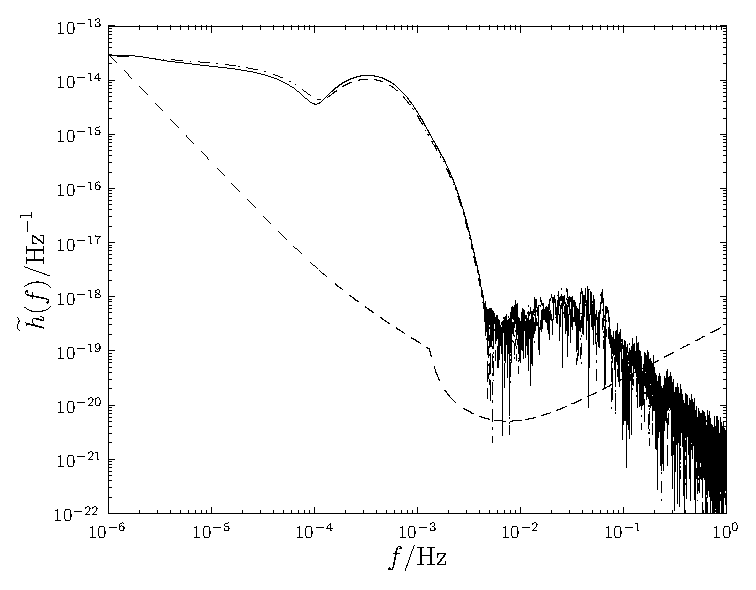
\includegraphics[width=0.45\textwidth]{Fig_new_sph_h_254}} \\
   \subfigure[{Waveform for $a_\ast \simeq 0.74$, $r\sub{p} \simeq 3.2 r\sub{g}$ and $\iota \simeq 1.2$. The SNR for the spherical polar kludge waveform (plotted) is $\rho[\boldsymbol{h}\sub{sph}] \simeq 70600$, for the oblate-spheroidal kludge it is $\rho[\boldsymbol{h}\sub{ob}] \simeq 74900$.}]{\label{fig:Orbit_135} \includegraphics[width=0.45\textwidth]{Fig_new_sph_h_135}}  
\label{fig:Examples}
\caption{Example burst waveforms from the galactic centre. The strain $\widetilde{h}\sub{I}(f)$ is indicated by the solid line, $\widetilde{h}\sub{II}(f)$ by the dot-dashed line, and the noise curve by the dashed line. The kludge has been formulated using spherical polar coordinates.}
  \end{center}
\end{figure}

The plotted waveforms use the spherical polar coordinate system for the NK. Using oblate-spheroidal coordinates makes a small difference: on the scale shown here the only discernible difference would be in \figref{Orbit_135}; the maximum difference in the waveform (outside the high-frequency tail) is $\sim 10\%$. In the other cases the difference is entirely negligible (except in the high-frequency tail, which is not of physical significance). This behaviour is typical, for the closest orbits, with the most extreme spin parameters, the maximum difference in the waveforms may be $\sim30\%$. The difference is largely confined to the higher frequency components, which are most sensitive to the parts of the trajectory closer to the MBH: the change in flat-space radius for the same Boyer-Lindquist radial coordinate causes a slight shift in the shape of the spectrum. Enforcing the same flat-space periapse radius gives worse agreement across the spectrum.

To examine the effect of the coordinate choice, we compare SNRs calculated using the alternative schemes for a selection of orbits. The MBH parameters were fixed as for the GC, the orbital parameters were chosen such that periapse distance was drawn from a logarithmic distribution (down to the innermost stable orbit), and other parameters were drawn from appropriate uniform distributions. The ratio of the two SNRs is shown in \figref{Oblate_sphere}.
\begin{figure}
\begin{center}
 \includegraphics[width=0.45\textwidth]{Fig_SNR_ratio}
 \label{fig:Oblate_sphere}
 \caption{Ratio of SNR for a waveform calculated using spherical polar coordinates to that for a waveform using oblate-spheroidal coordinates.}
   \end{center}
\end{figure}
The difference from the coordinate systems is only apparent for orbits with very small periapses. There is agreement to $10\%$ down to $r\sub{p} \simeq 4 r\sub{g}$; the maximal difference may be expected to be $\sim 20\%$, this is for periapses that are only obtainable for high spin values.

Since the deviation in the two waveforms is only apparent for small periapses, when the kludge approximation is least applicable, we conclude that the choice of coordinates is unimportant. The potential error of order $10\%$ is no greater than that inherent in the NK approximation (see \secref{Energy}). Without an accurate waveform template to compare against, we do not know if there is a preferable choice of coordinates. We adopt spherical coordinates for easier comparison with existing work.

\subsection{Signal-to-noise ratios}

The detectability of a burst depends upon its SNR. To characterise the variation of $\rho$ we considered a range of orbits. In each case the MBH was assumed to have a mass of $M_\bullet = 4.31 \times 10^6 M_\odot$, to be at the J2000.0 coordinates and a distance of $R_0 = 8.33~\mathrm{kpc}$.

These bursts were calculated for a $1 M_\odot$ CO. From \eqnref{octupole}, the amplitude of the waveform is proportional to the CO mass $\mu$ and so $\rho$ is also proportional to $\mu$; a $10 M_\odot$ object would be ten times louder on the same orbit. To make results mass independent, we shall work in terms of a mass-normalised SNR
\begin{equation}
\hat{\rho}[\boldsymbol{h}] = \left(\frac{\mu}{M_\odot}\right)^{-1}\rho[\boldsymbol{h}].
\end{equation}

The spin of the MBH and the orbital inclination were randomly chosen, and the periapse distance was set so that the distribution would be uniform in log-space (down to the point of the inner-most stable orbit). For each set of these extrinsic parameters, the periapse position, orientation of the MBH, and orbital position of the detector were varied: five random combinations of these intrinsic parameters (each being drawn from a separate uniform distribution) were used for each point.

We take the mean of $\ln \rho$ for each set of randomised intrinsic parameters (starting position, MBH orientation and detector orientation).\footnote{The logarithm is a better quantity to work with since the SNR is a positive-definite quantity that may be distributed over a range of magnitudes \citep[sections 22.1, 23.3]{MacKay2003}. Using median values yields results that are quantitatively similar.}

There exists a correlation between the periapse radius and SNR, as shown in \figref{SNR}.
\begin{figure}
  \begin{center}
  \includegraphics[width=0.45\textwidth]{Fig_SNR}
    \caption{Mass-normalised SNR as a function of periapse radius. The plotted points are the values obtained by averaging over each set of intrinsic parameters. The best fit line is $\log(\hat{\rho}) = -2.69\log(r\sub{p}/r\sub{g}) + 4.88$. This is fitted to orbits with $r\sub{p} >  13.0 r\sub{g}$ and has a reduced chi-squared value of $\chi^2/\nu = 1.73$.}
    \label{fig:SNR}
  \end{center}
\end{figure}
Closer orbits produce louder bursts. To reflect this relationship, we have fitted a simple fiducial power law, as indicated by the straight line.\footnote{Using oblate-spheroidal coordinates instead of spherical polars gives a fit consistent to within $0.1\%$ as we have excluded the closest orbits.} This was done by maximising the likelihood, assuming that $\ln \rho$ has a Gaussian distribution with standard deviation derived from the scatter because of variation in the intrinsic parameters. The power law appears to be a good fit only for orbits with larger periapses. The shape of the curve is predominately determined by the shape of the noise curve. The change in the trend reflects the change as we go from approximately power law behaviour into the bucket of the curve. Hence, we fit a power law to orbits with a characteristic frequency of $f_\ast = \sqrt{GM_\bullet/r\sub{p}} < 1 \times 10^{-3}\units{Hz}$, so as to avoid spilling over into the bucket. Changing the cut-off within a plausible region alters the fit coefficients by around $0.1$.\footnote{The power law exponent $-2.7$ is inconsistent with $-13/4$ as predicted by the approximate model of \citet{Hopman2007}. This is the result of their approximate waveform model.}

The SNR shows no clear correlation with the other parameters (excluding the mass $\mu$). However, the SNR is sensitive to the intrinsic parameters, in particular the initial position (as this determines the subsequent trajectory), and may vary by an order of magnitude.

Setting a threshold of $\rho = 10$, a $1 M_\odot$ ($10 M_\odot$) object would be expected to be detectable if the periapse distance is less than $27 r\sub{g}$ ($65 r\sub{g}$). \citet{Hopman2007}, assuming a threshold of $\rho = 5$, used an approximate form for the SNR based upon the quadrupole component of a circular orbit; their model, with updated parameters for the MBH, predicts bursts would be detectable out to $66 r\sub{g}$ ($135 r\sub{g}$). We see that this is overly optimistic.

\section{Energy spectra}\label{sec:Energy}

To check that the NK waveforms are sensible, we may compare the energy spectra calculated from these with those obtained from the classic treatment of \citet{Peters1963}, and \citet{Peters1964}. This calculates GW emission for Keplerian orbits in flat spacetime, assuming only quadrupole radiation. The spectrum produced should be similar to that obtained from the NK in weak fields, that is for orbits with a large periapsis; however, we do not expect an exact match because of the differing input physics and varying approximations.

In addition to using the energy spectrum, we can also use the total energy flux to check the NK waveforms. The total flux contains less information than the spectrum; however, results have been calculated for parabolic orbits in Schwarzschild spacetime using time-domain black hole perturbation theory \citep{Martel2004}. These should be more accurate than results calculated using the Peters and Mathews formalism.

We do not intend to use the kludge waveforms to calculate an accurate energy flux: this would be inconsistent as we assume that the orbits do not evolve with time. We only calculate the energy flux as a sanity check, to confirm that the kludge approximation is consistent with other approaches.

\subsection{Kludge spectrum}

A gravitational wave in the TT gauge has an effective energy-momentum tensor (\citealt{Misner1973}, section 35.15)
\begin{equation}
T_{\mu\nu} = \frac{c^4}{32\pi G}\left\langle\partial_\mu h_{ij} \partial_\nu h^{ij}\right\rangle,
\end{equation}
where $\langle\ldots\rangle$ indicates averaging over several wavelengths or periods. The flux of energy through a sphere of radius $r = R$ is
\begin{equation}
\diff{E}{t} = \frac{c^3}{32\pi G} R^2 \int{\dd\Omega}\left\langle\diff{h_{ij}}{t}\diff{h^{ij}}{t}\right\rangle,
\end{equation}
with $\int{\dd\Omega}$ representing integration over all solid angles. From \eqnref{octupole} we see that the waves have a $1/{r}$ dependence; if we define
\begin{equation}
h_{ij} = \frac{H_{ij}}{r},
\end{equation}
we see that, using \eqnref{octupole}, the flux is independent of $R$, as required for energy conservation, and
\begin{equation}
\diff{E}{t} = \frac{c^3}{32\pi G} \int{\dd\Omega}\left\langle\diff{H_{ij}}{t}\diff{H^{ij}}{t}\right\rangle.
\end{equation}
If we now integrate to find the total energy emitted we obtain
\begin{equation}
E = \frac{c^3}{32\pi G} \int{\dd\Omega}\int_{-\infty}^{\infty}{\dd t} \, \diff{H_{ij}}{t}\diff{H^{ij}}{t}.
\label{eq:integrate_E}
\end{equation}
Since we are considering all time, the localization of the energy is no longer of importance and it is unnecessary to average over several periods. Switching to Fourier representation $\widetilde{H}_{ij}(f) = \mathscr{F}\left\{H_{ij}(t)\right\}$,
\begin{equation}
E = \frac{\pi c^3}{4 G} \int{\dd\Omega}\int_{0}^{\infty}{\dd f} \, f^2 \widetilde{H}^{ij}(f)\widetilde{H}_{ij}^*(f),
\label{eq:total_E}
\end{equation}
using the fact that the signal is real so $\widetilde{H}_{ij}^*(f) = \widetilde{H}_{ij}(-f)$. From this we identify the energy spectrum as
\begin{align}
\diff{E}{f} = \frac{\pi c^3}{4 G} \intd{}{}{}{\Omega} \, f^2 \widetilde{H}^{ij}(f)\widetilde{H}_{ij}^*(f).
\label{eq:NK_dEdf}
\end{align}

\subsection{Peters and Mathews spectrum}

To calculate the Peters and Mathews energy spectrum for a parabolic orbit, we use the limiting result of \citet{Turner1977}
\begin{align}
\diff{E}{f} = {} & \frac{4\pi^2}{5}\frac{G^3}{c^5}\frac{M_\bullet^2\mu^2}{r\sub{p}^2}\left\{\left[\frac{8f^2}{f\sub{c}^2}B\left(\frac{f}{f\sub{c}}\right) - \frac{2f}{f\sub{c}}A\left(\frac{f}{f\sub{c}}\right)\right]^2 \right. \nonumber \\
 & \left. + \left(\frac{128f^4}{f\sub{c}^4} + \frac{4f^2}{3f\sub{c}^2}\right)\left[A\left(\frac{f}{f\sub{c}}\right)\right]^2\right\},
\label{eq:PM_dEdf}
\end{align}
where $f\sub{c}$ is the orbital frequency of a circular orbit of radius equal to $r\sub{p}$,
\begin{equation}
f\sub{c} = \recip{2\pi}\sqrt{\frac{G(M_\bullet + \mu)}{r\sub{p}^3}},
\end{equation}
and functions $A\left(x\right)$ and $B\left(x\right)$ are defined in terms of Bessel functions. Their precise forms are \citep{Berry2010}
\begin{align}
A\left(x\right) = {} & \recip{\pi}\sqrt{\frac{2}{3}}K_{1/3}\left(\frac{2^{3/2}x}{3}\right); \\
B\left(x\right) = {} & \recip{\sqrt{3}\pi}\left[K_{-2/3}\left(\frac{2^{3/2}x}{3}\right) + K_{4/3}\left(\frac{2^{3/2}x}{3}\right) \right. \nonumber \\
 {} & - \left. \recip{\sqrt{2}x}K_{1/3}\left(\frac{2^{3/2}x}{3}\right)\right],
\end{align}
where $K_\nu(z)$ is a modified Bessel function of the second kind. This result should be accurate to $\sim10\%$ for orbits with periapse radii larger than $\sim20r\sub{g}$ \citep{Berry2010}.

\subsection{Comparison}

Two energy spectra are plotted in \figref{Energy} for orbits with periapses of $r\sub{p} = 15.0 r\sub{g}$, $30.0 r\sub{g}$ and $60.0 r\sub{g}$.
\begin{figure*}
  \begin{center}
   \subfigure[$r\sub{p} = 15.0 r\sub{g}$, log-log plot.]{\includegraphics[width=0.45\textwidth]{Fig_Loglog_E_15}} \quad
   \subfigure[$r\sub{p} = 15.0 r\sub{g}$, log-linear plot.]{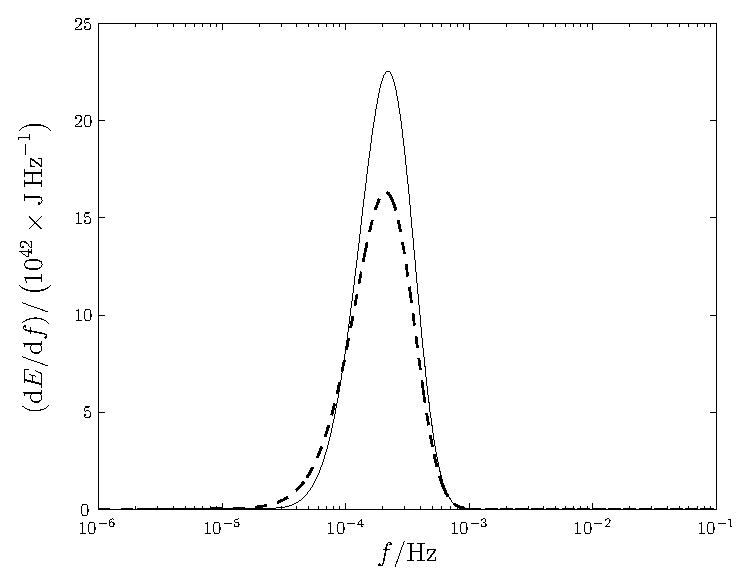
\includegraphics[width=0.45\textwidth]{Fig_Loglin_E_15}} \\
   \subfigure[$r\sub{p} = 30.0 r\sub{g}$, log-log plot.]{\includegraphics[width=0.45\textwidth]{Fig_Loglog_E_30}} \quad
   \subfigure[$r\sub{p} = 30.0 r\sub{g}$, log-linear plot.]{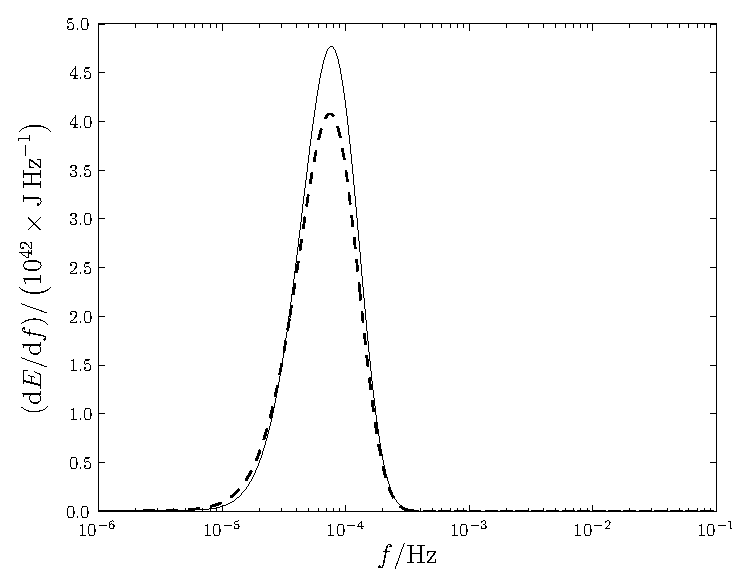
\includegraphics[width=0.45\textwidth]{Fig_Loglin_E_30}} \\
   \subfigure[$r\sub{p} = 60.0 r\sub{g}$, log-log plot.]{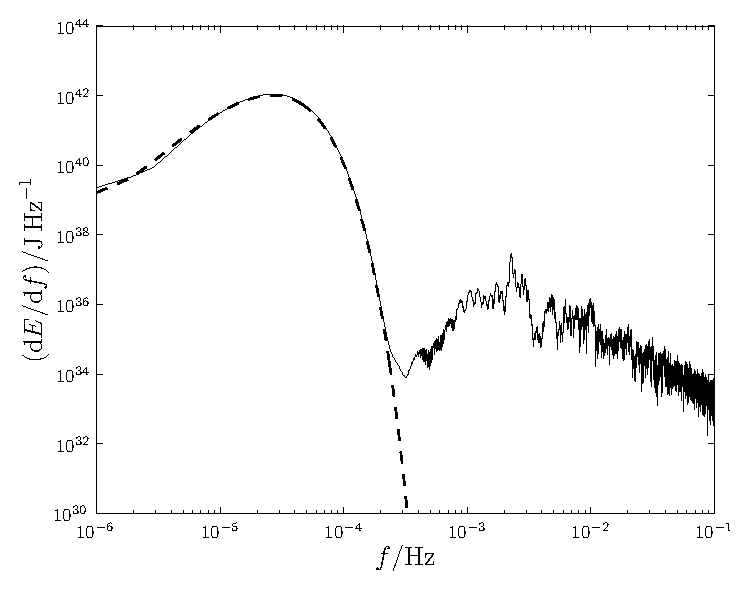
\includegraphics[width=0.45\textwidth]{Fig_Loglog_E_60}} \quad
   \subfigure[$r\sub{p} = 60.0 r\sub{g}$, log-linear plot.]{\includegraphics[width=0.45\textwidth]{Fig_Loglin_E_60}}
    \caption{Energy spectra for a parabolic orbit of a $\mu = 10 M_\odot$ object about a Schwarzschild BH with $M_\bullet = 4.31 \times 10^6 M_\odot$. The spectra calculated from the NK waveform is shown by the solid line and the Peters and Mathews flux is indicated by the dashed line. The NK waveform includes octupole contributions. The high frequency tail is the result of spectral leakage.}
    \label{fig:Energy}
  \end{center}
\end{figure*}
The two spectra appear to be in good agreement, showing the same general shape in the weak-field limit. The NK spectrum is more tightly peaked, but is always within a factor of $2$ at the apex. The peak of the spectrum is shifted to a marginally higher frequency in the NK spectrum primarily because of the addition of the current quadrupole and mass octupole terms.

Comparing the total energy fluxes, ratios of the various energies are plotted in \figref{Energy_ratio}.
\begin{figure*}
  \begin{center}
   \subfigure[Versus periapsis]{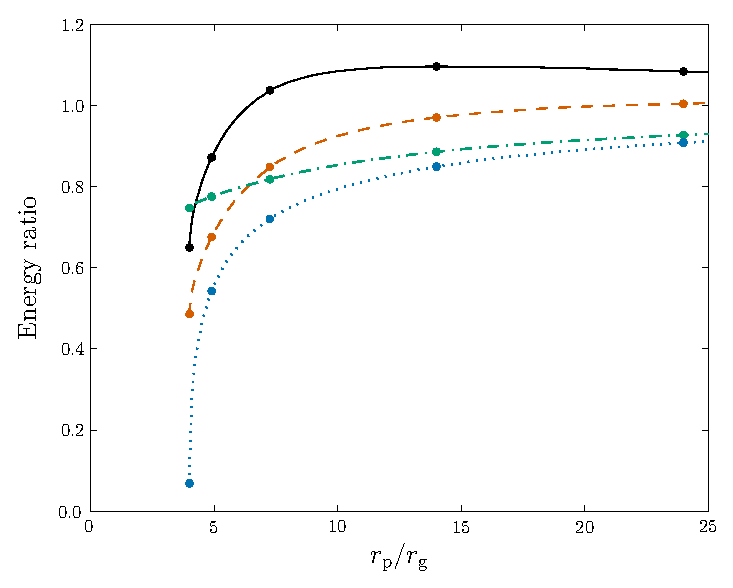
\includegraphics[width=0.45\textwidth]{Fig_Energy_ratio_peri}} \quad
   \subfigure[Versus amount of rotation]{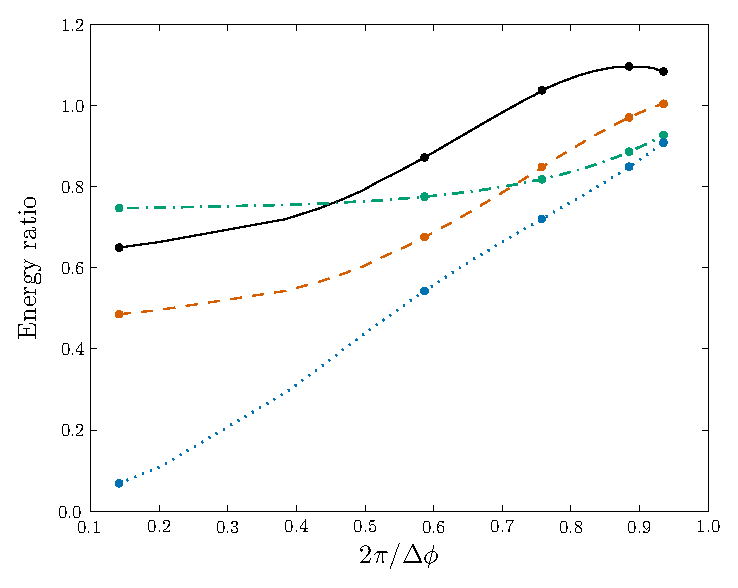
\includegraphics[width=0.45\textwidth]{Fig_Energy_ratio_orbit}}
    \caption{Ratios of energies as a function of periapsis $r\sub{p}$ and $2\pi$ divided by the total angle of rotation in one orbit $\Delta\phi$ ($2\pi/\Delta\phi = 1$ for a Keplerian orbit). The solid line shows the ratio of the numerical kludge and Martel energies $E\sub{NK}/E\sub{M}$; the dashed line shows the ratio of the NK energy calculated using only the mass quadrupole term and the Martel energy $E\sub{NK(Q)}/E\sub{M}$; the dot-dashed line shows the ratio of the quadrupole and quadrupole-octupole NK energies $E\sub{NK(Q)}/E\sub{NK}$, and the dotted line shows the ratio of the Peters and Mathews and quadrupole NK energies $E\sub{PM}/E\sub{NK(Q)}$. The spots show the mapping between the two abscissa scales. Compare with figure 4 of \citet{Gair2005}.}
    \label{fig:Energy_ratio}
  \end{center}
\end{figure*}
We introduce an additional energy here, the quadrupole NK energy $E\sub{NK(Q)}$. This allows easier comparison with the Peters and Mathews energy which includes only quadrupole radiation. It can be calculated in three ways:
\begin{enumerate}
\item Inserting the waveform $\widetilde{h}(f)$ generated including only the mass quadrupole term in \eqnref{octupole} into \eqnref{total_E} and integrating. This is equivalent to the method used to calculate $E\sub{NK}$.
\item Numerically integrating the quadrupole GW luminosity (\citealt{Misner1973}, section 36.7; \citealt{Hobson2006}, section 18.7)
\begin{equation}
E = \frac{G}{5c^9}\intd{}{}{\dddot{\Ibar}_{ij}\dddot{\Ibar}^{ij}}{t},
\label{eq:E_quad}
\end{equation}
where $\Ibar_{ij} = I_{ij} - (1/3)I\delta_{ij}$ is the reduced mass quadrupole tensor. We can obtain this from \eqnref{integrate_E}, by integrating over all angles when the waveform only contains the mass quadrupole component. This has the advantage of avoiding the effects of spectral leakage or the influence of window functions.
\item Using the analytic expressions for the integral \eqnref{E_quad} given in appendix A of \citet{Gair2005}.
\end{enumerate}
All three agree to within computational error. No difference is visible on the scale plotted in \figref{Energy_ratio}. This demonstrates the validity of the code, and shows that the use of a window function does not significantly distort the waveform.

The ratios all tend towards one in the weak field, as required, but differences become more pronounced in the strong field. The NK energy is larger than the Peters and Mathews result $E\sub{PM}$. This behaviour has been seen before for high eccentricity orbits about a non-spinning BH \citep{Gair2005}. It may be explained by considering the total path length for the different orbits: the Peters and Mathews spectrum assumes a Keplerian orbit, the orbit in Kerr geometry rotates more than this. The greater path length leads to increased emission of gravitational waves and a larger energy flux \citep{Berry2010}. Our bead must travel further along its wire. A good proxy for the path length is the angle of rotation $\Delta\phi$; this is $2\pi$ for a Keplerian orbit, in Kerr the angle should be $2\pi$ in the limit of an infinite periapsis, whereas for a periapsis small enough that the orbit shows zoom-whirl behaviour, the total angle may be many times $2\pi$. There is a reasonable correlation between the amount of rotation $2\pi/\Delta\phi$ and the ratio of energies.

Error in the NK energy compared with the time-domain black hole perturbation theory results of Martel comes from two sources: the neglecting of higher order multipole contributions and the ignoring of background curvature. The contribution of the former can be estimated by looking at the difference in the NK energy by including the current quadrupole and mass octupole terms. From \figref{Energy_ratio} we see that these terms give a negligible contribution in the weak field, but the difference is $\sim20\%$ in the strong field. This explains why the Martel energy $E\sub{M}$ is greater in the strong field, as it includes contributions from all multipoles. Neglecting the background curvature increases the NK energy relative to $E\sub{M}$. This partially cancels out the error introduced by not including higher order terms: this accidentally leads to $E\sub{NK(Q)}$ being more accurate than $E\sub{NK}$ for $r\sub{p} \gtrsim 10 r\sub{g}$ \citep{Tanaka1993}.

From the level of agreement we may be confident that the NK waveforms are a reasonable approximation. The difference in energy flux is only greater than $10\%$ for very strong fields $r\sub{p} \simeq 4 r\sub{g}$; since this is dependent on the square of the waveform, typical accuracy in the waveform may be $\sim 5\%$ \citep{Gair2005,Tanaka1993}. This is more significant than the variation in waveforms we generally found using the two alternative coordinate systems for the NK (in this case the two coincide because $a_\ast = 0$).

\section{Discussion}\label{sec:End}

We have outlined an approximate method of generating gravitational waveforms for EMRBs originating at the GC. This assumes that the orbits are parabolic and employs a numerical kludge approximation. The two coordinate schemes for a NK presented here yield almost indistinguishable results. We conclude that either is a valid choice for this purpose. There may be differences when the spin is large and the periapse is small: $\sim 10\%$ for $r\sub{p} \simeq 4 r\sub{g}$, $\sim 20\%$ for $r\sub{p} \simeq 2 r\sub{g}$.

The waveforms created appear to be consistent with results obtained using Peters and Mathews waveforms for large periapses, indicating that they have the correct weak-field form. The NK approach should be superior to that of Peters and Mathews in the strong-field regime as it uses the exact geodesics of the Kerr spacetime. Comparisons with energy fluxes from black hole perturbation theory indicate that typical waveform accuracy may be of order $5\%$, but this is worse for orbits with small periapses, and may be $\sim 20\%$. These errors are greater than the differences resulting from the use of the alternative coordinate systems.

The signal-to-noise ratio of bursts is well correlated with the periapsis. Except for the closest orbits ($r\sub{p} \lesssim 7 r\sub{g}$), the SNR (per unit mass) may be reasonably described as having a power-law dependence of
\begin{equation}
\log\left(\hat{\rho}\right) \simeq -2.7\log\left(\frac{r\sub{p}}{r\sub{g}}\right) + 4.9.
\end{equation}
Signals should be detectable for a $1 M_\odot$ ($10 M_\odot$) object if the periapse is $r\sub{p} < 27 r\sub{g}$ ($r\sub{p} < 65 r\sub{g}$), corresponding to a physical scale of $1.7 \times 10^{11}\units{m}$ ($4.1 \times 10^{11}\units{m}$) or $5.6 \times 10^{-6}\units{pc}$ ($1.3 \times 10^{-5}\units{pc}$).

Using the NK waveforms we conducted an investigation, using Fisher matrix analysis, into how precisely we could infer parameters of the galactic centre's MBH should such an EMRB be observed. However, we found that the linearised-signal approximation (LSA) does not hold for these burst signals over a wide range of SNR. This demonstrates the necessity of checking the LSA before quoting the results of a Fisher matrix analysis~\citep{Vallisneri2008}.

We used MCMC results as a more robust measure of parameter estimation accuracy. Potentially, it is possible to determine very precisely the key parameters defining the MBH's mass and spin, if the orbit gets close enough to the MBH. From our investigation it appears that we can achieve good results from a single EMRB with periapsis of $r\sub{p} \simeq 10 r\sub{g}$ for a $10 M_\odot$ CO. This translates to a distance of $6 \times 10^{10}\units{m}$ or $2 \times 10^{-6}\units{pc}$. Orbits closer than this would be even better, and place stricter constraints. The best orbits yield uncertainties of almost one part in $10^5$ for the MBH mass and spin, far exceeding existing techniques. Conversely, orbits with $r\sub{p} \gtrsim 20 r\sub{g}$ are unlikely to provide any useful information.

Before we can quote results for how accurately we can determine the various parameters, we must consider the probability of each orbit. This will be the subject of a companion paper, building upon the earlier results of \citet{Rubbo2006} and \citet{Hopman2007}, who only considered approximate forms for the SNR, rather than using waveforms. Using a model for the nuclear star cluster of the GC it is possible to define distributions for angular momenta $L_\infty$, for a species of mass $\mu$. With these it is possible to estimate the event rate. This would allow us to estimate how much information, on average, we could hope to obtain from EMRB observations. If it is likely that we would observe multiple EMRBs, it may be possible to combine results to tighten uncertainties.

Some consideration should also be given to methods of fitting a waveform to an observed signal. Given a noisy data stream, how could EMRBs be extracted? The parabolic spectrum has a characteristic profile, suggesting that matched filtering could be possible. Complications could arise in fitting parameters to a waveform: we have seen that there exist complicated degeneracies between parameters. These issues would warrant further investigation should the event rate be high enough.

While we have only considered bursts from our own galaxy in detail, it should be possible to observe bursts from other nearby galaxies if their MBH is of the appropriate mass. This makes M32 as a viable candidate. The SNR shows a similar dependence upon periapsis as for the GC, and may be described by a power-law of
\begin{equation}
\log\left(\hat{\rho}\right) \simeq -2.7\log\left(\frac{r\sub{p}}{r\sub{g}}\right) + 3.1,
\end{equation}
for orbits with $r\sub{p} \gtrsim 10 r\sub{g}$. For a $1 M_\odot$ ($10 M_\odot$) object, bursts should be detectable for periapses $r\sub{p} \lesssim 7 r\sub{g}$ ($r\sub{p} \lesssim 14 r\sub{g}$), corresponding to $2.6 \times 10^{10}\units{m}$ ($4.9 \times 10^{10}\units{m}$) or $8.4 \times 10^{-7}\units{pc}$ ($1.6 \times 10^{-6}\units{pc}$). This is a small region of parameter space, so we conclude that extra-galactic bursts are likely to be rare.

\section*{Acknowledgments}

The authors are indebted to Michele Vallisneri for useful discussions on the (im)proper use of Fisher matrices; they would like to thank Stephen Taylor for useful discussions on adaptive MCMC methods and Dave Green for helpful suggestions regarding apodization. They are also grateful to Donald Lynden-Bell for useful suggestions. CPLB is supported by STFC. JRG is supported by the Royal Society. The MCMC simulations were performed using the Darwin Supercomputer of the University of Cambridge High Performance Computing Service (\url{http://www.hpc.cam.ac.uk/}), provided by Dell Inc.\ using Strategic Research Infrastructure Funding from the Higher Education Funding Council for England. Figures \ref{fig:MCMC-1}, \ref{fig:MCMC-2} and \ref{fig:MCMC-3} were produced using the colour scheme of \citet{Green2011}.

\bibliographystyle{mn3e}
\bibliography{Parabolic}

\appendix

\section{Window functions}\label{ap:window}

When performing a Fourier transform using a computer we must necessarily only transform a finite time-span $\tau$. The effect of this is the same as transforming the true, infinite signal multiplied by a unit top-hat function of width equal to the time-span. Transforming this yields the true waveform convolved with a $\sinc$. If $\tilde{h}'(f)$ is the computed Fourier transform then
\begin{equation}
\tilde{h}'(f) = \intd{-\tau/2}{\tau/2}{h(t)e^{2\pi i ft}}{t} = \left[\tilde{h}(f) \ast \tau \sinc(\pi f\tau)\right],
\end{equation}
where $\tilde{h}(f) = \mathscr{F}\left\{h(t)\right\}$ is the unwindowed Fourier transform of the infinite signal. This windowing of the data is a problem innate in the method and results in spectral leakage.

\Figref{Windowing_Rectangular} shows the computed Fourier transform for an example EMRB. The waveform has two distinct regions: a low-frequency curve, and a high-frequency tail. The low-frequency signal is the spectrum we are interested in; the high-frequency components are a combination of spectral leakage and numerical noise. The $\order{1/{f}}$ behaviour of the $\sinc$ gives the shape of the tail. This has possibly been misidentified in figure 8 of \citet{Burko2007} as the characteristic strain for parabolic encounters.

\begin{figure*}
  \begin{center}
   \subfigure[Spectrum using no window. The calculated SNR is $\rho = 12.5$.]{\label{fig:Windowing_Rectangular} 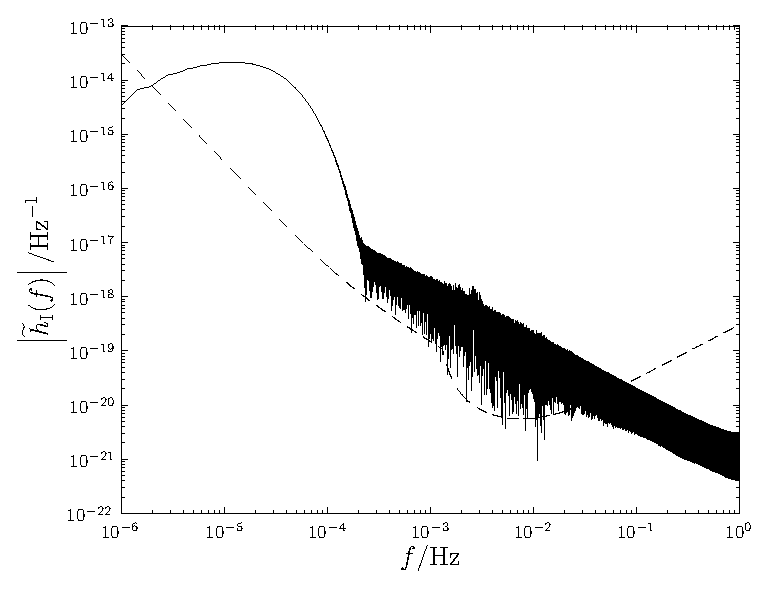
\includegraphics[width=0.45\textwidth]{Fig_h_I_9_rectangular}} \quad
   \subfigure[Spectrum using a Nuttall window. The calculated SNR is $\rho = 8.5$.]{\label{fig:Windowing_Nuttall} 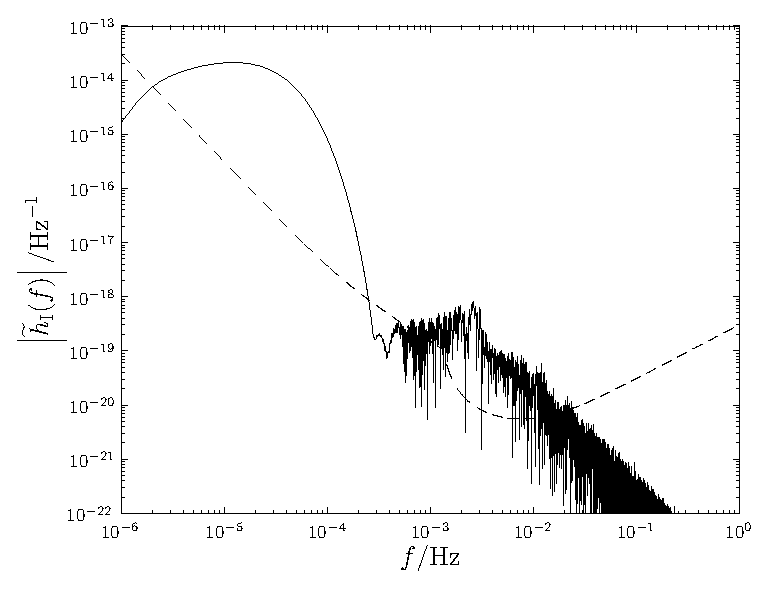
\includegraphics[width=0.45\textwidth]{Fig_h_I_9_Nuttall}}
    \caption{Example spectra calculated using (a) a rectangular window and (b) Nuttall's four-term window with continuous first derivative \citep{Nuttall1981}. The spin of the MBH is $a_\ast = 0.5$, the mass of the orbiting CO is $\mu = 10 M_\odot$, the periapsis is $r\sub{p} = 50 r\sub{g}$ and the inclination is $\iota = 0.1$. The high-frequency tail is the result of spectral leakage. The level of the \textit{LISA} noise curve is indicated by the dashed line. The spectra are from detector I, but the detector II spectra look similar.}
    \label{fig:Windowing}
  \end{center}
\end{figure*}

Despite being many orders of magnitude below the peak level, the high-frequency tail is still well above the noise curve for a wide range of frequencies. It therefore contributes to the evaluation of any inner products, and could mask interesting features. It is possible to reduce the amount of leakage using apodization: to improve the frequency response of a finite time series one can use a weighting window function $w(t)$ which modifies the impulse response in a prescribed way.

The simplest window function is the rectangular (or Dirichlet) window $w\sub{R}(t)$; this is just the top-hat described above. Other window functions are generally tapered.\footnote{When using a tapered window function it is important to ensure that the window is centred upon the signal; otherwise the calculated transform shall have a reduced amplitude.} There is a wide range of window functions described in the literature \citep*{Harris1978,Kaiser1980,Nuttall1981,McKechan2010}. The introduction of a window function influences the spectrum in a manner dependent upon its precise shape. There are two distinct distortions: local smearing due to the finite width of the centre lobe, and distant leakage due to finite amplitude sidelobes. The window function may be optimised such that the peak sidelobe has a small amplitude, or such that the sidelobes decay away rapidly with frequency. Choosing a window function is a trade-off between these various properties, and shall depend upon the particular application.

For use with the parabolic spectra, the primary concern is to suppress the sidelobes. Many windows with good sidelobe behaviour exist; we consider three: the Blackman-Harris minimum four-term window \citep{Harris1978, Nuttall1981}
\begin{equation}
w\sub{BH}(t) = \sum_{n=0}^{3} a\super{BH}_n\cos\left(\frac{2n\pi t}{\tau}\right),
\end{equation}
where
\begin{equation}
\begin{split}
a\super{BH}_0 = 0.35875, \quad a\super{BH}_1 = 0.48829,\\
a\super{BH}_2 = 0.14128, \quad a\super{BH}_3 = 0.01168;
\end{split}
\end{equation}
the Nuttall four-term window with continuous first derivative \citep{Nuttall1981}
\begin{equation}
w\sub{N}(t) = \sum_{n=0}^{3} a\super{N}_n\cos\left(\frac{2n\pi t}{\tau}\right),
\end{equation}
where
\begin{equation}
\begin{split}
a\super{N}_0 = 0.355768, \quad a\super{N}_1 = 0.487396,\\
a\super{N}_2 = 0.144232, \quad a\super{N}_3 = 0.012604,
\end{split}
\end{equation}
and the Kaiser-Bessel window \citep{Harris1978, Kaiser1980}
\begin{equation}
w\sub{KB}(t;\beta) = \frac{I_0\left[\beta\sqrt{1 - (2 t/\tau)^2}\right]}{I_0(\beta)},
\end{equation}
where $I_\nu(z)$ is the modified Bessel function of the first kind, and $\beta$ is an adjustable parameter. Increasing $\beta$ reduces the peak sidelobe, but also widens the central lobe.

The Kaiser-Bessel window has the smallest peak sidelobe, but the worst decay ($1/f$); the Nuttall window has the best asymptotic behaviour ($1/f^3$); the Blackman-Harris window has a peak sidelobe similar to the Nuttall window, and decays asymptotically as fast (slow) as the Kaiser-Bessel window, but has the advantage of having suppressed sidelobes next to the central lobe.

Another window has been recently suggested for use with gravitational waveforms: the Planck-taper window (\citealt*{Damour2000}; \citealt{McKechan2010})
\begin{equation}
w\sub{P}(t; \epsilon) = \begin{cases}
 {\displaystyle \recip{\exp(Z_+)+1}} & {\displaystyle -\frac{\tau}{2} \leq t < -\tau\left(\recip{2} - \epsilon\right)} \\
 1 & {\displaystyle -\tau\left(\recip{2} - \epsilon\right) < t < \tau\left(\recip{2} - \epsilon\right)} \\
 {\displaystyle \recip{\exp(Z_-)+1}} & {\displaystyle -\tau\left(\recip{2} - \epsilon\right) < t \leq \frac{\tau}{2}}
\end{cases},
\end{equation}
with
\begin{equation}
Z_\pm(t; \epsilon) = 2\epsilon\left[\recip{1 \pm 2(t/\tau)} + \recip{1 - 2\epsilon \pm 2(t/\tau)}\right].
\end{equation}
This was put forward for use with binary coalescences, and has superb asymptotic decay. However, the peak sidelobe is high, which is disadvantageous here. We therefore propose a new window function: the Planck-Bessel window which combines the Kaiser-Bessel and Planck-taper windows to produce a window which inherits the best features of both, albeit in a diluted form,
\begin{equation}
w\sub{PB}(t;\beta,\epsilon) = w\sub{P}(t; \epsilon)w\sub{KB}(t;\beta).
\end{equation}
The window functions' frequency responses are plotted in \figref{Response}.
\begin{figure}
  \begin{center}
  \includegraphics[width=0.45\textwidth]{Fig_Response}
    \caption{Window function frequency response. To avoid clutter, the response function is only plotted in detail until $f\tau = 8$, above this a smoothed value is used, as indicated by the dot-dashed line. As well as having good asymptotic behaviour, the Planck-taper window has the narrowest main lobe, except for the rectangular window.}
    \label{fig:Response}
  \end{center}
\end{figure}
There is no window that performs best everywhere.

\Figref{Windowing} shows the computed Fourier transforms for an example EMRB using no window (alternatively a rectangular window), and the Nuttall window.\footnote{The Blackman-Harris, Kaiser-Bessel and Planck-Bessel windows give almost identical results.} Using the Nuttall window, the spectral leakage is greatly reduced; the peak sidelobe is lower, and the tail decays away as $1/{f^3}$ instead of $1/{f}$. The low frequency signal is not appreciably changed.

The choice of window function influences the results as it changes the form of $\widetilde{h}(f)$. The variation in results between windows depends upon the signal: variation is greatest for low frequency bursts, as then there is greatest scope for leakage into the detector frequency band; variation is least significant for zoom-whirl orbits as then there are strong signals to relatively high frequencies, and spectral leakage is confined to mostly below the noise level. To quantify the influence of window functions, we studied the diagonal elements of the Fisher matrix from a selection of orbits with periapses ranging from $\sim 10 r\sub{g}$--$300 r\sub{g}$. For orbits with small periapses all five windows (excluding the rectangular window) produced very similar results: the Planck-taper window differed by a maximum of $\sim 0.5\%$ from the others, which all agreed to better than $0.1\%$. The worst case results came from the lowest frequency orbits, then the Planck-taper window deviated by a maximum of $\sim 30\%$ in the value for the Fisher matrix elements, the Blackman-Harris deviated by $\sim 20\%$ and the others agreed to better than $\sim 5\%$. The Planck-taper window's performance is limited by its poor sidelobe behaviour; the Blackman-Harris has the worst performance at high frequency.

For this work we have used the Nuttall window. Its performance is comparable to the Kaiser-Bessel and Planck-Bessel windows, but it is computationally less expensive to implement as it does not contain Bessel functions. Results should be accurate to a few percent at worst, and results from closer orbits, which provide better constraints, should be less affected by the choice of window function. Therefore, we are confident that none of our conclusions are sensitive to the particular windowing method implemented.

\bsp

\label{lastpage}

\end{document}


\chapter{Parameter estimation and Galactic bursts}\label{ch:param}

EMRBs could provide a means of investigating the properties of MBHs with a space-borne detector. In the previous chapter we constructed approximate burst waveforms. We now begin to investigate their properties. To be useful for astronomy EMRBs must be: (i) detectable, (ii) informative and (iii) likely to happen. If bursts are not detectable, they can be of no use. If they are detectable but not informative, then at best they could only tell us that there are objects on highly eccentric orbits. This could be interesting if we observe enough to do statistics, but this depends upon the event rate. If the event rate is too low, then even if EMRBs are wonderfully informative they are unlikely to be of practical use. EMRBs must fulfill all three criteria to be a viable tool for learning about MBHs.

In this chapter we start to address the first two criteria. We begin by concentrating on the Galaxy's MBH; as it is our local MBH, it is the most promising candidate. In \secref{Waveforms} we look at our NK waveforms and determine that they could be detectable. We give fiducial power law fits for SNR as a function of periapse radius, which are useful for back-of-the-envelope estimates. We explain how to extract the information from the bursts in \secref{Estimation}. Results estimating the measurement precision are then presented in \secref{Gal-Results}.

%In the following chapter we go on to consider extragalactic sources. These are not as promising as the GC, but could still contribute to the total burst event rate. We address the question of event rates in ... where we construct a model for our Galaxy.

\section{Waveforms and detectability}\label{sec:Waveforms}

\subsection{Model parameters}\label{sec:Mod-param}

The waveform depends on the properties of the MBH; the CO and its orbit, and the detector. We assume the position of the detector is known. This is specified by $\overline{\phi}$ and $\varphi$ (see \figref{SS_LISA}). We chose the initial position so $\overline{\phi} = 0$ when $\varphi = 0$ \citep{Cutler1998}; this does not qualitatively influence our results.\footnote{See \citet{Jani2013} for a discussion of the possibilities for optimising the choice of the initial phase.}

We also treat the sky position of the MBH, given by $\overline{\Theta}$ and $\overline{\Phi}$, as known. This is taken to be the location of Sgr A*, as the radio source is expected to be within $20 r\sub{g}$ of the MBH \citep{Reid2003,Doeleman2008}. We use the J2000.0 coordinates \citep{Reid1999, Yusef-Zadeh1999}. These change with time due to the rotation of the SS about the GC; the proper motion is about $6\units{mas\,yr^{-1}}$, mostly in the plane of the Galaxy \citep{Reid1999, Backer1999, Reid2003}. The position is already determined to high accuracy and an EMRB can only give weak constraints on source position, hence we shall not try to infer it.\footnote{For comparison, an EMRI, which should be more informative, can only give sky localisation to $\sim 10^{-3}~\mathrm{steradians}$ \citep{Barack2004, Huerta2009}.}

For our model, the input parameters left to infer are:
\begin{enumerate}[leftmargin=*, widest=\:88--88.]
\item[1.] The MBH's mass $M_\bullet$. This is currently well constrained by the observation of stellar orbits about Sgr A* \citep{Ghez2008, Gillessen2009}, with the best estimate being $M_\bullet = (4.31 \pm 0.36) \times 10^6 M_\odot$. This depends upon the GC distance $R_0$ as $M_\bullet = (3.95 \pm 0.06|\sub{stat} \pm 0.18|_{R_0, \, \mathrm{stat}} \pm  0.31|_{R_0, \, \mathrm{sys}}) \times 10^6 M_\odot (R_0 / 8\units{kpc})^{2.19}$, where the errors are statistical, independent of $R_0$; statistical from the determination of $R_0$, and systematic from $R_0$ respectively.
\item[2.] The spin parameter $a_\ast$. Naively this could be anywhere in the range $|a_\ast| < 1$; however, it is possible to place an upper bound by contemplating spin-up mechanisms. Considering the torque from radiation emitted by an accretion disc, and swallowed by a BH, it can be shown that $|a_\ast| \lesssim 0.998$ \citep{Thorne1974}. Magnetohydrodynamical simulations of accretion discs produce a smaller maximum value of $|a_\ast| \sim 0.95$ \citep{Gammie2004}. The actual spin value could be much lower than this upper bound depending upon the MBH's evolution.
\item[3, 4.] The orientation angles for the MBH spin $\Theta\sub{K}$ and $\Phi\sub{K}$. These are defined in the ecliptic coordinate system from \figref{SS_LISA}.
\item[5.] The ratio of the SS--GC distance $R_0$ and the CO mass $\mu$, which we denote as $\zeta = R_0/\mu$. This scales the amplitude of the waveform. Bursts, unlike inspirals, do not undergo orbital evolution, hence we cannot break the degeneracy in $R_0$ and $\mu$, and they cannot be inferred separately. The distance, like $M_\bullet$, is constrained by stellar orbits, the best estimate being $R_0 = 8.33 \pm 0.35\units{kpc}$ \citep{Gillessen2009}. The mass of the orbiting particle depends upon the type of object: whether it is an MS star, WD, NS or BH. Since we shall not know $\mu$ precisely, we shall not be able to infer anything more about the distance to the GC.
\item[6, 7.] The angular momentum of the CO. This can be described using either $\{L_z, Q\}$ or $\{L_\infty, \iota\}$. We employ the latter, as the total angular momentum and inclination are less tightly correlated. Assuming spherical symmetry, we expect $\cos \iota$ to be uniformly distributed.
\item[8--10.] A set of coordinates to specify the trajectory. These could be positions at an arbitrary time. We use the angular phases at periapse, $\phi\sub{p}$ and $\chi\sub{p}$ (which determines $\theta\sub{p}$), as well as the time of periapse $t\sub{p}$.
\end{enumerate}
We are therefore interested in constraining $d = 10$ parameters. We shall use $\boldsymbol{\lambda}$ to represent the set of these $d$ parameters.

Of paramount importance are the mass and spin. Together, these fully describe the MBH; all the information regarding its formation and growth must be inferred from these parameters. As we have a good estimate of the mass, to gain a complete description of the MBH we have only to measure its spin; this shall give us insight into its history and role in the evolution of the Galaxy.

\subsection{Waveforms and kludge coordinates}\label{sec:wave-ex}

\Figref{Examples} shows example waveforms to demonstrate some of the possible variations in the signal. All these assume the standard mass and position for the MBH as well as a $\mu = 10 M_\odot$ orbiting CO; other (randomly chosen) orbital parameters are specified in the captions. Radii are given in terms of the gravitational radius $r\sub{g} = GM_\bullet / c^2 \simeq 6.36 \times 10^9\units{m}$.
\begin{figure}
  \centering
   \subfigure[{Waveform for $a_\ast \simeq 0.12$, $r\sub{p} \simeq 15.6 r\sub{g}$ and $\iota \simeq 2.1$. The SNR for the spherical polar kludge waveform (plotted) is $\rho[\boldsymbol{h}\sub{sph}] \simeq 451$, for the oblate-spheroidal kludge it is $\rho[\boldsymbol{h}\sub{ob}] \simeq 451$ (agreement to $0.01\%$).}]{\label{fig:Orbit_233} \includegraphics[width=0.47\textwidth]{./images/Fig_new_sph_h_233}} \quad
   \subfigure[{Waveform for $a_\ast \simeq 0.74$, $r\sub{p} \simeq 3.2 r\sub{g}$ and $\iota \simeq 1.2$. The SNR for the spherical polar kludge waveform (plotted) is $\rho[\boldsymbol{h}\sub{sph}] \simeq 70600$, for the oblate-spheroidal kludge it is $\rho[\boldsymbol{h}\sub{ob}] \simeq 74900$.}]{\label{fig:Orbit_135} \includegraphics[width=0.47\textwidth]{./images/Fig_new_sph_h_135}}  
\caption{Example burst waveforms from the GC. The strain $\widetilde{h}\sub{I}(f)$ is indicated by the solid line, $\widetilde{h}\sub{II}(f)$ by the dot--dashed line, and the noise curve by the dashed line. The kludge has been formulated using spherical polar coordinates.}
  \label{fig:Examples}
\end{figure}

The plotted waveforms use the spherical polar coordinate system for the NK. Using oblate-spheroidal coordinates makes a small difference. On the scale shown here the only discernible difference would be in \figref{Orbit_135}; the maximum difference in that waveform (outside the high-frequency tail) is $\sim 10\%$. In the other cases the difference is entirely negligible (except in the high-frequency tail, which is not of physical significance). This behaviour is typical; for the closest orbits, with the most extreme spin parameters, the maximum difference in the waveforms may be $\sim 30\%$. The difference is largely confined to the higher frequency components, which are most sensitive to the parts of the trajectory closer to the MBH: the change in flat-space radius for the same Boyer--Lindquist radial coordinate causes a slight shift in the shape of the spectrum. Enforcing the same flat-space periapsis gives worse agreement across the spectrum.

To examine the effect of the coordinate choice, we compare SNRs calculated using the alternative schemes for a selection of orbits. The orbits have periapse distances uniformly distributed in logarithmic space between the innermost orbit and $100 r\sub{g}$. Each had a spin and orbital inclination randomly chosen from distributions uniform in $a_\ast$ and $\cos \iota$.\footnote{The innermost orbit depends upon $a_\ast$ and $\iota$, hence these are drawn first.} For every periapse, five SNRs were calculated, each having a different set of ancillary parameters specifying the relative orientation of the MBH, the orbital phase, and the position of the detector, drawn from appropriate uniform distributions. We take the mean of $\ln \rho$ for each set of ancillary parameters.\footnote{The logarithm is a better quantity to work with since the SNR is a positive-definite quantity that may be distributed over a range of magnitudes \citep[sections 22.1, 23.3]{MacKay2003}. Using median values yields results that are quantitatively similar.} The MBH parameters were fixed as for the GC.

The ratio of the two SNRs is shown in \figref{Oblate_sphere}. 
The difference from the coordinate systems is only apparent for orbits with very small periapses. There is agreement to $10\%$ down to $r\sub{p} \simeq 4 r\sub{g}$; the maximal difference may be expected to be $\sim 20\%$, this is for periapses that are only obtainable for high spin values.
\begin{figure}
\centering
 \includegraphics[width=0.6\textwidth]{./images/Fig_SNR_ratio}
 \caption{Ratio of SNR for a waveform calculated using spherical polar coordinates to that for a waveform using oblate-spheroidal coordinates.}
   \label{fig:Oblate_sphere}
\end{figure}

Since the deviation in the two waveforms is only apparent for small periapses, when the kludge approximation is least applicable, we conclude that the choice of coordinates is unimportant. The potential error of order $10\%$ is no greater than that inherent in the NK approximation (see \secref{Energy}). Without an accurate waveform template to compare against, we do not know if there is a preferable choice of coordinates. We adopt spherical coordinates for easier comparison with existing work.

\subsection{Signal-to-noise ratios}\label{sec:Gal-SNR}

The detectability of a burst depends upon its SNR. To characterise the variation of $\rho$ we calculated SNRs for a range of orbits. These were generated as in \secref{wave-ex}; we used $\sim 10^4$ different periapse distances.

The bursts were calculated for a $1 M_\odot$ CO. From \eqnref{octupole}, the amplitude of the waveform is proportional to the CO mass $\mu$, and so $\rho$ is also proportional to $\mu$; a $10 M_\odot$ object would be ten times louder on the same orbit. To make results mass independent, we work in terms of a mass-normalised SNR
\begin{equation}
\hat{\rho}[\boldsymbol{h}] = \left(\dfrac{\mu}{M_\odot}\right)^{-1}\rho[\boldsymbol{h}].
\end{equation}

There exists a correlation between the periapse radius and SNR, as shown in \figref{SNR}. 
\begin{figure}
  \centering
  \includegraphics[width=0.6\textwidth]{./images/Fig_SNR}
    \caption{Mass-normalised SNR as a function of periapse radius for LISA. The plotted points are the values obtained by averaging over each set of ancillary parameters. The best fit line is $\log(\hat{\rho}) = -2.69\log(r\sub{p}/r\sub{g}) + 4.88$. This is fitted to orbits with $r\sub{p} >  13.0 r\sub{g}$.} % and has a reduced chi-squared value of $\chi^2/\nu = 1.73$
  \label{fig:SNR}
\end{figure}
Closer orbits produce louder bursts. To reflect this trend, we have fitted a simple fiducial power law,
\begin{equation}
%\log\rho \simeq -2.7\log\left(\dfrac{r\sub{p}}{r\sub{g}}\right) + \log\left(\dfrac{\mu}{M_\odot}\right) + 4.9,
\log\widehat{\rho} \simeq -2.7\log\left(\dfrac{r\sub{p}}{r\sub{g}}\right) + 4.9,
\label{eq:SNR-power-law}
\end{equation}
which is indicated by the straight line.\footnote{Using oblate-spheroidal coordinates instead of spherical polars gives a fit consistent to within $0.1\%$ as we have excluded the closest orbits.} This was done by maximising the likelihood, assuming $\ln \rho$ has a Gaussian distribution with standard deviation derived from the scatter caused by variation of the ancillary parameters. The power law is a good fit only for larger periapses. The shape is predominately determined by the noise curve. The change in the trend reflects the transition from approximately power law behaviour to the bucket of the noise curve. Hence, we fit a power law to orbits with a characteristic frequency of $f_\ast = \sqrt{GM_\bullet/r\sub{p}} < 1 \times 10^{-3}\units{Hz}$, to avoid spilling into the bucket.\footnote{The form of $f_\ast$ can be derived on dimensional grounds and is explained in more detail in \secref{extragal-SNR}.} Changing the cut-off within a plausible region alters the fit coefficients by around $0.1$.\footnote{The power law exponent $-2.7$ is inconsistent with $-13/4$ as predicted by the approximate model of \citet{Hopman2007}. This is the result of their approximate waveform model.}

The SNR shows no clear correlation with the other parameters (excluding $\mu$). However, the SNR is sensitive to the orbital parameters, in particular the periapse phases $\chi\sub{p}$ and $\phi\sub{p}$, and may vary by an order of magnitude.

Setting a threshold of $\rho = 10$, a $1 M_\odot$ ($10 M_\odot$) CO burst would be expected to be detectable if the periapse distance is less than $27 r\sub{g}$ ($65 r\sub{g}$). \citet{Hopman2007}, assuming a threshold of $\rho = 5$, used an approximate form for the SNR based upon the quadrupole component of a circular orbit; their model, with updated parameters for the MBH, predicts bursts would be detectable out to $66 r\sub{g}$ ($135 r\sub{g}$). This is overly optimistic.

Following a similar approach, we may repeat this analysis for eLISA. The SNR as a function of periapse is shown in \figref{SNR-eLISA}.
\begin{figure}
  \centering
  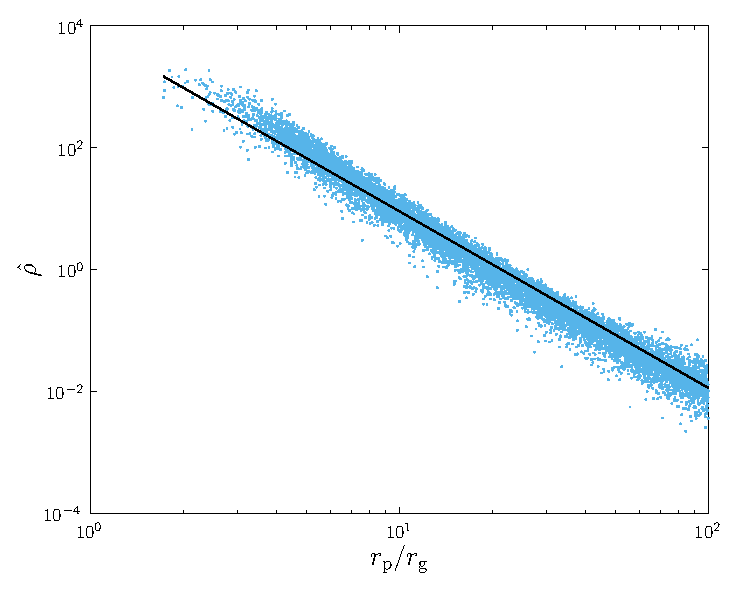
\includegraphics[width=0.6\textwidth]{./images/Fig_SNR_eLISA_NGO}
    \caption{Mass-normalised SNR as a function of periapse radius for eLISA. The plotted points are the values obtained by averaging over each set of ancillary parameters. The best fit line is $\log(\hat{\rho}) = -2.90\log(r\sub{p}/r\sub{g}) + 3.85$. This is fitted to orbits with $r\sub{p} >  13.0 r\sub{g}$.}
    \label{fig:SNR-eLISA}
\end{figure}
There is again a strong correlation that may be approximated as a power law. The bucket of the noise curve is less apparent as it is shifted to slightly higher frequencies. We have fitted
\begin{equation}
%\log\rho \simeq -2.9\log\left(\dfrac{r\sub{p}}{r\sub{g}}\right) + \log\left(\dfrac{\mu}{M_\odot}\right) + 3.9,
\log\rho \simeq -2.9\log\left(\dfrac{r\sub{p}}{r\sub{g}}\right) + 3.9,
\label{eq:SNR-power-law-eLISA}
\end{equation}
which is indicated by the straight line. This was done in exactly the same way as for LISA. Again, there is no clear correlation with any other orbital parameters.

The SNR is lower for eLISA. As a consequence, bursts are detectable across a smaller range of periapses. Using the threshold $\rho = 10$, a $1 M_\odot$ ($10 M_\odot$) CO burst would be expected to be detectable if the periapse distance is less than $10 r\sub{g}$ ($21 r\sub{g}$). This is a reduction of about a factor of three compared to LISA.

\section{Parameter estimation}\label{sec:Estimation}

Having detected a signal, we are interested in what we can learn about the source. We have an inference problem that can be solved by an application of Bayes' Theorem \citep[chapter 4]{Jaynes2003}: the probability distribution for our parameters given that we have detected the signal $\boldsymbol{s}(t)$ is given by the posterior
\begin{equation}
p(\boldsymbol{\lambda}|\boldsymbol{s}(t)) = \dfrac{p(\boldsymbol{s}(t)|\boldsymbol{\lambda})p(\boldsymbol{\lambda})}{p(\boldsymbol{s}(t))}.
\end{equation}
Here $p(\boldsymbol{s}(t)|\boldsymbol{\lambda})$ is the likelihood of the parameters, $p(\boldsymbol{\lambda})$ is the prior probability distribution for the parameters, and the evidence $p(\boldsymbol{s}(t)) = \intd{}{}{p(\boldsymbol{s}(t)|\boldsymbol{\lambda})}{^d \lambda}$ is, for our purposes, a normalising constant. The likelihood depends upon the realisation of noise. If parameters $\boldsymbol{\lambda}_0$ define a waveform $\boldsymbol{h}_0(t) = \boldsymbol{h}(t; \boldsymbol{\lambda}_0)$, the probability that we observe signal $\boldsymbol{s}(t)$ GW is given by \eqnref{sig_prob}, so the likelihood is
\begin{equation}
p(\boldsymbol{s}(t)|\boldsymbol{\lambda}_0) \propto \exp\left[-\recip{2}\innerprod{\boldsymbol{s}-\boldsymbol{h}_0}{\boldsymbol{s}-\boldsymbol{h}_0}\right].
\label{eq:likelihood}
\end{equation}
If we were to define this as a probability distribution for the parameters $\boldsymbol{\lambda}$, the modal values are the maximum-likelihood (ML) parameters $\boldsymbol{\lambda}\sub{ML}$. The waveform $\boldsymbol{h}(t; \boldsymbol{\lambda}\sub{ML})$ is the signal closest to $\boldsymbol{s}(t)$, where distance is defined using the inner product (\ref{eq:inner}) \citep{Cutler1994}.

To discover if any parameters can be accurately inferred, we must characterise the form of the posterior. We discuss two approaches for mapping the shape of the posterior: Fisher matrices and Markov chain Monte Carlo (MCMC) sampling.

\subsection{Fisher information matrices}\label{sec:Fisher}

In the limit of a high SNR, we may approximate \citep{Vallisneri2008}
\begin{equation}
p(\boldsymbol{s}(t)|\boldsymbol{\lambda}_0) \propto \exp\left[-\recip{2}\innerprod{\partial_a\boldsymbol{h}}{\partial_b\boldsymbol{h}}\left(\lambda^a - \langle\lambda^a\rangle_\ell\right)\left(\lambda^b - \left\langle\lambda^b\right\rangle_\ell\right)\right],
\label{eq:LSA}
\end{equation}
where the mean is defined as
\begin{equation}
\langle\lambda^a\rangle_\ell = \dfrac{\intd{}{}{\lambda^a p(\boldsymbol{s}(t)|\boldsymbol{\lambda})}{^d \lambda}}{\intd{}{}{p(\boldsymbol{s}(t)|\boldsymbol{\lambda})}{^d \lambda}}.
\end{equation}
In the high SNR limit, this is the ML value $\langle\lambda^a\rangle_\ell = \lambda^a\sub{ML}$. The quantity
\begin{equation}
\Gamma_{ab} = \innerprod{\partial_a\boldsymbol{h}}{\partial_b\boldsymbol{h}}
\label{eq:Fisher}
\end{equation}
is the Fisher information matrix (FIM). It controls the variance of the likelihood distribution.

The form of the posterior distribution depends upon the nature of the prior information. If we have an uninformative prior, such that $p(\boldsymbol{\lambda})$ is a constant, the posterior distribution is determined by the likelihood. In the high SNR limit, we obtain a Gaussian with variance--covariance matrix
\begin{equation}
\boldsymbol{\Sigma} = \boldsymbol{\Gamma}^{-1}.
\label{eq:InvFisher}
\end{equation}
The FIM therefore gives the uncertainty associated with the inferred parameters, in this case the ML values.

If the prior restricts the allowed range for a parameter, as is the case for the spin $a_\ast$, then the posterior is a truncated Gaussian, and $\boldsymbol{\Gamma}^{-1}$ may no longer represent the variance--covariance.

If the prior is approximately Gaussian with variance--covariance matrix $\boldsymbol{\Sigma}_0$, the posterior is also Gaussian.\footnote{If we only know the typical value and spread of a parameter, a Gaussian is the maximum entropy prior (\citealt{Jaynes2003}, section 7.11): the prior that is least informative given what we know.} The posterior variance--covariance is \citep{Cutler1994, Vallisneri2008}
\begin{equation}
\boldsymbol{\Sigma} = \left(\boldsymbol{\Gamma} + \boldsymbol{\Sigma}_0^{-1}\right)^{-1}.
\label{eq:Posterior_variance}
\end{equation}
From this the inverse FIM $\boldsymbol{\Gamma}^{-1}$ is an upper bound on the size of the posterior covariance matrix.\footnote{It is also the Cram\'{e}r-Rao bound on the error covariance of an unbiased estimator \citep{Cutler1994, Vallisneri2008}. Thus it represents the frequentist error: the lower bound on the covariance for an unbiased parameter estimator $\boldsymbol{\lambda}\sub{est}$ calculated from an infinite set of experiments with the same signal $\boldsymbol{h}(t)$ but different realisations of the noise $\boldsymbol{n}(t)$.}

The FIM gives a quick way of estimating the range of the posterior. It is widely used because of this. However, it is only appropriate when the approximation of \eqnref{LSA} holds. This is known as the linearised-signal approximation (LSA), where higher order derivatives are neglected. To assess the validity of this, \citet{Vallisneri2008} recommends use of the maximum-mismatch (MM) criterion
\begin{equation}
\ln r = -\recip{2}\innerprod{\Delta\lambda^a\partial_a\boldsymbol{h}\sub{ML} - \Delta\boldsymbol{h}}{\Delta\lambda^b\partial_b\boldsymbol{h}\sub{ML} - \Delta\boldsymbol{h}}.
\end{equation}
Here $\Delta \boldsymbol{\lambda}$ is the displacement to some point on the $1\sigma$ surface
\begin{equation}
\Delta \boldsymbol{\lambda} = \boldsymbol{\lambda}\sub{1\sigma} - \boldsymbol{\lambda}\sub{ML},
\end{equation}
and $\Delta \boldsymbol{h}$ is the corresponding change in the waveform
\begin{equation}
\Delta \boldsymbol{h} = \boldsymbol{h}(\boldsymbol{\lambda}\sub{1\sigma}) - \boldsymbol{h}(\boldsymbol{\lambda}\sub{ML}).
\end{equation}
The $1\sigma$ surface is defined from the inverse of the FIM. If higher order terms are indeed negligible, the MM criterion is small. We check this by picking a random selection of points on the $1\sigma$ surface and evaluating $|\ln r|$. If this is smaller than a fiducial value ($|\ln r| = 0.1$) over the majority ($90\%$) of the surface we consider the LSA sufficiently justified.

We calculated FIMs for a wide range of orbits and checked the MM criterion. We found that for the overwhelming majority the test failed: the LSA is not appropriate. This behaviour was seen even for orbits with $\rho \sim 10^3$--$10^4$.\footnote{In this study, to increase $\rho$ we must reduce the periapse distance; this also reduces the region where the LSA is valid as parameter dependencies become more non-linear. If we had the luxury of increasing $\rho$ by moving the GC closer, things could be different.} Higher order terms are important, and cannot be neglected.

EMRBs have a short duration and accordingly are not the most informative of signals. Therefore, the $1\sigma$ surface as defined by considering only the LSA terms is large. Taking such a step in parameter space moves the signal beyond the region of linear changes.

What constitutes high SNR depends upon the signal; it is not enough for $\rho > 1$. As stressed by \citet{Vallisneri2008}, it is essential to check the MM criterion for individual waveforms: the threshold for the LSA to become applicable could be much greater than naively thought.

As we cannot be confident in FIM results, we abandon this approach in favour of using MCMC simulations to explore constraints from different regions of parameter space. These are computationally more expensive, but do not rely on any approximations.

\subsection{Markov chain Monte Carlo methods}\label{sec:MCMC}

MCMC methods are widely used for inference problems; they are a family of algorithms for integrating over complicated distributions and are efficient for high-dimensional problems \citep[chapter 29]{MacKay2003}. Parameter space is explored by constructing a chain of $N$ samples. The distribution of points visited by the chain maps out the underlying distribution; this becomes asymptotically exact as $N \rightarrow \infty$. Samples are added sequentially, if the current state is $\boldsymbol{\lambda}_n$ a new point $\boldsymbol{\lambda}^\ast$ is drawn and accepted with probability
\begin{equation}
\mathcal{A} = \min\left\{\dfrac{\pi(\boldsymbol{\lambda}^\ast)\mathcal{L}(\boldsymbol{\lambda}^\ast)\mathcal{Q}(\boldsymbol{\lambda}_n;\,\boldsymbol{\lambda}^\ast)}{\pi(\boldsymbol{\lambda}_n)\mathcal{L}(\boldsymbol{\lambda}_n)\mathcal{Q}(\boldsymbol{\lambda}_n;\,\boldsymbol{\lambda}^\ast)}, 1\right\},
\end{equation}
setting $\boldsymbol{\lambda}_{n + 1} = \boldsymbol{\lambda}^\ast$, where $\mathcal{L}(\boldsymbol{\lambda})$ is the likelihood, in our case from \eqnref{likelihood}; $\pi(\boldsymbol{\lambda})$ is the prior, and $\mathcal{Q}$ is a proposal distribution. If the move is not accepted  $\boldsymbol{\lambda}_{n + 1} = \boldsymbol{\lambda}_n$. This is the Metropolis--Hastings algorithm \citep{Metropolis1953,Hastings1970}.

Waiting long enough yields an exact posterior, but it is desirable for the MCMC to converge quickly. This requires a suitable choice for the proposal distribution, which can be difficult, since we do not yet know the shape of the target distribution.

One method to define the proposal is to use the previous results in the chain and refine $\mathcal{Q}$ by learning from these. Such approaches are known as adaptive methods. Updating using previous points means that the chain is no longer Markovian. Care must be taken to ensure that ergodicity is preserved and convergence obtained \citep{Roberts2007,Andrieu2008}. To avoid this complication, we follow \citet{Haario1999}, and use the adapting method as a burn in phase. We have an initial phase where the proposal is updated based upon accepted points. After this we fix the proposal and proceed as for a standard MCMC. By only using samples from the second part, we guarantee that the chain is Markovian and ergodic, whilst still enjoying the benefits of a tailor-made proposal. After only a finite number of samples we cannot assess the optimality of this \citep{Andrieu2008}, but the method is still effective.

To tune $\mathcal{Q}$, we use an approach based upon the adaptive Metropolis algorithm \citep{Haario2001}. The proposal is taken to be a multivariate Gaussian distribution centred upon the current point, the covariance of which is
\begin{equation}
\boldsymbol{C} = s \left(\boldsymbol{V}_n + \varepsilon\boldsymbol{C}_0\right),
\end{equation}
where $\boldsymbol{V}_n$ is the covariance of the accepted points $\{\boldsymbol{\lambda}_1,\ldots,\boldsymbol{\lambda}_n\}$, $s$ is a scaling factor that controls the step size, $\varepsilon$ is a small positive constant (typically $2.5 \times 10^{-3}$), and $\boldsymbol{C}_0$ is a constant matrix included to ensure ergodicity.

Our adaptation is run in three phases. The initial phase is to get the chain moving. For this, $\boldsymbol{C}_0\super{init}$ is a diagonal matrix with elements calibrated from initial one-dimensional MCMCs. This finishes after $N\sub{init}$ accepted points.

For the second phase, we use the proposal covariance from the initial phase $\boldsymbol{C}\super{init}$ for $\boldsymbol{C}_0\super{main}$. We reset the covariance of the accepted points so that it only includes points from this phase. This is the main adaptation phase and lasts until $N\sub{main}$ points have been accepted.

In the final adaptation phase we restart the chain at the true parameter values. We no longer update the shape of the covariance ($\boldsymbol{V}_n$ remains fixed), but adjust the step size $s$ to tune the acceptance rate; it is then fixed, along with everything else, for the final MCMC.

Throughout the adaptation, we update the step size $s$ after every $100$ trial points (whether or not they are accepted). While updating, the covariance $\boldsymbol{V}_n$ changes after every $10^3$ trial points. We set $N\sub{init} = 5 \times 10^4$ and $N\sub{main} = 4.5 \times 10^5$.

We initially aimed for an acceptance rate of $0.234$; this is optimal for a random walk Metropolis algorithm with some specific high-dimensional target distributions \citep{Roberts1997,Roberts2001}. In many cases we found better convergence when aiming for a lower acceptance rate, say $0.1$. This is not unexpected: the optimal rate may be lower than $0.234$ when the parameters are not independent and identically distributed \citep{Bedard2007, Bedard2008a, Bedard2008}. In practice, the final acceptance rate is (almost always) lower than the target rate as the use of a multivariate Gaussian for the proposal distribution is rarely a good fit at the edges of the posterior. Consequently, the precise choice for the target acceptance rate is unimportant as long as it is of the correct magnitude. Final rates are typically within a factor of two of the target value. As an initial choice, we set $s = 2.38^2/d$, which is the optimal choice if $\boldsymbol{C}$ was the true target covariance for a high-dimensional target of independent and identically distributed parameters \citep{Gelman1996,Roberts1997,Roberts2001,Haario2001}.\footnote{Reasonably good results may be obtained by fixing $s$ at this value, and not adjusting to fine-tune the acceptance rate.}

To assess the convergence of the MCMC we check the trace plot (the parameters' values throughout the run) for proper mixing, that the one- and two-dimensional posterior plots fill out to a smooth distribution, and that the distribution widths tend towards consistent values.

\section{Results for Galactic bursts}\label{sec:Gal-Results}

To asses the utility of EMRBs for parameter estimation, we studied bursts from a range of orbits with periapses uniformly distributed in logarithmic space between the the inner-most orbit and $16 r\sub{g}$. Parameters were chosen as in \secref{wave-ex}. The MBH was assumed to have the standard mass and position and the CO was chosen to be $10 M_\odot$, as the most promising candidates for EMRBs would be BHs: they are massive and hence produce higher SNR bursts, they are more likely to be on close orbits as a consequence of mass segregation \citep{Bahcall1977, Alexander2009}, and they cannot be tidally disrupted.

The results of the MCMC runs show strong and complex parameter dependencies. Some example results are shown in figures \ref{fig:MCMC-1}, \ref{fig:MCMC-2} and \ref{fig:MCMC-3}.
\begin{figure}
\centering
\vspace{0.5\baselineskip}
   \includegraphics[width=0.8\textwidth]{./images/Fig_MCMC_327_triangle_40}
\caption{Marginalised one- and two-dimensional posteriors (on the diagonal and above, respectively). The scales are identical in both sets of plots. The dotted line indicates the true value. These distributions are fairly cromulent and well converged. Angular momentum is in units of $L_\bullet = GM_\bullet c^{-1}$  and the scaled distance is in units of $\zeta_0 = 1 M_\odot^{-1}\units{kpc}$. The input orbit has $r\sub{p} \simeq 8.54 r\sub{g}$ and $\rho \simeq 916$.}
\label{fig:MCMC-1}
\end{figure}
The first is well-behaved. It is almost Gaussian, but we see some asymmetries and imperfections. There are also strong degeneracies, indicated by needle-like distributions. This is a fairly standard example: there are runs which are closer to being Gaussian (especially at higher SNR), and equally there are tighter correlations. The lenticular $M_\bullet$--$L_\infty$ degeneracy is common.

\begin{figure}
\centering
\vspace{0.5\baselineskip}
   \includegraphics[width=0.8\textwidth]{./images/Fig_MCMC_53_triangle_40}
\caption{Marginalised one- and two-dimensional posteriors. The conventions are the same as in \figref{MCMC-1}. These distributions show definite non-gaussianity. The input orbit has $r\sub{p} \simeq 9.86 r\sub{g}$ and $\rho \simeq 1790$.}
\label{fig:MCMC-2}
\end{figure}
The second shows banana-like degeneracies. These are not uncommon; there are varying degrees of curvature. The more complicated shape makes it harder for the MCMC to converge, so the final distribution is not as smooth as for the first example. The curving degeneracies also bias the one-dimensional marginalisations away from the true values.

\begin{figure}
\centering
\vspace{0.5\baselineskip}
   \includegraphics[width=0.8\textwidth]{./images/Fig_MCMC_181_triangle_40}
\caption{Marginalised one- and two-dimensional posteriors. The conventions are the same as in \figref{MCMC-1}. These distributions show complicated degeneracies. The input orbit has $r\sub{p} \simeq 11.60 r\sub{g}$ and $\rho \simeq 590$.}
\label{fig:MCMC-3}
\end{figure}
The third shows more intricate behaviour. This is more rare, but indicates the variety of shapes that is obtainable. Again the convergence is more difficult, so the distributions are rougher around the edges; there is also some biasing due to the curving degeneracies.

Our results do not incorporate any priors (save to keep them within realistic ranges); we have not folded in the existing information we have, for example, about the MBH's mass. Therefore, the resulting distributions characterise what we could learn from EMRBs alone. By the time a space-borne GW detector finally flies, we will have much better constraints on some parameters.

It is possible to place good constraints from the closest orbits. These can provide sufficient information to give beautifully behaved posteriors although significant correlation between parameters persists.

\subsection{Distribution widths}

\subsubsection{Characterising distributions}\label{sec:k-d}

Having recovered the posterior distribution it is necessary to quantify the accuracy to which parameters could be measured. If the posterior were Gaussian, this can be done just by using the standard deviation $\sigma\sub{SD}$. An alternative is to use the range that encloses a given probability, but this is misleading if the distribution is multimodal. A robust means of characterising the width is by using a $k$-dimensional ($k$-d) tree.

A $k$-d tree is a type of binary space partitioning tree \citep[sections 5.2, 12.1, 12.3]{Berg2008}. It is constructed by splitting the parameter space into two by finding the median point in one dimension. The two pieces are then split by finding their medians in another dimension. This continues recursively until the desired number of partitions, known as leaves, has been created. When applied to a sampled probability distribution, a $k$-d tree has smaller leaves in the regions of high probability which are of most interest \citep{Weinberg2012}. It builds a natural decomposition of the parameter space, giving a means of binning samples.

For a given probability $p$, the corresponding confidence region is the smallest area of parameter space in which we expect that the true values lie with that probability. A simple means of constructing a confidence range is to find the smallest combination of $k$-d tree leaves that contain the desired probability. To do this we rank the leaves by size; the smallest corresponds to the highest probability area and is the starting point for the confidence range. We continue adding the next smallest leaf until the total probability enclosed is $p$. Summing the areas of the leaves gives an estimate for the range.

However, this approach is biased. Whenever a random fluctuation in the sampling gives an excess of points in one area the overdensity leads to a smaller leaf size and then the preferential inclusion of that leaf in the confidence interval. Conversely, an underdensity leads to a larger leaf that is liable to be external to the confidence range. If there are a small number of points per leaf we shall overstate our confidence as the constructed range is too small.\footnote{This can be visualised by considering the simple example of dividing in two samples from a one-dimensional uniform distribution. We would expect one partition to be more densely populated than the other because of random fluctuations, and we shall always pick this smaller leaf as our $p = 0.5$ confidence range. As the number of points increases we expect that this bias would decrease.}

Biasing may be avoided by using a two-step method which separates the creation and ordering of the partitions from the building of the confidence range \citep{Sidery2013}. This is done by dividing our data into two disjoint random samples.\footnote{We split our data into two equal parts. This may not be the optimal rationing, but is a sensible first guess. Some preliminary experimentation shows that it is not too important, provided that the splitting is not too unbalanced. The point at which this occurs depends upon the underlying distribution.} The first is used to construct the $k$-d tree in the standard way. The leaves are then ordered by size. We then use the second set to populate the leaves. We again start with the smallest leaf and work down the ranking until the encompassed probability is $p$. The total range is the estimate for the $p$ confidence level.

The first step creates bins that are of appropriate resolution. We therefore have the benefit of using a $k$-d tree. By using an independent set of points to build the confidence level, we eliminate any bias because there should be no correlation in fluctuations between the two sets. Any leaves that are too small are expected to receive a below average number of points in the second step and any that are too large are expected to receive more. This corrects the expectation for the confidence level.

In this case, we are interested in the confidence levels for the marginalised distributions for each parameter. We therefore construct $1$-d trees, which are easily implemented. We have a large number of points and low dimensionality, so biasing should not be an issue. To characterise our distributions we find the $p = 0.68$ confidence range and take the half-width of this, which we denote as $\sigma_{0.68}$.

\subsubsection{Parameter uncertainties}

Characteristic distribution widths $\sigma\sub{SD}$ and $\sigma_{0.68}$ are shown in \figref{sigmas}. Filled circles are used for runs that appear to have converged. Open circles are for those yet to converge, but which appear to be approaching an equilibrium state; widths should be accurate to within a factor of a few.
\begin{figure}%[htp]
\centering
\subfigure[MBH mass $M_\bullet$ versus periapsis.]{\includegraphics[width=0.475\textwidth]{./images/Fig_MW_MCMC_sigmas_rp_1}} \quad
\subfigure[MBH mass $M_\bullet$ versus SNR.]{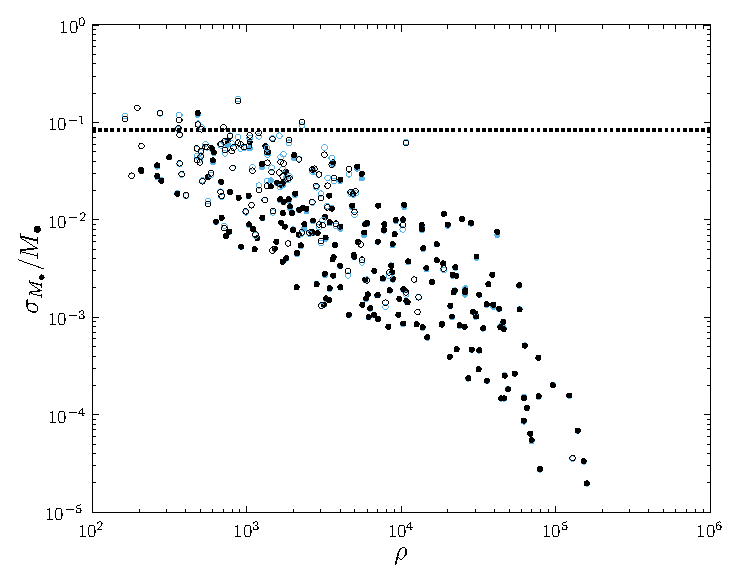
\includegraphics[width=0.485\textwidth]{./images/Fig_MW_MCMC_sigmas_SNR_1}} \\
\subfigure[MBH spin $a_\ast$ versus periapsis.]{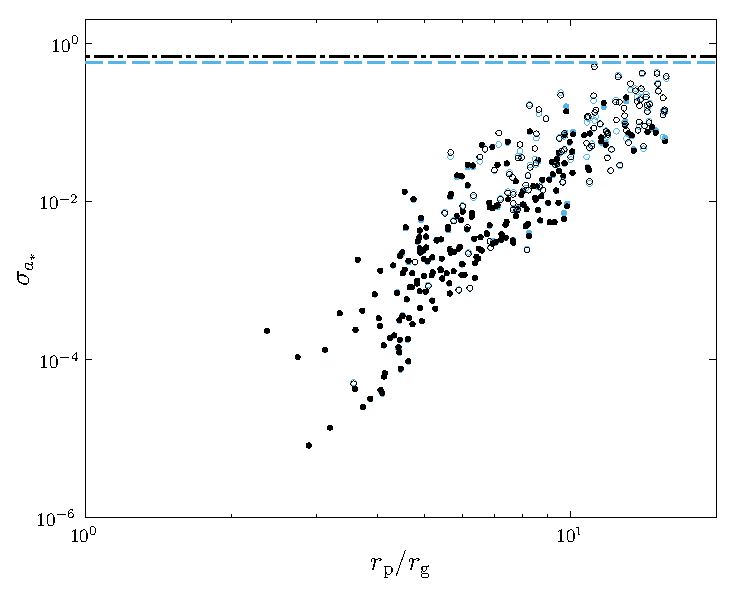
\includegraphics[width=0.475\textwidth]{./images/Fig_MW_MCMC_sigmas_rp_2}} \quad
\subfigure[MBH spin $a_\ast$ versus SNR.]{\includegraphics[width=0.485\textwidth]{./images/Fig_MW_MCMC_sigmas_SNR_2}} \\
\subfigure[Orientation angle $\Theta\sub{K}$ versus periapsis.]{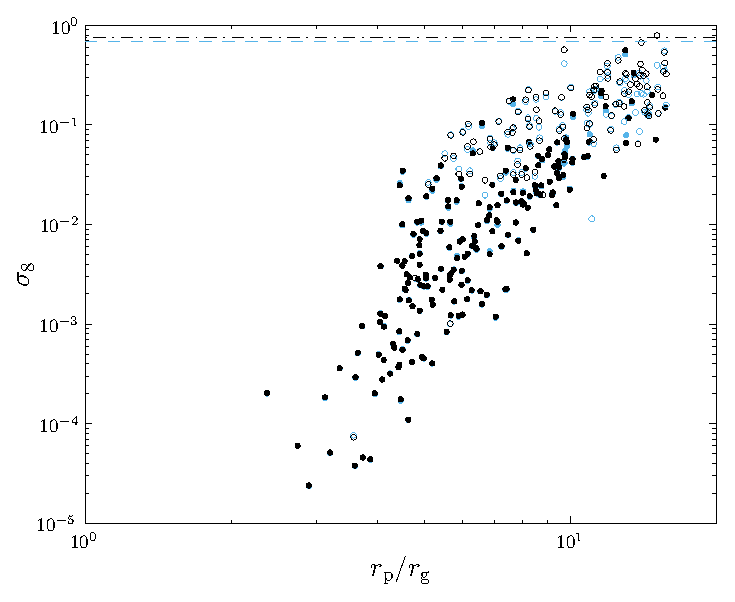
\includegraphics[width=0.475\textwidth]{./images/Fig_MW_MCMC_sigmas_rp_8}} \quad
\subfigure[Orientation angle $\Theta\sub{K}$ versus SNR.]{\includegraphics[width=0.485\textwidth]{./images/Fig_MW_MCMC_sigmas_SNR_8}}
\caption{Distribution widths as functions of periapsis $r\sub{p}$ and SNR $\rho$. The light blue points are used for the standard deviation, the black for the $68$-percentile half-width. The filled circles are converged runs and the open circles for those yet to converge. The dotted line is the current uncertainty for $M_\bullet$. The dashed line is the standard deviation for an uninformative prior and the dot--dashed line is the equivalent $68$-percentile half-width.}
\label{fig:sigmas}
\end{figure}
\begin{figure}%[htp]
\setcounter{subfigure}{6}
\centering
\subfigure[Orientation angle $\Phi\sub{K}$ versus periapsis.]{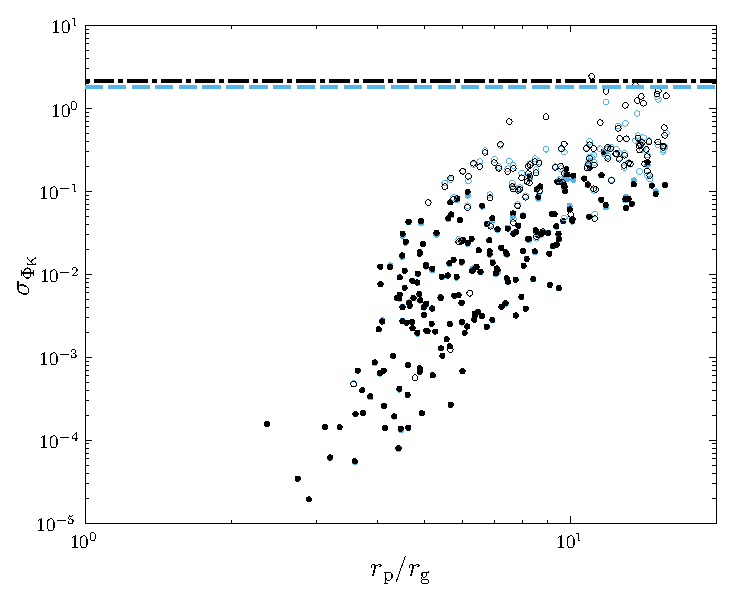
\includegraphics[width=0.475\textwidth]{./images/Fig_MW_MCMC_sigmas_rp_9}} \quad
\subfigure[Orientation angle $\Phi\sub{K}$ versus SNR.]{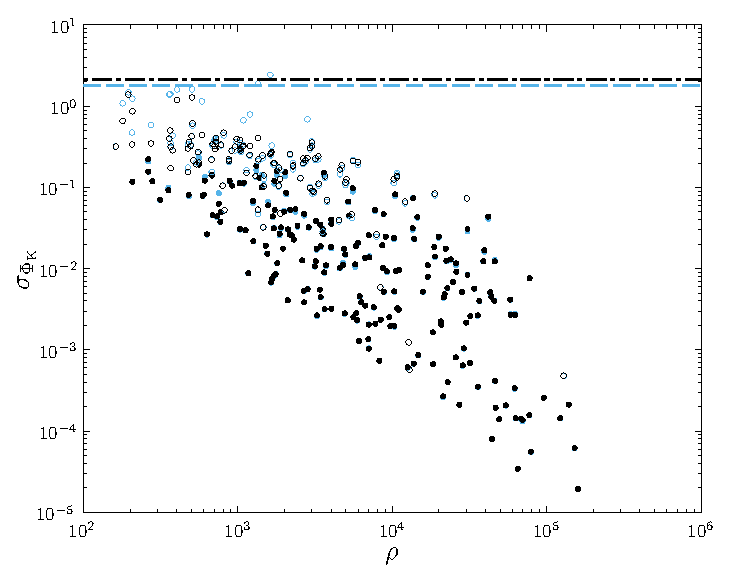
\includegraphics[width=0.485\textwidth]{./images/Fig_MW_MCMC_sigmas_SNR_9}} \\
\subfigure[Scaled distance $\zeta$ versus periapsis.]{\includegraphics[width=0.475\textwidth]{./images/Fig_MW_MCMC_sigmas_rp_10}} \quad
\subfigure[Scaled distance $\zeta$ versus SNR.]{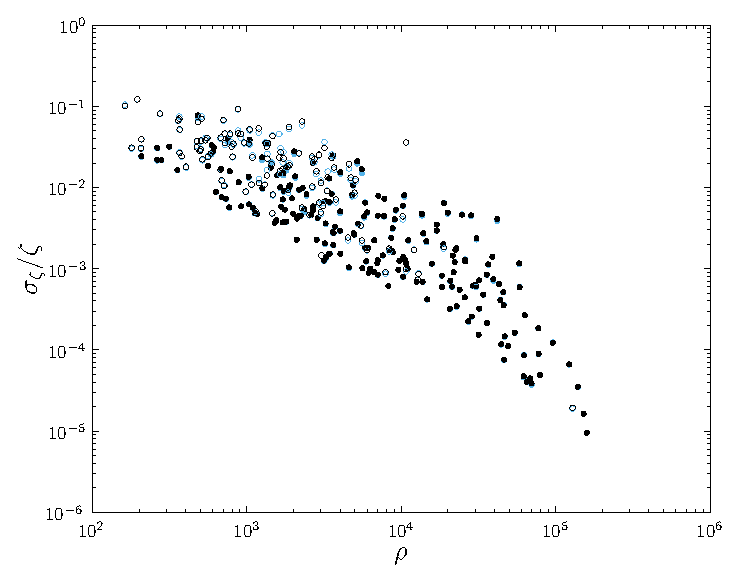
\includegraphics[width=0.485\textwidth]{./images/Fig_MW_MCMC_sigmas_SNR_10}} \\
\subfigure[Angular momentum $L_\infty$ versus periapsis.]{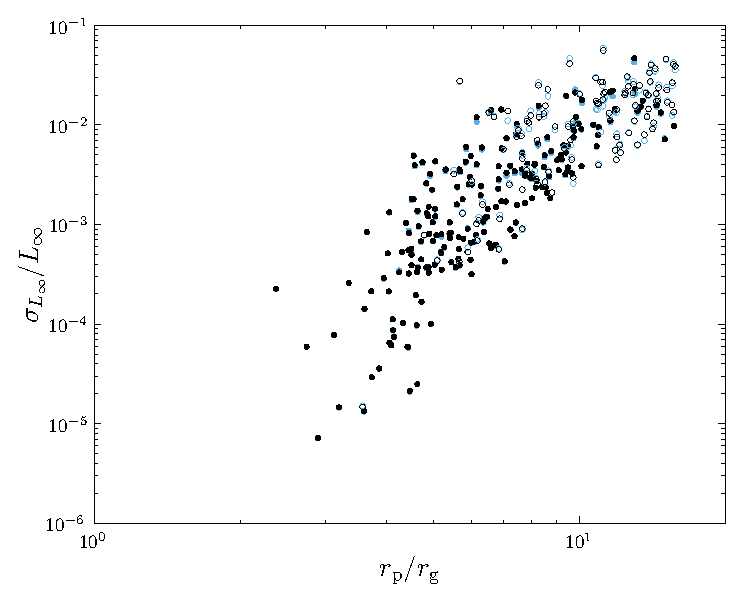
\includegraphics[width=0.475\textwidth]{./images/Fig_MW_MCMC_sigmas_rp_3}} \quad
\subfigure[Angular momentum $L_\infty$ versus SNR.]{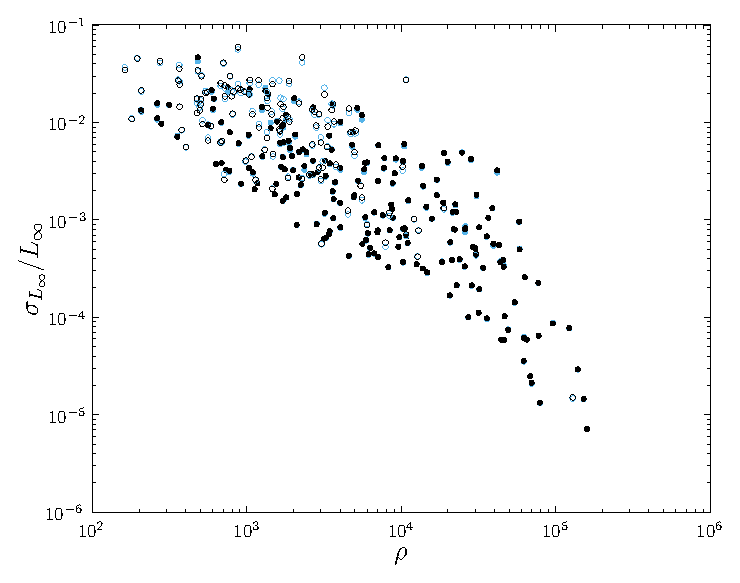
\includegraphics[width=0.485\textwidth]{./images/Fig_MW_MCMC_sigmas_SNR_3}} \\
\contcaption{{\bf{(Continued)}} Distribution widths as functions of periapse $r\sub{p}$ and SNR $\rho$.}
\end{figure}
\begin{figure}%[htp]
\setcounter{subfigure}{12}
\centering
\subfigure[Orbital inclination $\iota$ versus periapsis.]{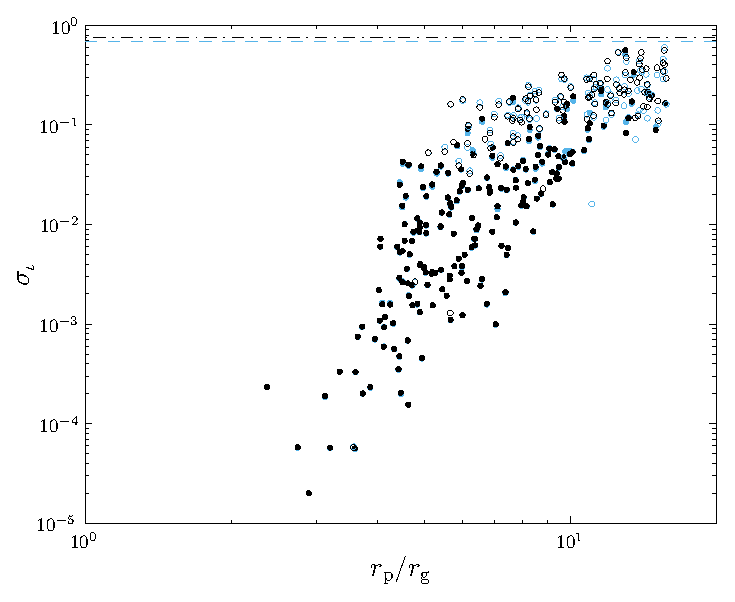
\includegraphics[width=0.475\textwidth]{./images/Fig_MW_MCMC_sigmas_rp_4}} \quad
\subfigure[Orbital inclination $\iota$ versus SNR.]{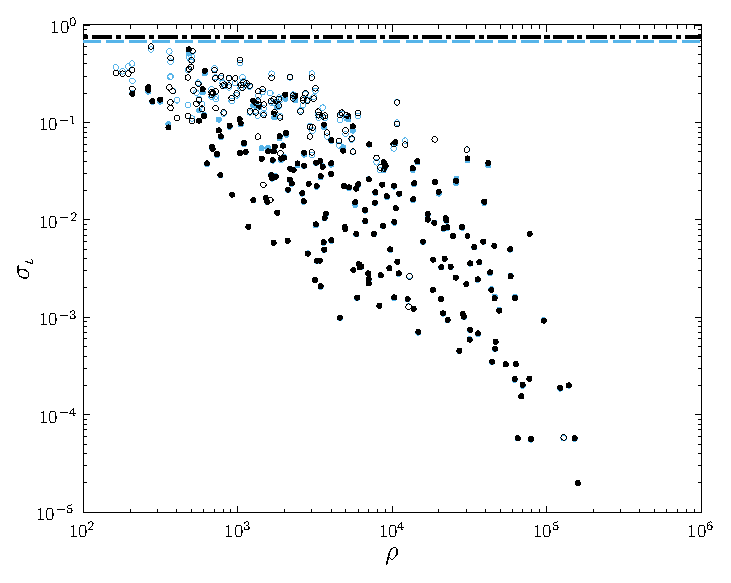
\includegraphics[width=0.485\textwidth]{./images/Fig_MW_MCMC_sigmas_SNR_4}} \\
\subfigure[Periapse azimuthal phase $\phi\sub{p}$ versus periapsis.]{\includegraphics[width=0.475\textwidth]{./images/Fig_MW_MCMC_sigmas_rp_7}} \quad
\subfigure[Periapse azimuthal phase $\phi\sub{p}$ versus SNR.]{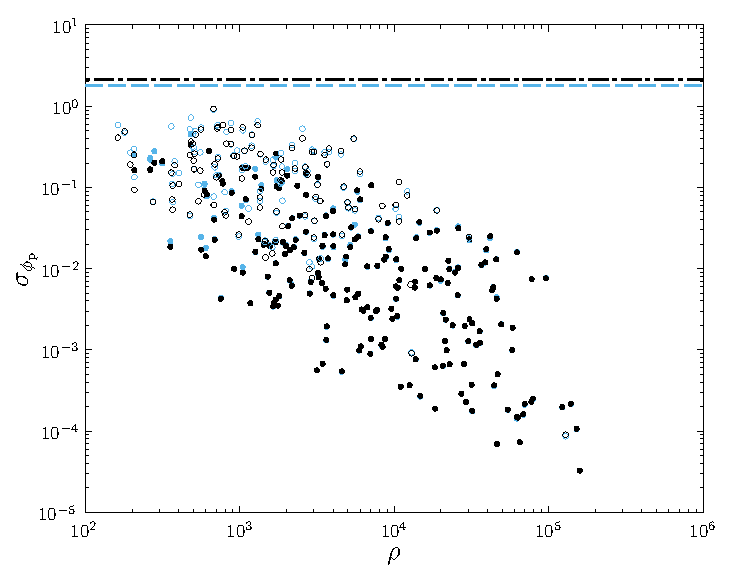
\includegraphics[width=0.485\textwidth]{./images/Fig_MW_MCMC_sigmas_SNR_7}} \\
\subfigure[Periapse polar phase $\chi\sub{p}$ versus periapsis.]{\includegraphics[width=0.475\textwidth]{./images/Fig_MW_MCMC_sigmas_rp_5}} \quad
\subfigure[Periapse polar phase $\chi\sub{p}$ versus SNR.]{\includegraphics[width=0.485\textwidth]{./images/Fig_MW_MCMC_sigmas_SNR_5}} \\
\contcaption{{\bf{(Continued)}} Distribution widths as functions of periapse $r\sub{p}$ and SNR $\rho$.}
\end{figure}
\begin{figure}%[t]
\setcounter{subfigure}{18}
\centering
\subfigure[Periapse time $t\sub{p}$ versus periapsis.]{\includegraphics[width=0.475\textwidth]{./images/Fig_MW_MCMC_sigmas_rp_6}} \quad
\subfigure[Periapse time $t\sub{p}$ versus SNR.]{\includegraphics[width=0.485\textwidth]{./images/Fig_MW_MCMC_sigmas_SNR_6}} \\
\contcaption{{\bf{(Concluded)}} Distribution widths as functions of periapsis $r\sub{p}$ and SNR $\rho$.}
\setcounter{subfigure}{0}
\end{figure}
For guidance, the dotted line corresponds to the current measurement uncertainty for $M_\bullet$; the dashed lines are $\sigma\sub{SD}$ from uniform priors for $a_\ast$, $\Phi\sub{K}$, $\phi\sub{p}$, $\chi\sub{p}$, $\cos\Theta\sub{K}$ and $\cos\iota$, and the dot--dashed lines are the equivalent $\sigma_{0.68}$. We have no expectations for the width of the MBH mass distribution with respect to the current value. However, we would expect that the recovered distributions for the other parameters are narrower than for the case of complete ignorance; this bound does seem to be respected. The two widths, $\sigma\sub{SD}$ and $\sigma_{0.68}$, typically agree better at smaller periapses and higher SNRs, as would be expected for more Gaussian distributions.

The widths show a trend of decreasing with decreasing periapsis or increasing SNR, but there is a large degree of scatter. There does not appear to be a strong dependence upon any single input parameter, with the exception of the spin. The widths for $\iota$, $\Theta\sub{K}$, $\Phi\sub{K}$, $\phi\sub{p}$ and $\chi\sub{p}$ increase for smaller spin magnitudes. The dependence is shown in \figref{sigmas-spin}.
\begin{figure}%[htp]
\centering
\subfigure[MBH spin $a_\ast$.]{\includegraphics[width=0.48\textwidth]{./images/Fig_MCMC_sigmas_rp_spin_2}} \quad
\subfigure[Orientation angle $\Theta\sub{K}$.]{\includegraphics[width=0.48\textwidth]{./images/Fig_MCMC_sigmas_rp_spin_8}} \\
\subfigure[Orientation angle $\Phi\sub{K}$.]{\includegraphics[width=0.48\textwidth]{./images/Fig_MCMC_sigmas_rp_spin_9}} \quad
\subfigure[Orbital inclination $\iota$.]{\includegraphics[width=0.48\textwidth]{./images/Fig_MCMC_sigmas_rp_spin_4}} \\
\subfigure[Periapse azimuthal phase $\phi\sub{p}$]{\includegraphics[width=0.48\textwidth]{./images/Fig_MCMC_sigmas_rp_spin_7}} \quad
\subfigure[Periapse polar phase $\chi\sub{p}$.]{\includegraphics[width=0.48\textwidth]{./images/Fig_MCMC_sigmas_rp_spin_5}}
\caption{Parameter standard deviations versus periapsis $r\sub{p}$, showing dependence (or lack thereof) upon the spin magnitude $|a_\ast|$.}
\label{fig:sigmas-spin}
\end{figure}
These parameters are defined with reference to the coordinate system established by the spin axis: for $a_\ast = 0$ we have spherical symmetry and there would be ambiguity in defining them. Therefore, it makes sense that they can be more accurately determined for larger spin magnitudes. The width for $a_\ast$, however, shows no clear correlation.

Comparing our MCMC and FIM results, we see there can be significant differences. Most parameters give results consistent to within an order (or two) of magnitude. The best agreement is for $t\sub{p}$, which is largely uncorrelated with the other parameters. The widths for $M_\bullet$, $a_\ast$, $L_\infty$ and $\iota$ show more severe differences; these parameters show the tightest degeneracies. The two methods do show signs of slowly converging with increasing SNR, as expected.

As a consistency check, to verify that the mismatch between the FIM and MCMC results is a consequence of parameter correlations, we calculated one-dimensional FIMs, only varying the MBH mass, and compared these to widths computed from MCMCs only sampling in mass. These were found to be in good agreement. The majority ($\sim 87\%$) have standard deviations consistent to within a factor of two; the rest within an order of magnitude.\footnote{One differed by more than an order of magnitude, and also failed to fulfil the (one-dimensional) MM criterion; this was a numerical problem in calculating the FIM.} Some small difference is expected because of numerical error from calculating derivatives for the FIM by finite differencing.

\subsection{Scientific potential}

Having quantified the precision with which we could infer parameters from an EMRB waveform, we can now consider if it is possible to learn anything new.

Of paramount interest are the MBH mass and spin. The current uncertainty in the mass is $\sigma_{M_\bullet} = 0.36 \times 10^6 M_\odot$ ($\sim 8\%$; \citealt{Gillessen2009}). There are few runs amongst our data set that are not better than this: it appears that orbits of a $\mu = 10 M_\odot$ CO with periapses $r\sub{p} \lesssim 13 r\sub{g}$ should be able to match our current observational constraints. However, the EMRB is an independent measurement, and so a measurement of comparable precision to the current bound can still be informative. Accuracy of $1\%$ could be possible if $r\sub{p} \lesssim 8 r\sub{g}$.

The spin is less well constrained. To obtain an uncertainty for the magnitude of $0.1$, comparable to that achieved in X-ray measurements of AGN, it appears that the periapsis needs to be $r\sub{p} \lesssim 11 r\sub{g}$. For smaller periapses, the uncertainty can be much less, indicating that an EMRB could be an excellent probe. The orientation angles for the spin axis may be constrained to better than $0.1$ for $r\sub{p} \lesssim 11 r\sub{g}$. It may well be possible to learn both the direction and the magnitude of the spin. This could illuminate the MBH's formation.

We have no {\it a priori} knowledge about the CO or its orbit, so anything we learn would be new. However, this is not particularly useful information, unless we observe multiple bursts, and can start to build up statistics for the dynamics of the GC. Using current observations for the distance to the GC, which could be further improved by the mass measurement from the EMRB, it is possible to infer a value for the mass $\mu$ from $\zeta$. This could inform us of the nature of the object (BH, NS or WD) and be a useful consistency check. A small value of $\zeta$, indicating a massive CO, is unambiguous evidence for the existence of a stellar-mass BH.

\section{Summary and conclusions}

We have analysed the properties of EMRBs from the GC. We used NK waveforms built using spherical polar and oblate-spheroidal coordinates. The two coordinate schemes yield almost indistinguishable results. There may be differences when the spin is large and the periapse is small: $\sim 10\%$ for $r\sub{p} \simeq 4 r\sub{g}$, $\sim 20\%$ for $r\sub{p} \simeq 2 r\sub{g}$. This is less than the error inherent in the semirelativistic approximation as inferred from the difference in NK and BH perturbation theory energy fluxes in \secref{Energy}. We conclude that either coordinate choice is valid for this purpose, and have adopted spherical polar coordinates.

The SNR of bursts is well correlated with the periapsis, it can be reasonably described as having a power law dependence. Using LISA, signals should be detectable for a $1 M_\odot$ ($10 M_\odot$) object if the periapse is $r\sub{p} < 27 r\sub{g}$ ($r\sub{p} < 65 r\sub{g}$), corresponding to a physical scale of $1.7 \times 10^{11}\units{m}$ ($4.1 \times 10^{11}\units{m}$) or $5.6 \times 10^{-6}\units{pc}$ ($1.3 \times 10^{-5}\units{pc}$). Using eLISA, these distances are approximately three times smaller.

We conducted an investigation using Fisher matrix analysis into how precisely we could infer parameters of the GC's MBH. However, we found that the LSA does not hold for these bursts over a wide range of SNR. This demonstrates the necessity of checking the approximation before quoting the results of an FIM analysis \citep{Vallisneri2008}.

We used MCMC results as a more robust measure of parameter estimation accuracy. Potentially, it is possible to determine very precisely the key parameters defining the MBH's mass and spin, if the orbit gets close enough to the MBH. It appears that we can achieve good results from a single EMRB with periapsis of $r\sub{p} \simeq 10 r\sub{g}$ for a $10 M_\odot$ CO. This translates to a distance of $6 \times 10^{10}\units{m}$ or $2 \times 10^{-6}\units{pc}$. Orbits closer than this would place stricter constraints. The best orbits yield uncertainties of almost one part in $10^5$ for the MBH mass and spin, far exceeding existing techniques. Conversely, orbits with $r\sub{p} \gtrsim 16 r\sub{g}$ are unlikely to provide any useful information.

Before we can quote results for how accurately we can determine the various parameters, we must consider the probability of each orbit. This shall be done in \chapref{events}.

We have so far only considered EMRBs from our Galaxy; a natural extension is to consider bursts from extragalactic sources, which we do in the next chapter. Extragalactic bursts are not as promising as those from the GC, but could still make a significant contribution to the total burst event rate. 


\part{Understanding gravitation}

\chapter{Gravitational radiation in $f(R)$-gravity}\label{ch:f-R1}

\section{Beyond general relativity: $f(R)$ modified gravity}

GR is a well tested theory of gravity \citep{Will2006}; however, the majority of the tests that have been carried out to date have been in the weak-field, low-energy regime \citep{Will1993,Psaltis2008a}. It is not unreasonable to suspect there may be higher order corrections that are only discovered in the strong-field regime, where curvature is high or spacetime dynamic.

In this and the following chapter, we shall study a modified theory of gravitation to assess the feasibility of potential corrections to GR. We investigate metric $f(R)$-gravity, in which the Einstein--Hilbert action is modified by replacing the Ricci scalar $R$ with an arbitrary function $f(R)$. This is one of the simplest extensions to standard GR \citep{Sotiriou2010, DeFelice2010}. It has attracted significant interest because the flexibility in defining the function $f(R)$ allows a wide range of cosmological phenomena to be described \citep{Nojiri2007, Capozziello2007a}. For example, \citet{Starobinsky1980} suggested that a quadratic addition to the field equations could drive exponential expansion of the early Universe \citep{Vilenkin1985}: inflation in modern terminology. In this model $f(R) = R - R^2/(6\Upsilon^2)$; the size of the quadratic correction can be tightly constrained by considering the spectrum of curvature perturbations generated during inflation \citep{Starobinskii1983, Starobinskii1985}. Using the results of the Wilkinson Microwave Anisotropy Probe (WMAP; \citealt{Bennett2012, Hinshaw2012}) and Planck \citep{Ade2013a,Ade2013b}, the inverse length-scale can be constrained to $\Upsilon \simeq 3.0 \times 10^{-6} \ell\sub{P}^{-1}$, where $\ell\sub{P}$ is the Planck length and the number of $e$-folds during inflation is assumed to be $N = 2/(1 - n_s)$, for scalar spectrum power-law index $n_s$ \citep{Starobinsky2007, DeFelice2010}. % $\Upsilon \simeq 2.9 \times 10^{-6} (50/N) \ell\sub{P}^{-1}$. % Upsilon = sqrt(3 pi P)/N l_p; N = 2 / (1 - n_s); WMAP P = Delta_R^2 = 2.464e-9, n_s = 0.9608; Planck P = A_s = 2.196e-9; n_s = 0.9603.

We consider simple $f(R)$ corrections within the framework of linearised gravity and discover how GWs are modified. We begin by reviewing the properties of the $f(R)$ field equations. We then derive the linearised equations (\secref{Lin}) and use these to determine the properties of GWs (\secref{Rad}). These are largely known in the literature, but are worked out here {\it ab initio}. We proceed to derive an effective energy-momentum tensor for gravitational radiation in \secref{EM_tensor}, following the short-wavelength approximation of \citet{Isaacson1968, Isaacson1968a}.

Following on from the theory developed in this chapter, in \chapref{f-R2} we consider observational tests of $f(R)$-gravity. We explore what constraints LISA, Solar System tests and laboratory experiments can place on the form of $f(R)$. We do not consider cosmological implications where terms beyond linear order could play a significant role. The overall conclusion is that LISA could place constraints on $f(R)$-gravity which may be more powerful than those in the Solar System, but are not as powerful as constraints from laboratory experiments. A brief summary of findings from both chapters is found in \secref{f_Discuss}.

Natural units with $c = 1$ are used throughout both chapters, but factors of $G$ are retained.

\section{Description of $f(R)$-gravity}

\subsection{The action and field equations}\label{sec:Action}

General relativity can be derived from the Einstein--Hilbert action (\citealt[chapter 21]{Misner1973}; \citealt[section 93]{Landau1975}; \citealt[section 26]{Dirac1996})
\begin{equation}
S\sub{EH}[g] = \recip{16\pi G}\intd{}{}{R\sqrt{-g}}{^4x}.
\end{equation}
In $f(R)$ theory we make a simple modification of the action to include an arbitrary function of the Ricci scalar $R$ such that \citep{Buchdahl1970}
\begin{equation}
S_{f(R)}[g] = \recip{16\pi G}\intd{}{}{f(R)\sqrt{-g}}{^4x}.
\end{equation}
Including the function $f(R)$ gives extra freedom in defining the behaviour of gravity. While this action may not encode the true theory of gravity it could contain sufficient information to act as an effective field theory, correctly describing phenomenological behaviour \citep{Park2010}; it may be that as an effective field theory, a particular $f(R)$ shall have a limited region of applicability and shall not be universal. We assume that $f(R)$ is analytic about $R = 0$ so that it can be expressed as a power series \citep{Buchdahl1970, Faulkner2007, Clifton2008} %\citep{Buchdahl1970, Capozziello2007, Faulkner2007, Clifton2008, Psaltis2008}
\begin{equation}
f(R) = a_0 + a_1 R + \dfrac{a_2}{2!}R^2 + \dfrac{a_3}{3!}R^3 + \ldots
\end{equation}
Since the dimensions of $f(R)$ must be the same as of $R$, $[a_n] = [R]^{(1-n)}$. To link to GR we set $a_1 = 1$; any rescaling can be absorbed into the definition of $G$.

Various models of cosmological interest may be expressed in such a form, for example, the model of \citet{Starobinsky2007}
\begin{equation}
f(R) = R + \lambda R_0 \left[\left(1 + \dfrac{R^2}{R_0^2}\right)^{-n} - 1\right],
\end{equation}
can be expanded as
\begin{equation}
f(R) = R - \dfrac{\lambda n}{R_0} R^2 + \dfrac{\lambda n (n + 1)}{2 R_0^3} R^4 + \ldots
\end{equation}
and the model of \citet{Hu2007}
\begin{equation}
f(R) = R - m^2\dfrac{c_1\left(R/m^2\right)^n}{c_2\left(R/m^2\right)^n + 1},
\end{equation}
assuming that $c_2(R/m^2)^n \ll 1$, can be expanded as
\begin{equation}
f(R) = (1 - c_1)R + \dfrac{c_1 c_2}{m^2}R^2 - \dfrac{c_1 c_2^2}{m^4}R^3 + \dfrac{c_1 c_2^3}{m^6}R^4 + \ldots 
\end{equation}
for $n = 1$ and as
\begin{equation}
f(R) = R - \dfrac{c_1}{m^2}R^2 + \dfrac{c_1 c_2^2}{m^4}R^4 + \ldots
\end{equation}
for $n = 2$. Consequently such a series expansion can constrain model parameters, although we cannot specify the full functional form from only a few terms.

The field equations are obtained by a variational principle; there are several ways of achieving this. To derive the Einstein field equations from the Einstein--Hilbert action one may use the standard metric variation or the Palatini variation \citep[section 21.2]{Misner1973}. Both approaches can be used for $f(R)$, but they yield different results \citep{Sotiriou2010, DeFelice2010}. Following the metric formalism, one varies the action with respect to the metric $g^{\mu\nu}$. Following the Palatini formalism one varies the action with respect to both the metric $g^{\mu\nu}$ and the connection ${\Gamma^\rho}_{\mu\nu}$, which are treated as independent quantities: the connection is not the Levi-Civita metric connection.\footnote{Imposing the condition that the metric and Palatini formalisms produce the same field equations, assuming an action that only depends on the metric and Riemann tensor, results in Lovelock gravity \citep{Exirifard2008}. Lovelock gravities require the field equations to be divergence free and no more than second order; in four dimensions the only possible Lovelock gravity is GR with a potentially non-zero cosmological constant \citep{Lovelock1970, Lovelock1971, Lovelock1972}.}

Finally, there is a third version of $f(R)$-gravity: metric-affine $f(R)$-gravity \citep{Sotiriou2007, Sotiriou2007b}. This goes beyond the Palatini formalism by supposing that the matter action is dependent on the variational independent connection. Parallel transport and the covariant derivative are divorced from the metric. This theory has its attractions: it allows for a natural introduction of torsion. However, it is not a metric theory of gravity and so cannot satisfy all the postulates of the Einstein equivalence principle \citep{Will2006}: a free particle does not necessarily follow a geodesic and so the effects of gravity might not be locally removed \citep{Exirifard2008}. The implications of this have not been fully explored, but for this reason we will not consider the theory further.

We restrict our attention to metric $f(R)$-gravity. This is preferred as the Palatini formalism has undesirable properties: static spherically symmetric objects described by a polytropic equation of state are subject to a curvature singularity \citep{Barausse2008b, Barausse2008a, DeFelice2010}. Varying the action with respect to the metric $g^{\mu\nu}$ produces
\begin{align}
\delta S_{f(R)} = {} & \recip{16\pi G}\int\left\{f'(R)\sqrt{-g}\left[R_{\mu\nu} - \nabla_\mu\nabla_\nu\ + g_{\mu\nu}\Box\right] \hphantom{\dfrac{0}{0}} \vphantom{\dfrac{0}{0}} - f(R)\recip{2}\sqrt{-g}g_{\mu\nu}\right\}\delta g^{\mu\nu}\,\dd^4x,
\end{align}
where $\Box = g^{\mu\nu}\nabla_\mu\nabla_\nu$ is the d'Alembertian and a prime denotes differentiation with respect to $R$.

Proceeding from here requires certain assumptions regarding surface terms. In the case of the Einstein--Hilbert action these gather into a total derivative; it is possible to subtract this from the action to obtain a well-defined variational quantity \citep{York1972Jr, Gibbons1977}. This is not the case for general $f(R)$-gravity \citep{Madsen1989}. However, since the action includes higher-order derivatives of the metric, we are at liberty to fix more degrees of freedom at the boundary, in so doing eliminating the importance of the surface terms \citep{Dyer2009a, Sotiriou2010}. Setting the variation $\delta R = 0$ on the boundary allows us to subtract a term similar to that in GR \citep{Guarnizo2010}. We then have a well-defined variational quantity, from which we can obtain the field equations.

The vacuum field equations are
\begin{equation}
f'R_{\mu\nu} - \nabla_\mu\nabla_\nu f' + g_{\mu\nu}\Box f' - \dfrac{f}{2}g_{\mu\nu} = 0.
\label{eq:Field_eq}
\end{equation}
Taking the trace gives
\begin{equation}
f'R + 3\Box f' - 2f = 0.
\label{eq:Trace_eq}
\end{equation}
If we consider a uniform flat spacetime $R = 0$, this requires \citep{Capozziello2007}
\begin{equation}
a_0 = 0.
\label{eq:a_0}
\end{equation}
In analogy to the Einstein tensor, we define
\begin{equation}
\mathcal{G}_{\mu\nu} = f'R_{\mu\nu} - \nabla_\mu\nabla_\nu f' + g_{\mu\nu}\Box f' - \dfrac{f}{2}g_{\mu\nu},
\label{eq:G_tensor}
\end{equation}
so that in a vacuum
\begin{equation}
\mathcal{G}_{\mu\nu} = 0.
\end{equation}

\subsection{Conservation of energy-momentum}

If we introduce matter with a stress-energy tensor $T_{\mu\nu}$, the field equations become
\begin{equation}
\mathcal{G}_{\mu\nu} = 8\pi GT_{\mu\nu}.
\end{equation}
Acting upon this with the covariant derivative
\begin{align}
8\pi G\nabla^\mu T_{\mu\nu} = {} & \nabla^\mu\mathcal{G}_{\mu\nu} \nonumber \\*
 = {} & R_{\mu\nu}\nabla^\mu f' + f'\nabla^\mu\left(R_{\mu\nu} - \recip{2}R g_{\mu\nu}\right) - \left(\Box\nabla_\nu - \nabla_\nu\Box\right)f'.
\end{align}
The second term contains the covariant derivative of the Einstein tensor and so is zero. The final term can be shown to be
\begin{equation}
\left(\Box\nabla_\nu - \nabla_\nu\Box\right)f' = R_{\mu\nu}\nabla^\mu f',
\end{equation}
which is a useful geometric identity \citep{Koivisto2006a}. Using this
\begin{equation}
8\pi G\nabla^\mu T_{\mu\nu} = 0.
\end{equation}
Consequently energy-momentum is a conserved quantity in the same way as in GR, as is expected from the symmetries of the action.

\section{Linearised theory}\label{sec:Lin}

We start our investigation of $f(R)$ by looking at linearised theory. This is a weak-field approximation that assumes only small deviations from a flat background, greatly simplifying the field equations. Just as in GR, the linearised framework provides a natural way to study GWs. We shall see that the linearised field equations reduce down to flat-space wave equations: GWs are as much a part of $f(R)$-gravity as of GR.

Consider a perturbation of the metric from flat Minkowski space such that
\begin{equation}
g_{\mu\nu} = \eta_{\mu\nu} + h_{\mu\nu};
\end{equation}
where, more formally, $h_{\mu\nu} = \varepsilon H_{\mu\nu}$ for a small parameter $\varepsilon$.\footnote{It is because we wish to perturb about flat spacetime that we have required $f(R)$ to be analytic about $R = 0$.} We only consider terms to $\order{\varepsilon}$. The inverse metric is then
\begin{equation}
g^{\mu\nu} = \eta^{\mu\nu} - h^{\mu\nu},
\end{equation}
where we have used the Minkowski metric to raise the indices on the right, defining
\begin{equation}
h^{\mu\nu} = \eta^{\mu\sigma}\eta^{\nu\rho}h_{\sigma\rho}.
\end{equation}
Similarly, the trace $h$ is given by
\begin{equation}
h = \eta^{\mu\nu}h_{\mu\nu}.
\end{equation}
All quantities denoted by ``$h$'' are strictly $\order{\varepsilon}$.

The linearised connection is
\begin{equation}
{{\Gamma^{(1)}}^\rho}_{\mu\nu} = \dfrac{1}{2}\eta^{\rho\lambda}(\partial_\mu h_{\lambda\nu} + \partial_\nu h_{\lambda\mu} - \partial_\lambda h_{\mu\nu}).
\label{eq:Lin_Gamma}
\end{equation}
To $\order{\varepsilon}$ the covariant derivative of any perturbed quantity is the same as the partial derivative. The Riemann tensor is
\begin{equation}
{{R^{(1)}}^\lambda}_{\mu\nu\rho} = \dfrac{1}{2}(\partial_\mu\partial_\nu h^\lambda_\rho + \partial^\lambda\partial_\rho h_{\mu\nu} - \partial_\mu\partial_\rho h^\lambda_\nu - \partial^\lambda\partial_\nu h_{\mu\rho}),
\label{eq:Lin_Riemann}
\end{equation}
where we have raised the index on the differential operator with the background Minkowski metric. Contracting gives the Ricci tensor
\begin{equation}
{R^{(1)}}_{\mu\nu} = \dfrac{1}{2}(\partial_\mu\partial_\rho h^\rho_\nu + \partial_\nu\partial_\rho h^\rho_\mu - \partial_\mu\partial_\nu h - \Box h_{\mu\nu}),
\label{eq:Ricci}
\end{equation}
where the d'Alembertian operator is $\Box = \eta^{\mu\nu}\partial_\mu\partial_\nu$. Contracting this with $\eta^{\mu\nu}$ gives the first-order Ricci scalar
\begin{equation}
R^{(1)} = \partial_\mu\partial_\rho h^{\rho\mu} - \Box h.
\label{eq:Scalar}
\end{equation}

To $\order{\varepsilon}$ we can write $f(R)$ as a Maclaurin series
\begin{subequations}
\begin{align}
f(R) = {} & a_0 + R^{(1)}; \\
f'(R) = {} & 1 + a_2 R^{(1)}.
\end{align}
\end{subequations}
As we are perturbing from a Minkowski background where the Ricci scalar vanishes, we use \eqnref{a_0} to set $a_0 = 0$. Inserting these into \eqnref{G_tensor} and retaining terms to $\order{\varepsilon}$ yields
\begin{equation}
{\mathcal{G}^{(1)}}_{\mu\nu} = {R^{(1)}}_{\mu\nu} - \partial_\mu\partial_\nu(a_2 R^{(1)}) + \eta_{\mu\nu}\Box(a_2 R^{(1)}) - \dfrac{R^{(1)}}{2}\eta_{\mu\nu}.
\label{eq:Field}
\end{equation}
Now consider the linearised trace equation, from \eqnref{Trace_eq}
\begin{align}
\mathcal{G}^{(1)} = {} & R^{(1)} + 3 \Box(a_2 R^{(1)}) - 2 R^{(1)} \nonumber \\*
 = {} & 3 \Box(a_2 R^{(1)}) - R^{(1)},
\label{eq:Box_R}
\end{align}
where $\mathcal{G}^{(1)} = \eta^{\mu\nu}{\mathcal{G}^{(1)}}_{\mu\nu}$. This is the massive inhomogeneous Klein-Gordon equation. Setting $\mathcal{G} = 0$, as for a vacuum, we obtain the standard Klein-Gordon equation
\begin{equation}
\Box R^{(1)} + \Upsilon^2 R^{(1)} = 0,
\end{equation}
defining the reciprocal length (squared)
\begin{equation}
\Upsilon^2 = -\recip{3a_2}.
\end{equation}
For a physically meaningful solution $\Upsilon^2 > 0$: we constrain $f(R)$ such that $a_2 < 0$ \citep{Schmidt1986, Teyssandier1990, Olmo2005c, Corda2008}. From $\Upsilon$ we define a reduced Compton wavelength
\begin{equation}
\lambdabar_R = \recip{\Upsilon}
\end{equation}
associated with this scalar mode.

The next step is to substitute in $h_{\mu\nu}$ to find wave solutions. We want a quantity $\overline{h}_{\mu\nu}$ that satisfies a wave equation, related to $h_{\mu\nu}$ by
\begin{equation}
\overline{h}_{\mu\nu} = h_{\mu\nu} + A_{\mu\nu}.
\end{equation}
In GR we use the trace-reversed form where $A_{\mu\nu} = -(h/2)\eta_{\mu\nu}$. This does not suffice here, but let us look for a similar solution
\begin{equation}
\overline{h}_{\mu\nu} = h_{\mu\nu} - \dfrac{h}{2}\eta_{\mu\nu} + B_{\mu\nu}.
\end{equation}
The only rank-two tensors in our theory are: $h_{\mu\nu}$, $\eta_{\mu\nu}$, ${R^{(1)}}_{\mu\nu}$, and $\partial_\mu\partial_\nu$; $h_{\mu\nu}$ has been used already, and we wish to eliminate ${R^{(1)}}_{\mu\nu}$, so we can try the simpler option based around $\eta_{\mu\nu}$. We want $B_{\mu\nu}$ to be $\order{\varepsilon}$; since we have already used $h$, we shall try the other scalar quantity $R^{(1)}$. Therefore, we construct an ansatz
\begin{equation}
\overline{h}_{\mu\nu} = h_{\mu\nu} + \left(b a_2 R^{(1)} - \dfrac{h}{2}\right)\eta_{\mu\nu},
\label{eq:Ansatz}
\end{equation}
where $a_2$ has been included to ensure dimensional consistency and $b$ is a dimensionless number. Contracting with the background metric yields
\begin{equation}
\overline{h} = 4b a_2 R^{(1)} - h,
\label{eq:h_trace}
\end{equation}
so we can eliminate $h$ in our definition of $\overline{h}_{\mu\nu}$ to give
\begin{equation}
h_{\mu\nu} = \overline{h}_{\mu\nu} + \left(b a_2 R^{(1)} -\dfrac{\overline{h}}{2}\right)\eta_{\mu\nu}.
\end{equation}
Just as in GR, we have the freedom to perform a gauge transformation (\citealt[box 18.2]{Misner1973}; \citealt[section 17.1]{Hobson2006}): the field equations are gauge-invariant since we started with a function of the gauge-invariant Ricci scalar. We shall assume a Lorenz, or de Donder, gauge choice
\begin{equation}
\nabla^\mu \overline{h}_{\mu\nu} = 0;
\end{equation}
or for a flat spacetime
\begin{equation}
\partial^\mu \overline{h}_{\mu\nu} = 0.
\label{eq:Lorenz}
\end{equation}
Subject to this, from \eqnref{Ricci}, the Ricci tensor is
\begin{align}
{R^{(1)}}_{\mu\nu} = {} & -\left[b \partial_\mu\partial_\nu(a_2  R^{(1)}) + \recip{2}\Box\left(\overline{h}_{\mu\nu} -\dfrac{\overline{h}}{2}\eta_{\mu\nu}\right) + \dfrac{b}{6}(R^{(1)} + \mathcal{G}^{(1)})\eta_{\mu\nu}\right].
\label{eq:new_Ricci}
\end{align}
Using this with \eqnref{Box_R} in \eqnref{Field} gives
\begin{align}
{\mathcal{G}^{(1)}}_{\mu\nu} = {} & \dfrac{2 - b}{6}\mathcal{G}^{(1)}\eta_{\mu\nu} -\dfrac{1}{2}\Box\left(\overline{h}_{\mu\nu} - \dfrac{\overline{h}}{2}\eta_{\mu\nu}\right) - (b + 1)\left[\partial_\mu\partial_\nu(a_2 R^{(1)}) + \recip{6}R^{(1)}\eta_{\mu\nu}\right].
\label{eq:b_Field}
\end{align}
Picking $b = -1$ the final term vanishes, thus we set (\citealt[section 10.3]{Will1993}; \citealt{Corda2008, Capozziello2008}) % Will section 10.3
\begin{subequations}
\begin{align}
\label{eq:hbar_metric}
\overline{h}_{\mu\nu} = {} & h_{\mu\nu} - \left(a_2 R^{(1)} + \dfrac{h}{2}\right)\eta_{\mu\nu}\\
h_{\mu\nu} = {} & \overline{h}_{\mu\nu} - \left(a_2 R^{(1)} + \dfrac{\overline{h}}{2}\right)\eta_{\mu\nu}.
\label{eq:h_metric}
\end{align}
\end{subequations}
From \eqnref{Scalar} the Ricci scalar is 
\begin{align}
R^{(1)} = {} & \Box \left(a_2 R^{(1)} -\dfrac{\overline{h}}{2}\right) + \Box (4 a_2 R^{(1)} + \overline{h}) \nonumber \\*
 = {} & 3 \Box(a_2 R^{(1)}) + \dfrac{1}{2}\Box \overline{h}.
\label{eq:Ricci_Box_h}
\end{align}
For consistency with \eqnref{Box_R}, we require
\begin{equation}
-\recip{2}\Box \overline{h} = \mathcal{G}^{(1)}.
\label{eq:Box_h}
\end{equation}
Inserting this into \eqnref{b_Field}, with $b = -1$, we see
\begin{equation}
-\recip{2}\Box \overline{h}_{\mu\nu} = {\mathcal{G}^{(1)}}_{\mu\nu};
\label{eq:Box_hmunu}
\end{equation}
we have our wave equations.

Should $a_2$ be sufficiently small that it can be regarded an $\order{\varepsilon}$ quantity, we recover the usual GR formulae to leading order within our analysis.

\section{Gravitational radiation}\label{sec:Rad}

Having established two wave equations, \eqref{eq:Box_R} and \eqref{eq:Box_hmunu}, we now investigate their solutions. Consider waves in a vacuum, such that $\mathcal{G}_{\mu\nu} = 0$. Using a standard Fourier decomposition
\begin{subequations}
\begin{align}
\overline{h}_{\mu\nu} = {} & \widehat{h}_{\mu\nu}(k_\rho) \exp\left(ik_\rho x^\rho\right),\\
R^{(1)} = {} & \widehat{R}(q_\rho) \exp\left(iq_\rho x^\rho\right),
\end{align}
\end{subequations}
where $k_\mu$ and $q_\mu$ are four-wavevectors. From \eqnref{Box_hmunu} we know that $k_\mu$ is a null vector, so for a wave travelling along the $z$-axis
\begin{equation}
k^\mu = \omega(1, 0, 0, 1),
\end{equation}
where $\omega$ is the angular frequency. Similarly, from \eqnref{Box_R}
\begin{equation}
q^\mu = \left(\Omega, 0, 0, \sqrt{\Omega^2 - \Upsilon^2}\right),
\label{eq:Ricci_q}
\end{equation}
for frequency $\Omega$. These waves do not travel at $c$, but have a group velocity
\begin{equation}
v(\Omega) = \dfrac{\sqrt{\Omega^2 - \Upsilon^2}}{\Omega},
\end{equation}
provided that $\Upsilon^2 > 0$, $v < 1 = c$. For $\Omega < \Upsilon$, we find an evanescently decaying wave. The travelling wave is dispersive; for waves made up of a range of frequency components there shall be a time delay between the arrival of the high-frequency and low-frequency constituents. This may make it difficult to reconstruct a waveform, should the scalar mode be observed with a GW detector.

From the gauge condition \eqnref{Lorenz} we find that $k^\mu$ is orthogonal to $\widehat{h}_{\mu\nu}$,
\begin{equation}
k^\mu\widehat{h}_{\mu\nu} = 0,
\end{equation}
in this case
\begin{equation}
\widehat{h}_{0\nu} + \widehat{h}_{3\nu} = 0.
\label{eq:Transverse}
\end{equation}

Let us consider the implications of \eqnref{Box_h} using \eqref{eq:Box_R} and \eqref{eq:h_trace},
\begin{align}
\Box\left(4a_2R^{(1)} + h\right) = {} & 0 \nonumber \\*
\Box h = {} & -\dfrac{4}{3}R^{(1)}.
\end{align}
For non-zero $R^{(1)}$ (as required for the Ricci mode) there is no way to make a gauge choice such that the trace $h$ vanishes \citep{Corda2008, Capozziello2008}. This is distinct from in GR. It is possible, however, to make a gauge choice such that the trace $\overline{h}$ vanishes. Consider a gauge transformation generated by $\xi_\mu$ which satisfies $\Box \xi_\mu = 0$, and so has a Fourier decomposition
\begin{equation}
\xi_\mu = \widehat{\xi}_\mu \exp\left(ik_\rho x^\rho\right).
\end{equation}
A transformation
\begin{equation}
\overline{h}_{\mu\nu} \rightarrow \overline{h}_{\mu\nu} + \partial_\mu\xi_\nu + \partial_\nu\xi_\mu - \eta_{\mu\nu}\partial^\rho\xi_\rho,
\end{equation}
would ensure both conditions \eqref{eq:Lorenz} and \eqref{eq:Box_hmunu} are satisfied \cite[section 35.2]{Misner1973}. Under such a transformation
\begin{equation}
\widehat{h}_{\mu\nu} \rightarrow \widehat{h}_{\mu\nu} + i\left(k_\mu\widehat{\xi}_\nu + k_\nu\widehat{\xi}_\mu - \eta_{\mu\nu}k^\rho\widehat{\xi}_\rho\right).
\end{equation}
We may impose four further constraints (one for each $\widehat{\xi}_\mu$) upon $\widehat{h}_{\mu\nu}$. We take these to be \citep[section 4.4]{Wald1984}
\begin{equation}
\widehat{h}_{0\nu} = 0, \qquad \widehat{h} = 0.
\end{equation}
This might appear to be five constraints, but we have already imposed \eqnref{Transverse}, and so setting $\widehat{h}_{00} = 0$ automatically implies $\widehat{h}_{03} = 0$. In this gauge
\begin{equation}
h_{\mu\nu} = {} \overline{h}_{\mu\nu} - a_2 R^{(1)}\eta_{\mu\nu}; \quad h = {} -4a_2R^{(1)}.
\label{eq:gauge}
\end{equation}
Thus $\overline{h}_{\mu\nu}$ behaves just as its GR counterpart; we can define
\begin{equation}
\left[\widehat{h}_{\mu\nu}\right] =
\begin{bmatrix}
0 & 0 & 0 & 0\\
0 & h_+ & h_\times & 0\\
0 & h_\times & -h_+ & 0\\
0 & 0 & 0 & 0
\end{bmatrix},
\end{equation}
where $h_+$ and $h_\times$ are constants representing the amplitudes of the two transverse polarizations of gravitational radiation.

It is important that our solutions reduce to those of GR if $f(R) = R$. In our linearised approach this corresponds to $a_2 \rightarrow 0$, $\Upsilon^2 \rightarrow \infty$. We see from \eqnref{Ricci_q} that in this limit it would take an infinite frequency to excite a propagating Ricci mode, and evanescent waves would decay away infinitely fast. Therefore, there would be no detectable Ricci modes and we would only observe the two polarizations found in GR. Additionally, $\overline{h}_{\mu\nu}$ would simplify to its usual trace-reversed form.

\section{Energy-momentum tensor}\label{sec:EM_tensor}

We expect gravitational radiation to carry energy-momentum. Unfortunately, it is difficult to define a proper energy-momentum tensor for a gravitational field: as a consequence of the equivalence principle it is possible to transform to a freely falling frame, eliminating the gravitational field and any associated energy density at a given point, although we can still define curvature in the neighbourhood of this point (\citealt[section 20.4]{Misner1973}; \citealt[section 17.11]{Hobson2006}). We do nothing revolutionary, but follow the approach of \citet{Isaacson1968, Isaacson1968a}. The full field equations \eqref{eq:Field_eq} have no energy-momentum tensor for the gravitational field on the right-hand side; however, by expanding beyond the linear terms we can find a suitable effective energy-momentum tensor for GWs. Expanding $\mathcal{G}_{\mu\nu}$ in orders of $h_{\mu\nu}$
\begin{equation}
\mathcal{G}_{\mu\nu} = {\mathcal{G}^{(\text{B})}}_{\mu\nu} + {\mathcal{G}^{(1)}}_{\mu\nu} + {\mathcal{G}^{(2)}}_{\mu\nu} + \ldots
\label{eq:G_exp}
\end{equation}
We use $(\text{B})$ for the background term instead of $(0)$ to avoid confusion regarding its order in $\varepsilon$. So far we have assumed that our background is flat; however, we can imagine that should the gravitational radiation carry energy-momentum then this would act as a source of curvature for the background \citep[section 4.4b]{Wald1984}. This is a second-order effect that may be encoded, to accuracy of $\order{\varepsilon^2}$, as \citep[section 15.4]{Rindler2006}
\begin{equation}
{\mathcal{G}^{(\text{B})}}_{\mu\nu} = -{\mathcal{G}^{(2)}}_{\mu\nu}.
\end{equation}
By shifting ${\mathcal{G}^{(2)}}_{\mu\nu}$ to the right-hand side we create an effective energy-momentum tensor. As in GR we average over several wavelengths, assuming that the background curvature is on a larger scale (\citealt[section 35.13]{Misner1973}; \citealt{Stein2011}),
\begin{equation}
{\mathcal{G}^{(\text{B})}}_{\mu\nu} = -\left\langle{\mathcal{G}^{(2)}}_{\mu\nu}\right\rangle.
\end{equation}
By averaging we probe the curvature in a macroscopic region about a given point in spacetime, yielding a gauge-invariant measure of the gravitational field strength. The averaging can be thought of as smoothing out the rapidly varying ripples of the radiation, leaving only the coarse-grained component that acts as a source for the background curvature.\footnote{By averaging we do not try to localise the energy of a wave to within a wavelength; for the massive Ricci scalar mode we always consider scales greater than $\lambda_R$.} The effective energy-momentum tensor for the radiation is
\begin{equation}
t_{\mu\nu} = -\recip{8\pi G}\left\langle{\mathcal{G}^{(\text{2})}}_{\mu\nu}\right\rangle.
\end{equation}

Having made this provisional identification, we must set about carefully evaluating the various terms in \eqnref{G_exp}. We begin as in \secref{Lin} by defining a total metric
\begin{equation}
g_{\mu\nu} = \gamma_{\mu\nu} + h_{\mu\nu},
\end{equation}
where $\gamma_{\mu\nu}$ is the background metric. This changes our definition for $h_{\mu\nu}$: instead of being the total perturbation from flat Minkowski, it is the dynamical part of the metric with which we associate radiative effects. Since we know that ${\mathcal{G}^{(\text{B})}}_{\mu\nu}$ is $\order{\varepsilon^2}$, we decompose our background metric as
\begin{equation}
\gamma_{\mu\nu} = \eta_{\mu\nu} + j_{\mu\nu},
\end{equation}
where $j_{\mu\nu}$ is $\order{\varepsilon^2}$ to ensure that ${{R^{(\text{B})}}^\lambda}_{\mu\nu\rho}$ is also $\order{\varepsilon^2}$. Therefore its introduction makes no difference to the linearised theory.

We consider terms only to $\order{\varepsilon^2}$. We identify ${{\Gamma^{(1)}}^\rho}_{\mu\nu}$ from \eqnref{Lin_Gamma}.\footnote{There is one small subtlety: whether we use the background metric $\gamma^{\mu\nu}$ or $\eta^{\mu\nu}$ to raise indices of $\partial_\mu$ and $h_{\mu\nu}$. Fortunately, to the accuracy considered here, it does not make a difference, but we shall consider the indices to be changed with $\gamma^{\mu\nu}$.} We do not distinguish between $\partial_\mu$ and ${\nabla^{(\text{B})}}_\mu$, the covariant derivative for the background metric: to the order of accuracy required covariant derivatives commute and ${\nabla^{(\text{B})}}_\mu$ behaves just like $\partial_\mu$. Thus
\begin{align}
{{\Gamma^{(1)}}^\rho}_{\mu\nu} = {} & \dfrac{1}{2}\gamma^{\rho\lambda}\left[\partial_\mu \left(\overline{h}_{\lambda\nu} - a_2 R^{(1)}\gamma_{\lambda\nu}\right) + \partial_\nu \left(\overline{h}_{\lambda\mu} - a_2 R^{(1)}\gamma_{\lambda\mu}\right) \right. \nonumber \\*
 & - \left. \partial_\lambda \left(\overline{h}_{\mu\nu} - a_2 R^{(1)}\gamma_{\mu\nu}\right)\right] ,
\end{align}
and
\begin{align}
{{\Gamma^{(2)}}^\rho}_{\mu\nu} = {} & -\dfrac{1}{2}h^{\rho\lambda}(\partial_\mu h_{\lambda\nu} + \partial_\nu h_{\lambda\mu} - \partial_\lambda h_{\mu\nu}) \nonumber \\*
 = {} & -\dfrac{1}{2}\left(\overline{h}^{\rho\lambda} - a_2 R^{(1)}\gamma^{\rho\lambda}\right)\left[\partial_\mu \left(\overline{h}_{\lambda\nu} - a_2 R^{(1)}\gamma_{\lambda\nu}\right) + \partial_\nu \left(\overline{h}_{\lambda\mu} - a_2 R^{(1)}\gamma_{\lambda\mu}\right) \right. \nonumber \\*
 & - \left. \partial_\lambda \left(\overline{h}_{\mu\nu} \vphantom{R^{(1)}} - a_2 R^{(1)}\gamma_{\mu\nu}\right)\right].
\end{align}

For the Ricci tensor we can use our linearised expression, \eqnref{new_Ricci}, for the first-order term
\begin{equation}
{R^{(1)}}_{\mu\nu} = a_2\partial_\mu\partial_\nu R^{(1)} + \recip{6} R^{(1)}\gamma_{\mu\nu}.
\end{equation}
The next term is
\begin{align}
{R^{(2)}}_{\mu\nu} = {} & \partial_\rho {{\Gamma^{(2)}}^\rho}_{\mu\nu} - \partial_\nu {{\Gamma^{(2)}}^\rho}_{\mu\rho} + {{\Gamma^{(1)}}^\rho}_{\mu\nu}{{\Gamma^{(1)}}^\sigma}_{\rho\sigma} - {{\Gamma^{(1)}}^\rho}_{\mu\sigma}{{\Gamma^{(1)}}^\sigma}_{\rho\nu} \nonumber \\
 = {} & \dfrac{1}{2}\left\{\recip{2}\partial_\mu\overline{h}_{\sigma\rho}\partial_\nu\overline{h}^{\sigma\rho} + \overline{h}^{\sigma\rho}\left[\partial_\mu\partial_\nu\overline{h}_{\sigma\rho} \vphantom{R^{(1)}} + \partial_\sigma\partial_\rho\left(\overline{h}_{\mu\nu} - a_2 R^{(1)}\gamma_{\mu\nu}\right) \right.\right. \nonumber \\*
  & - \left.\left. \partial_\nu\partial_\rho\left(\overline{h}_{\sigma\mu} \vphantom{R^{(1)}} - a_2 R^{(1)} \gamma_{\sigma\mu}\right) - \partial_\mu\partial_\rho\left(\overline{h}_{\sigma\nu} - a_2 R^{(1)} \gamma_{\sigma\nu}\right)\right] \right. \nonumber \\*
  & + \left. \partial^\rho\overline{h}^\sigma_\nu\left(\partial_\rho\overline{h}_{\sigma\mu} - \partial_\sigma\overline{h}_{\rho\mu}\right) - a_2 \partial^\sigma R^{(1)}\partial_\sigma\overline{h}_{\mu\nu} \right. \nonumber \\*
  & + \left. a_2^2 \left(2R^{(1)}\partial_\mu\partial_\nu R^{(1)} + 3\partial_\mu R^{(1)}\partial_\nu R^{(1)} + R^{(1)} \Box^{(\text{B})} R^{(1)} \gamma_{\mu\nu}\right)\right\}.
\end{align}
The d'Alembertian is $\Box^{(\text{B})} = \gamma^{\mu\nu}\partial_\mu\partial_\nu$.

To find the Ricci scalar we contract the Ricci tensor with the full metric. To $\order{\varepsilon^2}$,
\begin{subequations}
\begin{align}
R^{(\text{B})} = {} & \gamma^{\mu\nu} {R^{(\text{B})}}_{\mu\nu} \\
R^{(1)} = {} & \gamma^{\mu\nu} {R^{(1)}}_{\mu\nu} \\
R^{(2)} = {} & \gamma^{\mu\nu} {R^{(2)}}_{\mu\nu} - h^{\mu\nu} {R^{(1)}}_{\mu\nu} \nonumber \\*
 = {} & \dfrac{3}{4}\partial_\mu\overline{h}_{\sigma\rho}\partial^\mu\overline{h}^{\sigma\rho} - \recip{2} \partial^\rho\overline{h}^{\sigma\mu}\partial_\sigma\overline{h}_{\rho\mu} - 2a_2 \overline{h}^{\mu\nu}\partial_\mu\partial_\nu R^{(1)} \nonumber \\*
  & + {} 2 a_2 {R^{(1)}}^2 + \dfrac{3a_2^2}{2}\partial_\mu R^{(1)} \partial^\mu R^{(1)}.
\end{align}
\end{subequations}
Using these
\begin{subequations}
\begin{align}
f^{(\text{B})} = {} & R^{(\text{B})} \\
f^{(1)} = {} & R^{(1)} \\
f^{(2)} = {} & R^{(2)} + \dfrac{a_2}{2}{R^{(1)}}^2,
\end{align}
\end{subequations}
and
\begin{subequations}
\begin{align}
f'^{(\text{B})} = {} & a_2 R^{(\text{B})} \\
f'^{(0)} = {} & 1 \\
f'^{(1)} = {} & a_2 R^{(1)} \\
f'^{(2)} = {} & a_2 R^{(2)} + \dfrac{a_3}{2}{R^{(1)}}^2.
\end{align}
\end{subequations}
We list a zeroth-order term for clarity; $R^{(\text{B})}$ is $\order{\varepsilon^2}$.

Combining all of these
\begin{align}
{\mathcal{G}^{(2)}}_{\mu\nu} = {} & {R^{(2)}}_{\mu\nu} + f'^{(1)}{R^{(1)}}_{\mu\nu} - \partial_\mu\partial_\nu f'^{(2)} + {{\Gamma^{(1)}}^\rho}_{\nu\mu}\partial_\rho f'^{(1)} + \gamma_{\mu\nu}\gamma^{\rho\sigma}\partial_\rho\partial_\sigma f'^{(2)} \nonumber \\*
  & - {} \gamma_{\mu\nu}\gamma^{\rho\sigma}{{\Gamma^{(1)}}^\lambda}_{\sigma\rho}\partial_\lambda f'^{(1)} - \gamma_{\mu\nu}h^{\rho\sigma}\partial_\rho\partial_\sigma f'^{(1)} + h_{\mu\nu}\gamma^{\rho\sigma}\partial_\rho\partial_\sigma f'^{(1)} \nonumber \\*
  & - {} \recip{2}f^{(2)}\gamma_{\mu\nu} - \recip{2}f^{(1)}h_{\mu\nu} \nonumber \\*
 = {} & {R^{(2)}}_{\mu\nu} + a_2\left(\gamma_{\mu\nu}\Box^{(\text{B})} - \partial_\mu\partial_\nu\right)R^{(2)} - \recip{2}R^{(2)}\gamma_{\mu\nu} \nonumber \\*
  & + {} \dfrac{a_3}{2}\left(\gamma_{\mu\nu}\Box^{(\text{B})} - \partial_\mu\partial_\nu\right){R^{(1)}}^2 - \recip{6}\overline{h}_{\mu\nu}R^{(1)} - a_2\gamma_{\mu\nu}\overline{h}^{\sigma\rho}\partial_\sigma\partial_\rho R^{(1)} \nonumber \\*
  & + {} \dfrac{a_2}{2} \partial^\rho R^{(1)} \left(\partial_\mu\overline{h}_{\rho\nu} + \partial_\nu\overline{h}_{\rho\mu} - \partial_\rho\overline{h}_{\mu\nu}\right) + a_2\left(R^{(1)}{R^{(1)}}_{\mu\nu} + \recip{4}{R^{(1)}}^2\gamma_{\mu\nu}\right) \nonumber \\* 
  & - {} a_2^2\left(\partial_\mu R^{(1)}\partial_\nu R^{(1)} + \recip{2} \gamma_{\mu\nu}\partial^\rho R^{(1)}\partial_\rho R^{(1)}\right).
 \label{eq:G2}
\end{align}
It is simplest to split this up for the purposes of averaging. Since we average over all directions at each point, gradients average to zero (\citealt[section 17.11]{Hobson2006}; \citealt{Stein2011})
\begin{equation}
\left\langle\partial_\mu V\right\rangle = 0.
\end{equation}
As a corollary of this
\begin{equation}
\left\langle U\partial_\mu V\right\rangle = -\left\langle V \partial_\mu U\right\rangle.
\end{equation}
Repeated application of this, together with our gauge condition \eqref{eq:Lorenz}, and wave equations \eqref{eq:Box_R} and \eqref{eq:Box_hmunu} allows us to eliminate many terms. Those that do not average to zero are the last three terms in \eqnref{G2} and
\begin{subequations}
\begin{align}
\left\langle {R^{(2)}}_{\mu\nu} \right\rangle = {} & \left\langle -\recip{4} \partial_\mu\overline{h}_{\sigma\rho}\partial_\nu\overline{h}^{\rho\sigma} + \dfrac{a_2^2}{2}\partial_\mu R^{(1)}\partial_\nu R^{(1)} + \dfrac{a_2}{6}\gamma_{\mu\nu} {R^{(1)}}^2 \right\rangle; \\
\left\langle R^{(2)} \right\rangle = {} & \left\langle \dfrac{3a_2}{2}{R^{(1)}}^2 \right\rangle; \\
\left\langle R^{(1)}{R^{(1)}}_{\mu\nu} \right\rangle = {} & \left\langle a_2 R^{(1)} \partial_\mu\partial_\nu R^{(1)} + \recip{6}\gamma_{\mu\nu}{R^{(1)}}^2\right\rangle.
\end{align}
\end{subequations}
Combining terms gives
\begin{equation}
\left\langle {\mathcal{G}^{(2)}}_{\mu\nu}\right\rangle = \left\langle -\recip{4} \partial_\mu\overline{h}_{\sigma\rho}\partial_\nu\overline{h}^{\rho\sigma} - \dfrac{3a_2^2}{2}\partial_\mu R^{(1)}\partial_\nu R^{(1)} \right\rangle.
\end{equation}
Thus we obtain the result
\begin{equation}
t_{\mu\nu} = \recip{32\pi G}\left\langle \partial_\mu\overline{h}_{\sigma\rho}\partial_\nu\overline{h}^{\rho\sigma} + 6a_2^2\partial_\mu R^{(1)}\partial_\nu R^{(1)} \right\rangle.
\label{eq:Pseudotensor}
\end{equation}
In the limit of $a_2 \rightarrow 0$ we obtain the familiar GR result as required. The GR result is also recovered if $R^{(1)} = 0$, as would be the case if the Ricci mode was not excited; for example, if the frequency was below the cut-off frequency $\Upsilon$.

Rewriting the effective energy-momentum tensor in terms of metric perturbation $h_{\mu\nu}$, using \eqnref{gauge},
\begin{equation}
t_{\mu\nu} = \recip{32\pi G}\left\langle \partial_\mu h_{\sigma\rho}\partial_\nu h^{\rho\sigma} + \recip{8}\partial_\mu h \partial_\nu h \right\rangle.
\end{equation}
These results do not depend upon $a_3$ or higher-order coefficients \citep{Stein2011}.

This result has been subsequently confirmed by \citet{Naf2011}. They used the Landau-Lifshitz complex \citep[section 94]{Landau1975}, appropriately generalised for $f(R)$-gravity \citep{Nutku1969}, to derive the result.\footnote{The Landau-Lifshitz complex is defined such that the (ordinary) derivative of it plus the energy-momentum vanishes. The sum defines an energy-momentum pseudo-tensor that is conserved in the familiar way: the rate of change of energy-momentum contained in a spacial volume is given by the flux through the surface of the volume. The complex is also symmetric in its indices to ensure conservation of angular momentum.} This is equivalent to the approach used by \citet[section 10.3]{Will1993} to derive the energy flux for scalar-tensor theories. The consistency between approaches is reassuring.

The effective energy-momentum tensor could be used to constrain the parameter $a_2$ through observations of the energy and momentum carried away by GWs. Of particular interest would be a system with a frequency that evolved from $\omega < \Upsilon$ to $\omega > \Upsilon$, as then we would witness the switching on of the propagating Ricci mode. If we could accurately identify the cut-off frequency we could accurately measure $a_2$. However, we shall see in \secref{Fifth} that this is unlikely to happen.

\section{Summary}

We have introduced an alternative theory of gravity: metric $f(R)$-gravity. By generalising the Einstein--Hilbert action to include an arbitrary function we gained extra degrees of freedom which could help us match cosmological observations. We consider an analytic function $f(R)$ which admits flat spacetime as a solution. We analysed the properties of this theory within linearised theory, concentrating on the properties of gravitational radiation. We have shown that in addition to there being two transverse modes, similar to in GR, there is an additional scalar mode. We have also calculated an effective energy-momentum tensor for the GWs using the short-wave formalism of \citet{Isaacson1968,Isaacson1968a}. Looking for observational constraints on these differences from GR should place constraints on the form of $f(R)$. We shall do this in the next chapter, where we also study $f(R)$-gravity with a source instead of just in vacuo.


\chapter{Observational constraints for $f(R)$-gravity}\label{ch:f-R2}

In the previous chapter we introduced an extended theory of gravity, metric $f(R)$-gravity, and derived its behaviour in the linearised framework. We now continue, to find what constraints we could place on this theory to quantify deviations from GR. In \secref{Source} we look at the effects of introducing a source term and derive the weak-field metrics for a point source, a slowly rotating point source, and a uniform density sphere, recovering some results known for quadratic theories of gravity. These are used in \secref{Epicycle} to compute the frequencies of radial and vertical epicyclic oscillations about circular-equatorial orbits in the weak-field, slow-rotation metric, and hence to construct an estimate of the detectability of the $f(R)$ deviations in LISA EMRI observations. For comparison, in \secref{Tests}, we describe the constraints on $f(R)$-gravity that can be obtained from Solar System and laboratory tests. We conclude in \secref{f_Discuss} with a summary of our findings.

\section{$f(R)$-gravity with a source}\label{sec:Source}

Having considered radiation in a vacuum, we now include a source term. We want a first-order perturbation, so the linearised field equations are
\begin{equation}
{\mathcal{G}^{(1)}}_{\mu\nu} = 8\pi G T_{\mu\nu}.
\end{equation}
We again assume a Minkowski background, considering terms to $\order{\varepsilon}$ only. To solve the wave equations \eqref{eq:Box_R} and \eqref{eq:Box_hmunu} with this source term we use a Green's function
\begin{equation}
\left(\Box + \Upsilon^2\right)\mathscr{G}_\Upsilon(x, x') = \delta(x - x'),
\end{equation}
where $\Box$ acts on $x$. The Green's function is familiar as the Klein-Gordon propagator (up to a factor of $-i$) \citep[section 2.4]{Peskin1995a}
\begin{equation}
\mathscr{G}_\Upsilon(x, x') = \int \dfrac{\dd^4 p}{(2\pi)^4} \dfrac{\exp\left[-ip\cdot(x-x')\right]}{\Upsilon^2 - p^2}.
\end{equation}
This can be evaluated by a suitable contour integral to give
\begin{equation}
\mathscr{G}_\Upsilon(x, x') =
\begin{cases}
{\displaystyle \int{\dfrac{\dd \omega}{2\pi} \exp\left[-i\omega(t-t')\right]\recip{4\pi r}\exp\left[i\left(\omega^2 - \Upsilon^2\right)^{1/2}r\right]}} & \omega^2 > \Upsilon^2\vspace{0.8mm}\\
{\displaystyle \int{\dfrac{\dd \omega}{2\pi} \exp\left[-i\omega(t-t')\right]\recip{4\pi r}\exp\left[-\left(\Upsilon^2 - \omega^2\right)^{1/2}r\right]}} & \omega^2 < \Upsilon^2\vspace{0.8mm}
\end{cases}\, ,
\label{eq:Green}
\end{equation}
where we have introduced $t = x^0$, $t' = x'^0$ and $r = |\boldsymbol{x} - \boldsymbol{x'}|$. For $\Upsilon = 0$,
\begin{equation}
\mathscr{G}_0(x, x') = \dfrac{\delta(t - t' - r)}{4 \pi r},
\end{equation}
the familiar retarded-time Green's function. We can use this to solve \eqnref{Box_hmunu}
\begin{align}
\overline{h}_{\mu\nu}(x) = {} & -16 \pi G \int \dd^4 x'\, \mathscr{G}_0(x, x') T_{\mu\nu}(x') \nonumber \\*
 = {} & -4 G \int \dd^3 x' \dfrac{T_{\mu\nu}(t - r, \boldsymbol{x'})}{r}.
\end{align}
This is exactly as in GR, so we can use standard results.

Solving for the scalar mode:
\begin{equation}
R^{(1)}(x) = -8 \pi G \Upsilon^2 \int \dd^4 x'\, \mathscr{G}_\Upsilon(x, x') T(x').
\end{equation}
To proceed further we must know the form of the trace $T(x')$. In general the form of $R^{(1)}(x)$ is complicated.

\subsection{The Newtonian limit}

Let us consider the limiting case of a Newtonian source, such that
\begin{equation}
T_{00} = \rho; \quad |T_{00}| \gg |T_{0i}|; \quad |T_{00}| \gg |T_{ij}|,
\end{equation}
with a mass distribution of a stationary point source
\begin{equation}
\rho = M\delta(\boldsymbol{x'}).
\end{equation}
This source does not produce any radiation. As in GR
\begin{equation}
\overline{h}_{00} = -\dfrac{4GM}{r}; \qquad \overline{h}_{0i} = \overline{h}_{ij} = 0.
\end{equation}
Solving for the Ricci scalar \citep{Havas1977}
\begin{equation}
R^{(1)} = -2 G \Upsilon^2 M \dfrac{\exp(- \Upsilon r)}{r}.
\end{equation}
Combining these in \eqnref{h_metric} yields a metric perturbation with non-zero elements 
\begin{equation}
h_{00} = {} -\dfrac{2GM}{r}\left[1 + \dfrac{\exp(- \Upsilon r)}{3}\right]; \quad
h_{ij} = {} -\dfrac{2GM}{r}\left[1 - \dfrac{\exp(- \Upsilon r)}{3}\right]\delta_{ij}.
\end{equation}
Thus, to first order, the metric for a point mass in $f(R)$-gravity is
\begin{align}
\dd s^2 = {} & \left\{1-\dfrac{2GM}{r}\left[1 + \dfrac{\exp(- \Upsilon r)}{3}\right]\right\}\dd t^2 - \left\{1+\dfrac{2GM}{r}\left[1 - \dfrac{\exp(- \Upsilon r)}{3}\right]\right\}\dd \Sigma^2,
\label{eq:f(R)_Schw}
\end{align}
using $\dd \Sigma^2 = \dd x^2 + \dd y^2 + \dd z^2$ \citep{Capozziello2007, Capozziello2009a, Naf2010}. This is not the linearised limit of the Schwarzschild metric, although this is recovered as $a_2 \rightarrow 0$, $\Upsilon \rightarrow \infty$ \citep{Chiba2007a}. This metric has already been derived for the case of quadratic gravity, which includes terms like $R^2$ and $R_{\mu\nu}R^{\mu\nu}$ in the Lagrangian \citep{Pechlaner1966, Stelle1978, Schmidt1986, Teyssandier1990}. In linearised theory our $f(R)$ reduces to quadratic theory, as to first order $f(R) = R + a_2 R^2/2$.

Extending this result to a slowly rotating source with angular momentum $J$, we then have the additional term \citep[section 13.20]{Hobson2006}
\begin{equation}
\overline{h}^{0i} = -\dfrac{2G}{c^2r^3} \epsilon^{ijk}J_j x_k,
\end{equation}
where $\epsilon^{ijk}$ is the Levi-Civita alternating tensor. The metric is
\begin{align}
\dd s^2 = {} & \left\{1-\dfrac{2GM}{r}\left[1 + \dfrac{\exp(- \Upsilon r)}{3}\right]\right\}\dd t^2 + \dfrac{4GJ}{r^3}\left(x\dd y - y\dd x\right)\dd t \nonumber \\*
 & - {} \left\{1 +\dfrac{2GM}{r}\left[1 - \dfrac{\exp(- \Upsilon r)}{3}\right]\right\}\dd \Sigma^2,\label{eq:f(R)_Kerr}
\end{align}
where $z$ is the rotation axis. This is not the first-order limit of the Kerr metric (aside from as $a_2 \rightarrow 0$, $\Upsilon \rightarrow \infty$).

In $f(R)$-gravity Birkhoff's theorem no longer applies \citep{Pechlaner1966, Stelle1978, Clifton2006, Capozziello2009b, Stabile2010}: the metric about a spherically symmetric mass does not correspond to the equivalent of the Schwarzschild solution. The distribution of matter influences how the Ricci scalar decays, and consequently Gauss' theorem is not applicable. Repeating our analysis for a (nonrotating) sphere of uniform density and radius $L$,
\begin{equation}
\overline{h}_{00} = -\dfrac{4GM}{r}; \qquad \overline{h}_{0i} = \overline{h}_{ij} = 0,
\end{equation}
as in GR, and for the point mass, but
\begin{align}
R^{(1)} = {} & -6 G M \dfrac{\exp(- \Upsilon r)}{r}\left[\dfrac{\Upsilon L\cosh(\Upsilon L) - \sinh(\Upsilon L)}{\Upsilon L^3}\right] \nonumber \\*
 = {} &  -6 G M \dfrac{\exp(- \Upsilon r)}{r}\Upsilon^2\Xi(\Upsilon L),
\end{align}
defining $\Xi(\Upsilon L)$ in the last line.\footnote{$\Xi(0) = 1/3$ is the minimum of $\Xi(\Upsilon L)$.} The metric perturbation thus has non-zero first-order elements \citep{Stelle1978, Capozziello2009b, Stabile2010}
\begin{equation}
h_{00} = {} -2 G M \left[1 + \exp(- \Upsilon r)\Xi(\Upsilon L)\right]; \quad
h_{ij} = {} -2 G M \left[1 - \exp(- \Upsilon r)\Xi(\Upsilon L)\right]\delta_{ij},
\label{eq:Uniform}
\end{equation}
where we have assumed that $r > L$ at all stages.\footnote{Inside the source $R^{(1)} = -{(6 G M/{L^3})}[1 - (\Upsilon L + 1)\exp(-\Upsilon L) \sinh(\Upsilon r)/\Upsilon r]$.}

Solving the full field equations to find the exact metric in $f(R)$ is difficult because of the higher-order derivatives that enter the equations. However, we expect a solution to have the appropriate limiting form as given above.

It has been suggested that since $R = 0$ is a valid solution to the vacuum equations, the BH solutions of GR are also the BH solutions in $f(R)$ \citep{Psaltis2008, Barausse2008}. We have seen that having a non-zero stress-energy tensor at the origin, because of \eqnref{Box_R}, forces $R$ to be non-zero in the surrounding vacuum, although it decays to zero at infinity \citep{Olmo2007c}. Therefore, it is not obvious that the end-state of gravitational collapse must be a GR solution and that it could not settle to a different solution.\footnote{We cannot simply extrapolate from our $\delta$-function solution, as it is necessary to consider the junction conditions required for a physical solution \citep{Deruelle2008}.}

However, a uniqueness theorem exists for the closely related Brans--Dicke theory \citep{Hawking1972a, Bekenstein1978, Thorne1971, Scheel1995}, and recently this has been extended to $f(R)$-gravity, assuming only the stationarity of the solution and asymptotic flatness \citep{Sotiriou2011}. Therefore astrophysical BHs in $f(R)$-gravity are also described by the Kerr solution. We can only detect differences in the properties of extended sources.

\subsection{The weak-field metric}

It is useful to transform the weak-field metric, \eqnref{f(R)_Kerr}, to the more familiar form
\begin{equation}
\dd s^2 = A(\widetilde{r}) \dd t^2 + \dfrac{4GJ}{\widetilde{r}} \sin^2\theta \dd \phi \,\dd t - B(\widetilde{r})\dd \widetilde{r}^{\,2} - \widetilde{r}^{\,2} \dd \Omega^2.
\label{eq:Sph_sym}
\end{equation}
The coordinate $\widetilde{r}$ is a circumferential measure, as in the Schwarzschild metric, as opposed to $r$, used in preceding sections, which is a radial distance (an isotropic coordinate)~(\citealt[section 40.1]{Misner1973}; \citealt{Olmo2007c}). To simplify the algebra we introduce the Schwarzschild radius
\begin{equation}
r\sub{S} = 2GM.
\end{equation}
In the linearised regime, we require that the new radial coordinate satisfies
\begin{align}
\widetilde{r}^{\,2} = {} & \left\{1 + \dfrac{r\sub{S}}{r}\left[1 - \dfrac{\exp(-\Upsilon r)}{3}\right]\right\}r^2 \\
\widetilde{r} = {} & r + \dfrac{r\sub{S}}{2}\left[1 - \dfrac{\exp(-\Upsilon r)}{3}\right].
\label{eq:r_tilde}
\end{align}
This can be used as an implicit definition of $r$ in terms of $\widetilde{r}$. To first order in ${r\sub{S}}/{r}$ \citep{Olmo2007c}
\begin{equation}
A(\widetilde{r}) = 1 - \dfrac{r\sub{S}}{\widetilde{r}}\left[1 + \dfrac{\exp(-\Upsilon r )}{3}\right].
\label{eq:A_metric}
\end{equation}
We see that the functional form of $g_{00}$ is almost unchanged upon substituting $\widetilde{r}$ for $r$, but $r$ is left in the exponential.

To find $B(\widetilde{r})$ we consider, using \eqnref{r_tilde},
\begin{equation}
\dfrac{\dd \widetilde{r}}{\widetilde{r}} =  \dd \ln \widetilde{r} = \left\{\dfrac{1 + {\Upsilon r\sub{S}r\exp(-\Upsilon r)}/{6\widetilde{r}}}{1 + ({r\sub{S}}/{2\widetilde{r}})\left[1 - {\exp(-\Upsilon r)}/{3}\right]}\right\}\dfrac{\dd r}{r}.
\end{equation}
Thus
\begin{equation}
\dd \widetilde{r}^{\,2} = \dfrac{\widetilde{r}^{\,2}}{r^2}\left\{\dfrac{1 + {\Upsilon r\sub{S}r\exp(-\Upsilon r)}/{6\widetilde{r}}}{1 + ({r\sub{S}}/{2\widetilde{r}})\left[1 - {\exp(-\Upsilon r)}/{3}\right]}\right\}^2 \dd r^2.
\end{equation}
The term in braces is $\left[B(\widetilde{r})\right]^{-1}$. We assume that in the weak-field
\begin{equation}
\varepsilon \sim \dfrac{r\sub{S}}{r}
\end{equation}
is small; then the metric perturbations from Minkowski are small. Expanding to first order \citep{Olmo2007c}
\begin{equation}
B(\widetilde{r})  = 1 + \dfrac{r\sub{S}}{\widetilde{r}}\left[1 - \dfrac{\exp(-\Upsilon r )}{3}\right] - \dfrac{\Upsilon r\sub{S} \exp(-\Upsilon r)}{3}.
\label{eq:B_metric}
\end{equation}
In the limit $\Upsilon \rightarrow \infty$, where we recover GR, $A(\widetilde{r})$ and $B(\widetilde{r})$ tend to their Kerr (Schwarzschild) forms.

In the following sections we use these weak-field metrics (in both coordinates) with astrophysical and laboratory tests of gravity to place constraints on $f(R)$.

\section{Epicyclic frequencies}\label{sec:Epicycle}

One means of probing the nature of a spacetime is through observations of orbital motions \citep{Gair2008}. We consider the epicyclic motion produced by perturbing a circular orbit. There are two epicyclic frequencies associated with any circular-equatorial orbit, characterising perturbations in the radial and vertical directions respectively \citep[section 3.2.3]{Binney2008}. We start by deriving a general result for any metric of the form of \eqnref{Sph_sym}, and then specialise to our $f(R)$ solution. We work in the slow-rotation limit, keeping only linear terms in $J$.

An orbit in a spacetime described by \eqnref{Sph_sym} has as constants of motion: the orbiting particle's rest mass, the energy (per unit mass) of the orbit $E$ and the $z$-component of the angular momentum (per unit mass) $L_z$. Using an over-dot to denote differentiation with respect to an affine parameter, which we identify as proper time $\tau$,
\begin{align}
\label{eq:E_orbit}
E = {} & A\dot{t} + \dfrac{2GJ}{\widetilde{r}} \sin^2\theta\dot{\phi}; \\
L_z = {} & \widetilde{r}^{\,2}\sin^2\theta\, \dot{\phi} - \dfrac{2GJ}{\widetilde{r}} \sin^2\theta\dot{t} .
\label{eq:L_orbit}
\end{align}
For circular equatorial orbits $\dot{\widetilde{r}} = \ddot{\widetilde{r}} = \dot{\theta}= 0$ and $\theta = \pi/2$. The time-like geodesic equation can be written in the covariant form
\begin{align}
\dfrac{\dd u_\mu}{\dd \tau} = {} & \dfrac{1}{2} \left(\partial_\mu g_{\rho\sigma} \right) u^\rho u^\sigma,\\
 & \nonumber
\end{align}
where $u^\mu$ is the 4-velocity. For a circular equatorial orbit, setting $\mu = \widetilde{r}$ gives the frequency of the orbit $\omega_0 = \dd\phi/\dd t$ as
\begin{equation}
\omega_0 = -\dfrac{GJ}{\widetilde{r}^{\,3}} \pm \dfrac{1}{2} \sqrt{\dfrac{2A'}{\widetilde{r}} + \left(\dfrac{2GJ}{\widetilde{r}^{\,3}}\right)^2},
\label{eq:omz}
\end{equation}
in which a prime denotes $\dd/\dd\widetilde{r}$ and the $+/-$ sign denotes prograde/retrograde orbits. The definition of proper time gives
\begin{equation}
\dot{t} = \left(A + \dfrac{4GJ\omega_0}{\widetilde{r}} - \widetilde{r}^{\,2}\omega_0^2 \right)^{-1/2}.
\end{equation}
We now have both $\dot{t}$ and $\dot{\phi} = \omega_0\dot{t}$ as functions of $\widetilde{r}$; substitution into equations \eqref{eq:E_orbit} and \eqref{eq:L_orbit} allows us to find the energy and angular momentum in terms of $\widetilde{r}$.

From the Hamiltonian $\mathcal{H} = g_{\mu\nu}u^\mu u^\nu$ we can obtain the general equation of motion for massive particles, using the substitutions
\begin{align}
\dot{t} = {} & \dfrac{E}{A} -\dfrac{2GJ}{A\widetilde{r}^{\,3}}L_z, \\
\dot{\phi} = {} &  \dfrac{2GJE}{A\widetilde{r}^{\,3}} + \dfrac{L_z}{\widetilde{r}^{\,2} \sin^2\theta},
\end{align}
where we have linearised in $J$, as appropriate for the slow-rotation limit. With these replacements, the general time-like geodesic equation takes the form
\begin{align}
\dot{\widetilde{r}}^{\,2} + \dfrac{\widetilde{r}^{\,2}}{B} \dot{\theta}^2 = {} & \dfrac{E^2}{AB} -\dfrac{4GJEL_z}{AB \widetilde{r}^{\,3}}- \recip{B}\left(1 + \dfrac{L_z^2}{\widetilde{r}^{\,2}\sin^2\theta}\right) \nonumber \\*
 = {} & V(\widetilde{r},\theta,E,L_z).
\label{eq:rdot}
\end{align}
To compute the epicyclic frequency we imagine the orbit is perturbed by a small amount, while $E$ and $L_z$ are unchanged.\footnote{It is not possible for the orbit to be perturbed without changing the energy or angular momentum. However, these corrections are quadratic in the amplitude of the perturbation, and so can be ignored at linear order.} For radial perturbations $\widetilde{r} = \overline{r}(1 + \delta)$, where $\overline{r}$ is the radius of the unperturbed orbit, the orbit undergoes small oscillations with frequency
\begin{equation}
\dot{t}^2\Omega\sub{rad}^2 = -\recip{2} \left. \partialdiff{^2 V}{\widetilde{r}^{\,2}}\right|_{\overline{r},\,\theta\,=\,\pi/2\,}.
\end{equation}
Small vertical perturbations $\theta = \pi/2 + \delta$ oscillate with frequency
\begin{equation}
\dot{t}^2\Omega\sub{vert}^2 = -\recip{2} \dfrac{B(\overline{r})}{\overline{r}^2} \left. \partialdiff{^2 V}{\theta^2}\right|_{\overline{r},\,\theta\,=\,\pi/2\,}.
\end{equation}
We denote $A(\overline{r}) \equiv \overline{A}$, $B(\overline{r}) \equiv \overline{B}$, $A'(\overline{r}) \equiv \overline{A}'$, etc.; differentiating the potential from \eqnref{rdot} we find \citep{Berry2011}
\begin{align}
\dot{t}^2\Omega\sub{rad}^2 = {} & -\dfrac{E^2}{\overline{A}\overline{B}} \left( \dfrac{\overline{A}'^2}{\overline{A}^2} - \dfrac{\overline{A}''}{2\overline{A}} + \dfrac{\overline{A}'\overline{B}'}{\overline{A}\,\overline{B}} + \dfrac{\overline{B}'^2}{\overline{B}^2} - \dfrac{\overline{B}''}{2\overline{B}} \right) - \dfrac{\overline{B}''}{2\overline{B}^2} +  \dfrac{\overline{B}'^2}{\overline{B}^3} \nonumber \\*
 & - {} \dfrac{L_z^2}{\overline{B}\overline{r}^2} \left(\dfrac{\overline{B}''}{2\overline{B}} - \dfrac{\overline{B}'^2}{\overline{B}^2} - \dfrac{2\overline{B}'}{\overline{B}\overline{r}}-\dfrac{3}{\overline{r}^2} \right) \nonumber \\
  & + \dfrac{4GJEL_z}{\overline{A}\,\overline{B}\overline{r}^{\,3}} \left[ \dfrac{\overline{A}'^2}{\overline{A}^2} - \dfrac{\overline{A}''}{2\overline{A}} + \dfrac{\overline{A}'\overline{B}'}{\overline{A}\,\overline{B}} + \dfrac{\overline{B}'^2}{\overline{B}^2} - \dfrac{\overline{B}''}{2\overline{B}} + \dfrac{3}{\overline{r}}\left(\dfrac{\overline{A}'}{\overline{A}}+\dfrac{\overline{B}'}{\overline{B}}\right) + \dfrac{6}{\overline{r}^2}\right] \label{eq:long_epi} \\
 = {} &  \dfrac{L_z^2}{\overline{r}^3\overline{B}}\left(\dfrac{\overline{A}''}{\overline{A}'} - \dfrac{2\overline{A}'}{\overline{A}} + \dfrac{3}{\overline{r}}\right) +\dfrac{6GJEL_z}{\overline{A}\,\overline{B} \overline{r}^4} \left(\dfrac{\overline{A}''}{\overline{A}'} + \dfrac{4}{\overline{r}}\right); \\
\dot{t}\Omega\sub{vert} = {} & \dfrac{L_z}{\overline{r}^2}.
\end{align}
To simplify \eqnref{long_epi} we used conditions imposed by setting $V$ and $\partial V/\partial \widetilde{r}$ equal to zero for circular equatorial orbits. These results hold for any metric of the general form \eqnref{Sph_sym}, subject to the slow-rotation condition, which we have used to linearise in $J$ at various stages.

\subsection{Gravitational wave constraints}\label{sec:GW-f-R}

We now consider if the deviation arising from the $f(R)$ correction could be observable. This should be possible if the orbit is sufficiently different from its counterpart in Kerr. To quantify the difference, we must identify equivalent orbits in the two spacetimes. For circular equatorial orbits there is a natural way to do this: by identifying orbits with the same frequency $\omega_0$, as this is a gauge invariant observable quantity \citep{Detweiler2008}. The quantity
\begin{equation}
\Delta(\omega_0,\Upsilon) = \Omega(\omega_0,\Upsilon) - \Omega(\omega_0,\Upsilon \rightarrow \infty)
\end{equation}
characterises the rate of increase in the phase difference between the $f(R)$ trajectory and the Kerr trajectory with the same frequency and spin parameter \citep{Berry2011}.\footnote{By comparing with the $\Upsilon \rightarrow\infty$ limit of the trajectory rather than the exact Kerr result ensures that we are taking the same slow rotation limit in both cases, and we need not be concerned with $\order{J^2}$ corrections.}

Consider the GWs emitted by an object undergoing epicyclic motion. We assume that we are in the EMR regime, such that we can ignore the gravity of the orbiting body. The correction is detectable if it leads to a significant phase shift in a gravitational waveform over the length of an observation; we adopt the criterion that it is detectable if $T\sub{obs}\Delta > 2\pi$ for observation period $T\sub{obs}$. This is a significant over-simplification. We have assumed that the orbital frequency has been matched to a Kerr value, but small changes in the other parameters such as the central object's mass or spin, the orbital eccentricity or the inclination, could mimic (or disguise) the effect. However, we are also keeping the orbital frequency fixed whereas we shall observe inspirals. This can break the parameter degeneracies. Since we are interested in extreme-mass-ratio systems, for which the inspiral proceeds slowly, it is likely that we are being over-optimistic, so these results can be considered upper bounds on what could be measurable.

EMRIs are a potential source of observation for LISA. However, these will be for systems about MBHs. As BH spacetimes are no different in $f(R)$-gravity \citep{Psaltis2008, Sotiriou2011}, we must assume that the central object is an extended body: it must be an exotic object such as a boson star. There is no evidence for the existence of these non-standard objects. Therefore, this analysis is only included as a sketch of what could be potentially achievable if this were the case.

The time-scale of the systems we are considering is set by the central object mass, and the quantities $M\omega_0$ and $M\Delta$ are mass-independent. A duration of a typical EMRI observation with LISA would be of the order of a year, and so the criterion for detectability becomes \citep{Berry2011}
\begin{equation}
GM\Delta = 9.8\times10^{-7} \left(\dfrac{M}{10^6 M_{\odot}}\right) \left(\dfrac{\mathrm{yr}}{T\sub{obs}}\right). \label{eq:detcrit}
\end{equation}
In \figref{epifig} we show the region of $\Upsilon$-$\omega_0$ parameter space in which corrections could be distinguished from Kerr, as defined by this criterion.
\begin{figure}%[htbp]
\centering
\subfigure[For spin $a_\ast = 0$.]{\includegraphics[angle=270, width=0.48\textwidth]{./images/EpicycleConstraintsa0}}
\quad\subfigure[For spin $a_\ast = 0.5$.]{\includegraphics[angle=270, width=0.48\textwidth]{./images/EpicycleConstraintsa05}}
\caption{Region of parameter space in which $f(R)$ and Kerr trajectories can be distinguished. Curve corresponds to different values of the detectability criterion \eqnref{detcrit}, given in the key. Dashed lines are measurements of the vertical epicyclic frequency, solid lines are for measurements of the radial epicyclic frequency. The region below a curve could be distinguishable in a LISA observation with that detectability. Taken from \citet{Berry2011}.}
\label{fig:epifig}
\end{figure}
Each curve represents a particular choice for $GM\Delta$: the region below the curve is detectable in an observation characterised by that choice. \Eqnref{detcrit} indicates that the curve $GM\Delta = 10^{-6}$ is what would be achieved in a one-year observation for a $10^6 M_\odot$ mass central object. The curves $GM\Delta = 10^{-5}/10^{-7}$ are the corresponding results for a $10^7/10^5M_\odot$ mass object, while the curve $GM\Delta = 3 \times 10^{-7}$ represents what would be achieved in a three-year observation. We show results for two choices of spin: $a_\ast = J/GM^2 = 0$ and $a_\ast = 0.5$. There is not much difference between the two. The vertical epicyclic frequency is only measurable for $a_\ast \neq 0$ as it coincides with the orbital frequency for $a_\ast = 0$ as a consequence of the spherical symmetry. Results are shown only for prograde orbits. For $a_\ast \neq 0$, we can compute results for retrograde orbits; these differ from the prograde results by an amount which is almost indistinguishable on the scale of the plots.

From \figref{epifig} we conclude that we could be able to distinguish spacetimes with $GM\Upsilon \lesssim 1 $. For a $10^6 M_\odot$ central object this corresponds to $\Upsilon \lesssim 10^{-9}\units{m^{-1}}$. Larger values are accessible at higher frequencies, but the inspiral would pass through that region quickly, and these orbits correspond to relatively small radii at which the weak-field approximations begin to break down, so we must be cautious extrapolating these results. Using this detectability criterion, the radial epicyclic frequency is always a more powerful probe than the vertical epicyclic frequency. This is expected; the latter is generally smaller in magnitude and so accumulates fewer cycles over a typical observation.

\section{Solar System and laboratory tests}\label{sec:Tests}

\subsection{Light bending and the post-Newtonian parameter $\gamma$}

The PPN formalism was created to quantify deviations from GR (\citealt[chapter 4]{Will1993}; \citealt{Will2006}). It is ideal for Solar System tests. The only parameter we need to consider here is $\gamma$, which measures the space-curvature produced by unit rest mass. The PPN metric has components
\begin{equation}
g\super{PPN}_{00} = 1 - 2U; \qquad g\super{PPN}_{ij} = -(1 + 2\gamma U)\delta_{ij},
\end{equation}
where for a point mass
\begin{equation}
U(r) = \dfrac{GM}{r}.
\end{equation}
The metric must be in isotropic coordinates~(\citealt[section 40.1]{Misner1973}; \citealt[section 4.1(c)]{Will1993}). The $f(R)$ metric \eqnref{f(R)_Schw} is of a similar form, but there is not a direct correspondence because of the exponential.\footnote{Our $f(R)$ theory is equivalent to a Brans--Dicke theory with a potential and parameter $\omega\sub{BD} = 0$ \citep{Teyssandier1983, Wands1994}. We cannot use the familiar result $\gamma = (1 + \omega\sub{BD})/(2 + \omega\sub{BD})$ \citep{Will2006} as this was derived for Brans--Dicke theory without a potential \citep[section 5.3]{Will1993}.} It has been suggested that this may be incorporated by changing the definition of the potential $U$ \citep{Olmo2007c, Faulkner2007, Bisabr2010, DeFelice2010}, then
\begin{equation}
\gamma = \dfrac{3 - \exp(-\Upsilon r)}{3 + \exp(-\Upsilon r)}.
\end{equation}
As $\Upsilon \rightarrow \infty$, the GR value of $\gamma = 1$ is recovered. However, the experimental bounds for $\gamma$ are derived assuming that it is a constant \citep[section 6.1]{Will1993}. Since this is not the case, we shall rederive the PN, or $\order{\varepsilon}$, corrections to photon trajectories for a more general metric. We define
\begin{equation}
\dd s^2 = \left[1+2\Psi(r)\right]\dd t^2 - \left[1 - 2\Phi(r)\right]\left(\dd x^2 + \dd y^2 + \dd z^2\right).
\end{equation}
To PN order, this has non-zero connection coefficients
\begin{equation}
{\Gamma^0}_{0i} = \dfrac{\Psi'(r) x^i}{r}; \quad {\Gamma^i}_{00} = \dfrac{\Psi'(r) x^i}{r}; \quad
{\Gamma^i}_{jk} = \dfrac{\Phi'(r)\left(\delta_{jk}x^i - \delta_{ij}x^k - \delta_{ik}x^j\right)}{r}.
\end{equation}
The photon trajectory is described by the geodesic equation
\begin{equation}
\difftwo{x^\mu}{\sigma} + {\Gamma^\mu}_{\nu\rho}\diff{x^\nu}{\sigma}\diff{x^\rho}{\sigma} = 0,
\label{eq:Geodesic}
\end{equation}
for affine parameter $\sigma$. The time coordinate obeys
\begin{equation}
\difftwo{t}{\sigma} + {\Gamma^0}_{\nu\rho}\diff{x^\nu}{\sigma}\diff{x^\rho}{\sigma} = 0,
\end{equation}
so we can rewrite the spatial components of \eqnref{Geodesic} using $t$ as an affine parameter \citep[section 6.1]{Will1993}
\begin{equation}
\difftwo{x^i}{t} + \left({\Gamma^i}_{\nu\rho} - {\Gamma^0}_{\nu\rho}\diff{x^i}{t}\right)\diff{x^\nu}{t}\diff{x^\rho}{t} = 0.
\end{equation}
Since the geodesic is null we also have
\begin{equation}
g_{\mu\nu}\diff{x^\mu}{t}\diff{x^\nu}{t} = 0.
\end{equation}
To PN accuracy these become
\begin{align}
\label{eq:Trajectory_1}
\difftwo{x^i}{t} = {} & -\left(\dfrac{\Psi'}{r} + \dfrac{\Phi'}{r}\left|\diff{\boldsymbol{x}}{t}\right|^2\right)x^i + 2\dfrac{\Psi' + \Phi'}{r}\boldsymbol{x}\cdot\diff{\boldsymbol{x}}{t}\diff{x^i}{t}, \\
0 = {} & 1 + 2\Phi - \left(1 - 2\Phi\right)\left|\diff{\boldsymbol{x}}{t}\right|^2.
\label{eq:Trajectory_2}
\end{align}
The Newtonian, or zeroth-order, solution of these is propagation in a straight line at constant speed \citep[section 6.1]{Will1993}
\begin{equation}
x^i\sub{N} = n^it; \qquad |\boldsymbol{n}| = 1.
\end{equation}
The PN trajectory can be written as
\begin{equation}
x^i = n^it + x^i\sub{PN}
\end{equation}
where $x^i\sub{PN}$ is the deviation from the straight line. Substituting this into equations \eqref{eq:Trajectory_1} and \eqref{eq:Trajectory_2} gives
\begin{align}
\difftwo{\boldsymbol{x}\sub{PN}}{t} = {} & -\grad(\Psi + \Phi) + 2\boldsymbol{n}\cdot\grad(\Psi + \Phi)\boldsymbol{n}, \\
\boldsymbol{n}\cdot\diff{\boldsymbol{x}\sub{PN}}{t} = {} & \Psi + \Phi.
\end{align}
The PN deviation only depends upon the combination $\Psi + \Phi$. From \eqnref{f(R)_Schw}
\begin{align}
\Psi(r) + \Phi(r) = {} & -\dfrac{2GM}{r} \nonumber \\*
 = {} & -2U(r).
\end{align}
This is identical to the form in GR. The result holds not just for a point mass, using \eqnref{h_metric},
\begin{align}
2\left(\Psi + \Phi\right) = {} & h_{00} + h_{ii} \qquad \text{(no summation)}\nonumber \\*
 = {} & \overline{h}_{00} + \overline{h}_{ii},
\end{align}
and since $\overline{h}_{\mu\nu}$ obeys \eqnref{Box_hmunu} exactly as in GR, there is no difference \citep{Zhao2011}. We conclude that an appropriate definition for the PN parameter for light-bending is
\begin{equation}
\gamma = -\dfrac{g_{00} + g_{ii}}{2U} - 1 \qquad \text{(no summation)}.
\end{equation}
Using this, our $f(R)$ solutions have $\gamma = 1$. This agrees with the result found by \citet{Clifton2008}.\footnote{\citet{Clifton2008} also gives PPN parameters $\beta = 1$, $\zeta_1 = 0$, $\zeta_3 = 0$ and $\zeta_4 = 0$, all identical to the values in GR.} Consequently, $f(R)$-gravity is indistinguishable from GR in this respect and is entirely consistent with the current observational value from the Cassini--Huygens mission of $\gamma = 1 + (2.1 \pm 2.3) \times 10^{-5}$ \citep{Will2006, Bertotti2003}.

This result has important implications. To first order, the gravitational lensing of light in $f(R)$-gravity is identical to that in GR. Therefore, we still need dark matter to explain lensing observations of galaxies and galaxy clusters \citep{Lubini2011}. $f(R)$-gravity is not an alternative to dark matter.

There are non-linear signatures of $f(R)$-gravity that may be observable with lensing measurements; however, these are too small to be currently observable \citep{Vanderveld2011}. We must use other experiments to put constraints upon $f(R)$.

\subsection{Planetary precession}

The epicyclic frequencies derived in \secref{Epicycle} can be used for the classic test of planetary precession in the Solar System.\footnote{Since the Sun is an extended body, we do not have to worry about BH solutions being identical in GR and $f(R)$-gravity here.} Radial motion perturbs the orbit into an ellipse. The amplitude of our perturbation $\delta$ gives the eccentricity $e$ of the ellipse \citep{Kerner2001aJr}. Unless $\omega_0 = \Omega\sub{rad}$ the epicyclic motion is asynchronous with the orbital motion: there is periapse precession. In one revolution the ellipse precesses about the focus by
\begin{equation}
\varpi = 2\pi\left(\dfrac{\omega_0}{\Omega\sub{rad}} - 1\right)
\end{equation}
where $\omega_0$ is the frequency of the circular orbit given in \eqnref{omz}. The precession is cumulative, so a small deviation may be measurable over sufficient time. Taking the non-rotating limit, the epicyclic frequency is
\begin{equation}
\Omega\sub{rad}^2 = \omega_0^2 \left[1 - \dfrac{3r\sub{S}}{\overline{r}} - \zeta(\Upsilon,r\sub{S},\overline{r})\right],
\end{equation}
defining the function
\begin{align}
\zeta = {} & r\sub{S}\left(\recip{\overline{r}} + \Upsilon\right)\dfrac{\exp(-\Upsilon r)}{3} \nonumber\\* %11pt
 {} & + \left. \dfrac{\Upsilon^2\overline{r}^2\exp(-\Upsilon r)}{3 + (1 + \Upsilon \overline{r})\exp(-\Upsilon r)} \left[1 - \dfrac{r\sub{S}}{\overline{r}} + r\sub{S}\left(\recip{\overline{r}} + \Upsilon\right)\dfrac{\exp(-\Upsilon r)}{3}\right].\right.
\end{align}
This characterises the deviation from the Schwarzschild case: the change in the precession per orbit relative to Schwarzschild is
\begin{align}
\Delta \varpi = {} & \varpi - \varpi\sub{S} \\
 = {} & \pi\zeta,
\end{align}
using the subscript $\text{S}$ to denote the Schwarzschild value. To obtain the last line we have expanded to lowest order, assuming that $\zeta$ is small.\footnote{There is one term in $\zeta$ that is not explicitly $\order{\varepsilon}$. Numerical evaluation shows that this is $< 0.6$ for the applicable range of parameters.} Since $\zeta \geq 0$, the precession rate is enhanced relative to GR.

\Tabref{Precess} shows the orbital properties of the planets. We use the deviation in perihelion precession rate from the GR prediction to constrain the value of $\zeta$, and hence $\Upsilon$ and $a_2$.
%\squeezetable
%\begin{table}\footnotesize
%\centering
%\begin{tabular}{l D{.}{.}{2.8} D{.}{.}{3.8} c D{.}{.}{1.8}}
%\toprule
% & \multicolumn{1}{c}{Semimajor axis} & \multicolumn{1}{c}{Orbital period} & Precession rate & \multicolumn{1}{c}{Eccentricity} \\
%Planet & \multicolumn{1}{c}{$r/10^{11}\units{m}$} & \multicolumn{1}{c}{$(2\pi/\omega_0)/\mathrm{yr}$} & $\Delta \varpi \pm \sigma_{\Delta \varpi}/\mathrm{mas\,yr^{-1}}$ & \multicolumn{1}{c}{$e$} \\
%\midrule
%Mercury & 0.57909175 & 0.24084445 & $\phantom{0}{-0.040} \pm \phantom{0}0.050\phantom{0}$ & 0.20563069 \\
%Venus & 1.0820893 & 0.61518257 & $\phantom{-0}0.24\phantom{0} \pm \phantom{0}0.33\phantom{00}$ & 0.00677323 \\
%Earth & 1.4959789 & 0.99997862 & $\phantom{-0}0.06\phantom{0} \pm \phantom{0}0.07\phantom{00}$ & 0.01671022 \\
%Mars & 2.2793664 & 1.88071105 & $\phantom{0}{-0.07}\phantom{0} \pm \phantom{0}0.07\phantom{00}$ & 0.09341233 \\
%Jupiter & 7.7841202 & 11.85652502 & $\phantom{-0}0.67\phantom{0} \pm \phantom{0}0.93\phantom{00}$ & 0.04839266 \\
%Saturn & 14.267254 & 29.42351935 & $\phantom{0}{-0.10}\phantom{0} \pm \phantom{0}0.15\phantom{00}$ & 0.05415060 \\
%Uranus & 28.709722 & 83.74740682 & ${-38.9}\phantom{00} \pm 39.0\phantom{000}$ & 0.04716771 \\
%Neptune & 44.982529 & 163.7232045 & ${-44.4}\phantom{00} \pm 54.0\phantom{000}$ & 0.00858587 \\
%Pluto & 59.063762 & 248.0208 & $\phantom{-}28.4\phantom{00} \pm 45.1\phantom{000}$ & 0.24880766 \\
%\bottomrule
%\end{tabular}
%\caption{Orbital properties of the eight major planets and Pluto. We take the semimajor orbital axis to be the flat-space distance $r$, not the coordinate $\widetilde{r}$. The eccentricity is not used in calculations, but is given to assess the accuracy of neglecting terms $\order{e^2}$. Semimajor axis, orbital period and eccentricity are taken from \citet{Cox2000}, the precession rate is from \citet{Pitjeva2009a}\label{tab:Precess}}
%\end{table}
\begin{table}\footnotesize
\centering
\begin{tabular}{l D{.}{.}{2.8} D{.}{.}{3.8} c D{.}{.}{1.8}}
\toprule
 & \multicolumn{1}{c}{Semimajor axis} & \multicolumn{1}{c}{Orbital period} & Precession rate & \multicolumn{1}{c}{Eccentricity} \\
Planet & \multicolumn{1}{c}{$r/10^{11}\units{m}$} & \multicolumn{1}{c}{$(2\pi/\omega_0)/\mathrm{yr}$} & $\Delta \varpi \pm \sigma_{\Delta \varpi}/\mathrm{mas\,yr^{-1}}$ & \multicolumn{1}{c}{$e$} \\
\midrule
Mercury & 0.57909175 & 0.24084445 & ${-0.020}\phantom{00} \pm 0.030\phantom{00}$ & 0.20563069 \\
Venus & 1.0820893 & 0.61518257 & $\phantom{-}0.026\phantom{00} \pm 0.16\phantom{000}$ & 0.00677323 \\
Earth & 1.4959789 & 0.99997862 & $\phantom{-}0.0019\phantom{0} \pm 0.0019\phantom{0}$ & 0.01671022 \\
Mars & 2.2793664 & 1.88071105 & ${-0.00020} \pm 0.00037$ & 0.09341233 \\
Jupiter & 7.7841202 & 11.85652502 & $\phantom{-}0.587\phantom{00} \pm 0.283\phantom{00}$ & 0.04839266 \\
Saturn & 14.267254 & 29.42351935 & ${-0.0032}\phantom{0} \pm 0.0047\phantom{0}$ & 0.05415060 \\
\bottomrule
\end{tabular}
\caption{Orbital properties of the inner six planets. We take the semimajor orbital axis to be the flat-space distance $r$, not the coordinate $\widetilde{r}$. The eccentricity is not used in calculations, but is given to assess the accuracy of neglecting terms $\order{e^2}$. Semimajor axis, orbital period and eccentricity are taken from \citet{Cox2000}, the precession rate is from \citet{Pitjeva2013}}\label{tab:Precess}
\end{table}
All the precession rates are consistent with GR predictions ($\Delta \varpi = 0$) within their uncertainties. Assuming that these uncertainties constrain the possible deviation from GR we can use them as bounds for $f(R)$ corrections. \Tabref{Constraint} shows the constraints for $\Upsilon$ and $a_2$ obtained by equating the uncertainty in the precession rate $\sigma_{\Delta \varpi}$ with the $f(R)$ correction, and similarly using twice the uncertainty $2\sigma_{\Delta \varpi}$.
%\begin{table}\footnotesize
%\centering
%\begin{tabular}{l D{.}{.}{2.2} D{.}{.}{5.1} D{.}{.}{2.2} D{.}{.}{5.1}}
%\toprule
% & \multicolumn{2}{c}{Using $\sigma_{\Delta \varpi}$} & \multicolumn{2}{c}{Using $2\sigma_{\Delta \varpi}$} \\
%Planet & \multicolumn{1}{c}{$\Upsilon/10^{-11}\units{m^{-1}}$} & \multicolumn{1}{c}{$|a_2|/10^{18}\units{m^2}$} & \multicolumn{1}{c}{$\Upsilon/10^{-11}\units{m^{-1}}$} & \multicolumn{1}{c}{$|a_2|/10^{18}\units{m^2}$} \\
%\midrule
%Mercury & 52.6 & 1.2 & 51.3 & 1.3 \\
%Venus & 25.3 & 5.2 & 24.6 & 5.5 \\
%Earth & 19.1 & 9.1 & 18.6 & 9.6 \\
%Mars & 12.2 & 22 & 11.9 & 24 \\
%Jupiter & 2.96 & 380 & 2.87 & 410 \\
%Saturn & 1.69 & 1200 & 1.63 & 1200 \\
%Uranus & 0.58 & 9800 &  0.56 & 11000 \\
%Neptune & 0.35 & 28000 & 0.33 & 31000 \\
%Pluto & 0.26 & 49000 & 0.25 & 55000 \\
%\bottomrule
%\end{tabular}
%\caption{Bounds calculated using uncertainties in planetary perihelion precession rates. $\Upsilon$ must be greater than or equal to the tabulated value, $|a_2|$ must be less than or equal to the tabulated value.\label{tab:Constraint}}
%\end{table}
\begin{table}\footnotesize
\centering
\begin{tabular}{l D{.}{.}{2.2} D{.}{.}{5.1} D{.}{.}{2.2} D{.}{.}{5.1}}
\toprule
 & \multicolumn{2}{c}{Using $\sigma_{\Delta \varpi}$} & \multicolumn{2}{c}{Using $2\sigma_{\Delta \varpi}$} \\
Planet & \multicolumn{1}{c}{$\Upsilon/10^{-11}\units{m^{-1}}$} & \multicolumn{1}{c}{$|a_2|/10^{18}\units{m^2}$} & \multicolumn{1}{c}{$\Upsilon/10^{-11}\units{m^{-1}}$} & \multicolumn{1}{c}{$|a_2|/10^{18}\units{m^2}$} \\
\midrule
Mercury & 52.6 & 1.2 & 52.2 & 1.2 \\
Venus & 25.3 & 5.2 & 27.7 & 4.4 \\
Earth & 19.1 & 9.1 & 21.2 & 7.4 \\
Mars & 12.2 & 22 & 14.4 & 16 \\
Jupiter & 2.96 & 380 & 3.03 & 360 \\
Saturn & 1.69 & 1200 & 1.90 & 930 \\
\bottomrule
\end{tabular}
\caption{Bounds calculated using uncertainties in planetary perihelion precession rates. $\Upsilon$ must be greater than or equal to the tabulated value, $|a_2|$ must be less than or equal to the tabulated value.}\label{tab:Constraint}
\end{table}
The tightest constraint is obtained from the orbit of Mercury. Adopting a value of $\Upsilon \geq 5.2 \times 10^{-10}\units{m^{-1}}$, the cut-off frequency for the Ricci mode is $\geq 0.16\units{s^{-1}}$. Therefore it could lie in the upper range of the LISA frequency band \citep{Bender1998,Danzmann2003} or in the ground-based detector frequency range \citep{Abramovici1992, Abbott2009, Accadia2010}. The constraints are not as tight as those from GW observations; however, as we shall see in \secref{Fifth}, it is possible to place stronger constraints on $\Upsilon$ using laboratory experiments.

\subsection{Fifth-force tests}\label{sec:Fifth}

From the metric \eqref{eq:f(R)_Schw}, a point mass has a Yukawa gravitational potential \citep{Stelle1978, Capozziello2009a, Naf2010}
\begin{equation}
V(r) = \dfrac{GM}{r}\left[1 + \dfrac{\exp(- \Upsilon r)}{3}\right].
\end{equation}
Potentials of this form are well studied in fifth-force tests \citep{Will2006, Adelberger2009, Adelberger2003} which consider a potential defined by a coupling constant $\alpha$ and a length-scale $\lambdabar$ such that
\begin{equation}
V(r) = \dfrac{GM}{r}\left[1 + \alpha\exp\left(-\dfrac{r}{\lambdabar}\right)\right].
\end{equation}
We are able to put strict constraints upon our length-scale $\lambdabar_R$, and hence $a_2$, because our coupling constant $\alpha_R = 1/3$ is relatively large. This can be larger for extended sources: comparison with \eqnref{Uniform} shows that for a uniform sphere $\alpha_R = \Xi(\Upsilon L) \geq 1/3$.

The best constraints at short distances come from the E\"{o}t-Wash experiments, which use torsion balances \citep{Kapner2007a, Hoyle2004}. These constrain $\lambdabar_R \lesssim 8\times 10^{-5}\units{m}$. Hence we determine $|a_2| \lesssim 2 \times 10^{-9}\units{m^2}$. Similar results have been obtained by \citet{Cembranos2009}, and by \citet{Naf2010}. This would mean that the cut-off frequency for a propagating scalar mode would be $\gtrsim 4 \times 10^{12}\units{s^{-1}}$ which is much higher than expected for astrophysical objects.

Fifth-force tests also permit $\lambdabar_R$ to be large. This degeneracy can be broken using other tests; from \secref{Epicycle} we know that the large range for $\lambdabar_R$ is excluded by planetary precession rates. This is supported by a result of \citet{Naf2010} obtained using the results of Gravity Probe B \citep{Everitt2009,Everitt2011}.

While the laboratory bound on $\lambdabar_R$ may be strict compared to astronomical length-scales, it is still much greater than the expected characteristic gravitational scale, the Planck length $\ell\sub{P}$. We might expect for a natural quantum theory that $a_2 \sim \order{\ell\sub{P}^2}$, but $\ell\sub{P}^2 = 2.612 \times 10^{-70}\units{m^2}$, thus the bound is still about $60$ orders of magnitude greater than the natural value. The only other length-scale that we could introduce is defined by the cosmological constant $\Lambda$. Using the concordance values $\Lambda = 1.20 \times 10^{-52}\units{m^{-2}}$ from WMAP \citep{Bennett2012, Hinshaw2012} or $\Lambda = 1.01 \times 10^{-52}\units{m^{-2}}$ from Planck \citep{Ade2013a,Ade2013b, Hinshaw2012}, we see that $\Lambda^{-1} \gg |a_2|$. It is intriguing that combining these two length-scales we find ${\ell\sub{P}}/{\Lambda^{1/2}} = 1.5 \times 10^{-9}\units{m^2}$, which is of the order of the current bound. This is coincidence, since there is nothing fundamental about the current level of precision, but it would be interesting to see if the measurements could be improved to rule out a Yukawa interaction around this length-scale. % Lambda = 1.202e-52, l_p/Lambda = 1.474 WMAP; Lambda = 1.0988, l_p/Lambda = 1.54 Planck;

\section{Discussion of $f(R)$-gravity}\label{sec:f_Discuss}

Over the course of two chapters, we have examined the possibility of testing $f(R)$-type modifications to gravity using future GW observations and other measurements. We have seen that gravitational radiation is modified in $f(R)$-gravity as the Ricci scalar is no longer constrained to be zero; in linearised theory there is an additional mode of oscillation, that of the Ricci scalar. This can only propagate above a cut-off frequency, but once excited, does carry additional energy-momentum away from the source. The two transverse GW modes are modified from their GR counterparts to include a contribution from the Ricci scalar, which would allow us to probe the curvature of the strong-field source regions. However, further study is needed in order to understand how GWs behave in a region with background curvature, in particular, when $R$ is non-zero.

From linearised theory we have deduced the weak-field metrics for some simple mass distributions and found they are not the same as in GR. Birkhoff's theorem no longer applies in $f(R)$-gravity, and extended bodies have a different gravitational field than in GR. However, the BH metrics of GR remain solutions in $f(R)$-gravity. This restricts the potential GW observations that could be made to test $f(R)$ theories.

LISA observations of EMRIs are sensitive to small differences in the precession frequencies of orbits: even tiny differences accumulate into a measurable dephasing over the $\sim 10^5$ cycles LISA would observe. However, as BHs are identical in both GR and $f(R)$-gravity there would be no difference in the orbital frequencies. There would be a difference if the compact object was an exotic extended object; in this case deviations would only be detectable when $|a_2| \gtrsim 10^{17}\units{m^2}$, assuming an extreme-mass-ratio binary with a massive object of mass $\sim 10^6 M_\odot$. This is calculated using the weak-field, slow-rotation metric. There could still be differences in the evolution of the inspiral because of a difference in the self-force.

We calculated constraints that can be placed using Solar System observations of planetary precessions and laboratory experiments. While the LISA constraints could beat those from Solar System observations (which presently give $|a_2| \lesssim 1.2 \times 10^{18}\units{m^2}$), considerably stronger constraints have already been placed from fifth-force tests. Using existing results from the E\"ot-Wash experiment, we constrain $|a_2| \lesssim 2 \times 10^{-9}\units{m^2}$. For this range of $a_2$, we do not expect the propagating Ricci mode to be excited by astrophysical systems as the cut-off frequency is too high. However, even in the absence of excitation of the Ricci mode, gravitational radiation in $f(R)$-gravity is still modified through the dependence of the transverse polarizations on the Ricci scalar. 

Although the constraints from astrophysical observations are much weaker than this laboratory bound, they are still of interest since they probe gravity at a different scale and in a different environment. It is possible that $f(R)$-gravity is not universal, but changes in different regions of space or at different energy scales. The $f(R)$ model could be regarded as an approximate effective theory, and the range of validity of a particular parameterization is limited to a specific scale. For example, the effective theory in the vicinity of a massive BH, where the curvature is large, could be distinct from the appropriate effective theory in the Solar System, where curvature is small; or $f(R)$ could evolve with cosmological epoch such that it varies with redshift. If the laboratory bound is indeed universal there should be no deviation in GW observations: detection of a deviation would prove both that GR is incomplete and that the effective $a_2$ varies with environment.

One method of obtaining variation in the behaviour of gravity is via the chameleon mechanism. Then $f(R)$-gravity is modified in the presence of matter \citep{Khoury2004, Khoury2004a, Brax2004, Khoury2013}. In metric $f(R)$-gravity this is a non-linear effect arising from a large departure of the Ricci scalar from its background value \citep{DeFelice2010}. The mass of the effective scalar degree of freedom then depends upon the density of its environment \citep{Faulkner2007, Li2007}. In a region of high matter density, such as the Earth, the deviations from standard gravity would be exponentially suppressed due to a large effective $\Upsilon$; while on cosmological scales, where the density is low, the scalar would have a small $\Upsilon$, perhaps of the order $H_0/c$ \citep{Khoury2004, Khoury2004a}. The chameleon mechanism allows $f(R)$-gravity to pass laboratory, or Solar System, tests while potentially remaining of interest for cosmology.\footnote{The need to reconcile laboratory experiments with a non-trivial $f(R)$ could be regarded as motivation for introducing the chameleon mechanism.} In the context of gravitational radiation, this would mean that the Ricci scalar mode could freely propagate on cosmological scales \citep{Corda2009}. Unfortunately, because the chameleon mechanism suppresses the effects of $f(R)$ in the presence of matter, this mode would have to be excited by something other than the acceleration of matter. Additionally, since electromagnetic radiation has a traceless energy-momentum tensor it cannot excite the Ricci mode.\footnote{The standard transverse polarizations of gravitational radiation have an energy-momentum tensor that averages to be traceless, although this may not be the case locally \citep{Butcher2010}; the contribution to the gravitational averaged energy-momentum tensor from a propagating Ricci mode does have a non-zero trace, see \eqnref{Pseudotensor}. In any case it is doubtful that gravitational energy-momentum could act as a source for detectable radiation.} To be able to detect the Ricci mode we must observe it well away from any matter, which would cause it to become evanescent: a space-borne detector such as LISA could be our only hope.

As the chameleon mechanism is inherently non-linear, it is difficult to discuss in terms of our linearised framework. Treating $f(R)$ as an effective theory, we could incorporate the effects of matter by taking the coefficients $\{a_n\}$ to be functions of the matter stress-energy tensor (or its trace). In this case, the results presented here would hold in the event that the coefficient $a_2$ is slowly varying, such that it may be treated as approximately constant in the region of interest. The linearised wave equations, \eqref{eq:Box_R} and \eqref{eq:Box_hmunu}, retain the same form in the case of a variable $a_2$; the only alteration would be that $a_2 R^{(1)}$ replaces $R^{(1)}$ as subject of the Klein-Gordon equation. In particular, the conclusion that $\gamma = 1$ is unaffected by the possibility of a variable $a_2$.

An interesting extension to the work presented here would be to consider the case when the constant term in the function $f(R)$, $a_0$, is non-zero. We would then be able to study perturbations with respect to (anti-)de Sitter space. This is relevant because the current $\Lambda$CDM paradigm indicates that we live in a universe with a positive cosmological constant \citep{Jarosik2011, Komatsu2011}. Such a study would naturally complement an investigation into the effects of background curvature on propagation \citep{Yang2011}.


\part{Conclusion}

\appendix

\chapter{The signal inner product}\label{ap:inner-prod}

We wish to derive an inner product over the space of signals; we shall denote the product of signals $g$ and $h$ as $\innerprod{g}{h}$. The use of the inner product is well established in GW astronomy \citep{Jaranowski2012}.

\section{Preliminaries}

\subsection{The Fourier transform}

We begin with some basic properties of Fourier transform \citep[section 13.1]{Riley2002}. We define transformations
\begin{subequations}
\begin{align}
x(t) = {} & \intd{-\infty}{\infty}{\widetilde{x}(f)\exp(2\pi ift)}{f} \\
\widetilde{x}(f) = {} & \intd{-\infty}{\infty}{x(t)\exp(-2\pi ift)}{t}.
\end{align}
\end{subequations}
The Dirac delta-function arises as
\begin{equation}
\delta(f) = \intd{-\infty}{\infty}{\exp(-2\pi ift)}{t}.
\end{equation}

We shall use Plancherel's theorem which proves the unitarity of the Fourier transformation
\begin{align}
\intd{-\infty}{\infty}{\left|x(t)\right|^2}{t} = {} & \int_{-\infty}^\infty\,\dd t \intd{-\infty}{\infty}{\widetilde{x}(f)\exp(2\pi ift)}{f} \intd{-\infty}{\infty}{\widetilde{x}^\ast(f')\exp(-2\pi if't)}{f'} \nonumber \\
% = {} & \int_{-\infty}^\infty\,\dd f \int_{-\infty}^\infty\,\dd f' \widetilde{x}(f) \widetilde{x}^\ast(f') \delta(f' - f) \nonumber \\
 = {} & \intd{-\infty}{\infty}{\left|\widetilde{x}(f)\right|^2}{f}.
\end{align}

\subsection{The Wiener--Khinchin theorem}

We begin by deriving the Wiener--Khinchin theorem \citep[chapter 28]{Kittel1958}. For a real signal we have $\widetilde{x}(f) = \widetilde{x}^\ast(f)$, and since $\widetilde{x}(f) = \widetilde{x}^\ast(-f)$,
\begin{equation}
\left|\widetilde{x}(f)\right|^2 = \left|\widetilde{x}(-f)\right|^2.
\end{equation}
We use $\langle\ldots\rangle$ to denote time averaging, then
\begin{equation}
\left\langle x^2\right\rangle = \lim_{T \rightarrow \infty} \recip{2T} \intd{-T}{T}{\left[x(t)\right]^2}{t}.
\end{equation}
Applying Plancherel's theorem for our real signal
\begin{align}
\left\langle x^2\right\rangle = {} & \lim_{T \rightarrow \infty} \recip{2T} \intd{-\infty}{\infty}{\left|\widetilde{x}(f)\right|^2}{f} = \lim_{T \rightarrow \infty} \recip{T} \intd{0}{\infty}{\left|\widetilde{x}(f)\right|^2}{f}.
\end{align}

The power spectrum $G(f)$ is
\begin{equation}
G(f) = \lim_{T \rightarrow \infty} \recip{T} \overline{\left|\widetilde{x}(f)\right|^2},
\end{equation}
where an overline represents an ensemble average. Therefore
\begin{equation}
\overline{\left\langle x^2\right\rangle} = \intd{0}{\infty}{G(f)}{f}.
\end{equation}
If $x(t)$ is a randomly varying signal we can use the ergodic principle to equate a time average with an ensemble over multiple realisations. Hence $\overline{\left\langle x^2\right\rangle} = \left\langle x^2\right\rangle$ and we can drop the overline.

The correlation function for a random process is
\begin{align}
C(\tau) = {} & \left\langle x(t)x(t + \tau)\right\rangle \\
% = {} & \lim_{T \rightarrow \infty} \recip{2T} \intd{-T}{T}{x(t)x(t + \tau)}{t} \nonumber \\
 = {} & \lim_{T \rightarrow \infty} \recip{2T} \int_{-T}^{T}\,\dd t \intd{-\infty}{\infty}{\widetilde{x}(f)\exp(2\pi ift)}{f} \intd{-\infty}{\infty}{\widetilde{x}(f')\exp\left[2\pi if'(t + \tau)\right]}{f'} \nonumber \\
% = {} & \lim_{T \rightarrow \infty} \recip{2T} \int_{-\infty}^{\infty}\,\dd f \int_{-\infty}^{\infty}\,\dd f' \, \widetilde{x}(f)\widetilde{x}(f')\exp(2\pi if'\tau)\delta(f + f') \nonumber \\
 = {} & \lim_{T \rightarrow \infty} \recip{2T} \intd{-\infty}{\infty}{\left|\widetilde{x}(f)\right|^2\exp(2\pi if\tau)}{f}.
\end{align}
We can rewrite this in terms of the power spectrum
\begin{align}
C(\tau) = {} & \recip{2} \intd{-\infty}{\infty}{G(f)\exp(2\pi if\tau)}{f} = \intd{0}{\infty}{G(f)\cos(2\pi f\tau)}{f}.
\end{align}
Inverting these
\begin{align}
G(f) = {} & 2 \intd{-\infty}{\infty}{C(\tau)\exp(-2\pi i f\tau)}{\tau} = 4 \intd{0}{\infty}{C(\tau) \cos(2\pi f\tau)}{\tau}.
\end{align}
The power spectrum and correlation function are related to each other by the Fourier transform. This is the Wiener--Khinchin theorem.

\section{Defining the inner product}

\subsection{Gaussian noise}

We consider a normally distributed noise signal $n(t)$ with zero mean and standard deviation $\sigma_n$. The variance is
\begin{equation}
\left\langle n^2 \right\rangle = C_n(0) = \sigma_n^2,
\end{equation}
introducing correlation function $C_n(\tau)$. If we have a measured signal $s(t)$ and a true signal $h(t)$, the probability $p(s|h)$ is that of the realisation of noise such
\begin{equation}
s = h + n.
\end{equation}

Let us consider a discrete signal $n_i \equiv n(t_i)$, with $t_i - t_j = (i - j)\upDelta t$ $\{i,j = -N, \ldots, N\}$ and $\upDelta T = 2T/(2N + 1)$. For a single point \citep{Finn1992},
\begin{equation}
p(s_i|h_i) = \recip{\sqrt{2\pi C_n(0)}} \exp\left[-\recip{2} \frac{n_i^2}{C_n(0)}\right].
\end{equation}
Expanding this to the entire signal
\begin{equation}
p(s|h) = \recip{\sqrt{(2\pi)^{2N+1} \det C_{n,\,ij}}} \exp\left[-\recip{2} \sum_{k,l}C^{-1}_{kl}n_k n_l\right],
\label{eq:prod_prob}
\end{equation}
introducing short-hand $C_{n,\,ij} \equiv C_n(t_i - t_j)$ and defining the inverse matrix $C^{-1}_{kl}$ such that
\begin{equation}
\delta_{jl} = \sum_l C_{n,\,jk}C^{-1}_{kl}.
\end{equation}

To transform to the continuum (and infinite duration) limit we identify
\begin{equation}
\lim_{T \rightarrow \infty; \; \upDelta t \rightarrow 0} \sum_j \upDelta t \rightarrow \lim_{T \rightarrow \infty} \int_{-T}^{T}\,\dd t_j.
\end{equation}
To change between Kronecker and Dirac deltas
\begin{equation}
\sum_j \delta_{jk} = \intd{-T}{T}{\delta(t_j - t_k)}{t_j},
\end{equation}
hence
\begin{equation}
\delta(t_j - t_k) = \lim_{\upDelta t \rightarrow 0} \recip{\upDelta t} \delta_{jk}.
\end{equation}

Using the inverse matrix definition
\begin{align}
\exp(-2\pi i f t_k) = {} & \sum_j \exp(-2\pi ift_j) \delta_{jk} \nonumber \\
% = {} & \sum_j \exp(-2\pi ift_j) \sum_l C_{n,\,jl}C^{-1}_{lk} \nonumber \\
 = {} & \recip{(\upDelta t)^2} \sum_j \upDelta t \exp(-2\pi ift_j) \sum_l \upDelta t \, C_{n,\,jl}C^{-1}_{lk}.
\end{align}
Taking the limit
\begin{align}
\exp(-2\pi i f t_k) = {} & \lim_{T \rightarrow \infty; \; \upDelta t \rightarrow 0} \recip{(\upDelta t)^2} \intd{-T}{T}{\exp(-2\pi ift_j)}{t_j} \intd{-T}{T}{C_n(t_j-t_l)C^{-1}(t_l,t_k)}{t_l} \nonumber \\
 = {} & \lim_{\upDelta t \rightarrow 0} \recip{(\upDelta t)^2} \intd{-\infty}{\infty}{C_n(\tau)\exp(-2\pi if\tau)}{\tau} \nonumber\\* % 11pt
 {} & \times \left. \intd{-\infty}{\infty}{C^{-1}(t_l,t_k)\exp(-2\pi if t_l)}{t_l},\right.
\end{align}
where $\tau = t_j - t_l$. Defining the transformation
\begin{equation}
\widetilde{C^{-1}}(f,t_k) = \intd{-\infty}{\infty}{C^{-1}(t,t_k)\exp(-2\pi if t)}{t},
\end{equation}
and using the Wiener--Khinchin theorem to the define power spectral density \citep{Cutler1994}
\begin{align}
\label{eq:PSD-WK}
S_n(f) = {} & \lim_{T \rightarrow \infty} \recip{T} \overline{\left|\widetilde{n}(f)\right|^2} \\
 = {} & 2 \intd{-\infty}{\infty}{C_n(\tau)\exp(-2\pi i f\tau)}{\tau},
\end{align}
we have
\begin{equation}
\exp(-2\pi i f t_k) = \lim_{\upDelta t \rightarrow 0} \recip{(\upDelta t)^2} \frac{S_n(f)}{2} \widetilde{C^{-1}}(f,t_k).
\end{equation}
This can be rearranged to define $\widetilde{C^{-1}}(f,t_k)$ \citep{Finn1992}.

The term in the exponential in \eqnref{prod_prob} has the limit
\begin{align}
\mathcal{H} = {} & \recip{2}\lim_{T \rightarrow \infty; \; \upDelta t \rightarrow 0} \sum_{j,k}C^{-1}_{jk}n_j n_k \nonumber \\
 = {} & \recip{2}\lim_{T \rightarrow \infty; \; \upDelta t \rightarrow 0} \recip{(\upDelta t)^2}\int_{-T}^{T}\,\dd t_j \int_{-T}^{T}\,\dd t_k \, C^{-1}(t_j,t_k) n(t_j)n(t_k) \nonumber \\
% = {} & \recip{2}\lim_{\upDelta t \rightarrow 0} \recip{(\upDelta t)^2}\int_{-\infty}^{\infty}\,\dd t_j \int_{-\infty}^{\infty}\,\dd t_k \left\{ \intd{-\infty}{\infty}{\widetilde{C^{-1}}(f,t_k)\exp(2\pi if t_j)}{f} \right. \nonumber \\*
% {} & \times \left. \intd{-\infty}{\infty}{\widetilde{n}(f')\exp(2\pi i f't_j)}{f'}n(t_k)\right\} \nonumber \\
 = {} & \recip{2}\lim_{\upDelta t \rightarrow 0} \recip{(\upDelta t)^2} \int_{-\infty}^{\infty}\,\dd t_k \int_{-\infty}^{\infty}\,\dd f \, \widetilde{C^{-1}}(f,t_k)\widetilde{n}(-f)n(t_k) \nonumber \\
% = {} & \int_{-\infty}^{\infty}\,\dd t_k \int_{-\infty}^{\infty}\,\dd f \, \frac{\exp(-2\pi i f t_k)}{S_n(f)}\widetilde{n}^\ast(f)n(t_k) \nonumber \\
 = {} & \intd{-\infty}{\infty}{\frac{\widetilde{n}^\ast(f)\widetilde{n}(f)}{S_n(f)}}{f} \nonumber \\
 = {} & \recip{2}\innerprod{n}{n},
 \end{align}
defining the inner product \citep{Finn1992}
\begin{align}
\innerprod{g}{h} = {} & 2\intd{-\infty}{\infty}{\frac{\widetilde{g}^\ast(f)\widetilde{h}(f)}{S_n(f)}}{f} = 2 \intd{0}{\infty}{\frac{\widetilde{g}^\ast(f)\widetilde{h}(f) + \widetilde{g}(f)\widetilde{h}^\ast(f)}{S_n(f)}}{f}.
\end{align}
This is a noise-weighted inner product over the space of real signals. The probability of the signal is \citep{Cutler1994}
\begin{equation}
p(s|h) \propto \exp\left[-\recip{2}\innerprod{n}{n}\right].
\end{equation}

\subsection{Noise power spectral density}

We have defined the power spectral density $S_n(f)$ using the Wiener--Khinchin theorem. It is more usual to define it in terms of the average of the noise spectrum. We shall again appeal to the ergodic principle to equate noise time and ensemble averages. Averaging two frequency components
\begin{align}
\left\langle\widetilde{n}(f)\widetilde{n}^\ast(f')\right\rangle = {} & \lim_{T \rightarrow \infty} \recip{2T} \intd{-T}{T}{\widetilde{n}(f)\exp(2\pi i f \tau)\widetilde{n}^\ast(f')\exp(2\pi i f' \tau)}{\tau} \nonumber \\
 = {} & \lim_{T \rightarrow \infty} \recip{2T} \widetilde{n}(f)\widetilde{n}^\ast(f')\delta(f-f').
\end{align}
Taking the ensemble average of both sides, and exploiting the properties of the delta-function, we can use \eqnref{PSD-WK} to identify \citep{Cutler1994}
\begin{equation}
\left\langle\widetilde{n}(f)\widetilde{n}^\ast(f')\right\rangle = \recip{2} S_n(f)\delta(f-f').
\end{equation}
This can serve as a definition for the noise power spectral density.

%\subsection{Properties of the inner product}

%Consider an ensemble average over multiple noise realisations, which is the same as a time average assuming stationarity of the noise spectrum:
%\begin{align}
%\left\langle\innerprod{n}{p}\innerprod{n}{q}\right\rangle = {} & \lim_{T \rightarrow \infty} \recip{2T} \intd{-T}{T}{\innerprod{n(t+\tau)}{p(t)}\innerprod{n(t+\tau)}{q(t)}}{\tau} \nonumber \\
%% = {} & \lim_{T \rightarrow \infty} \frac{2}{T} \int_{-T}^{T}\,\dd\tau \left\{ \intd{-\infty}{\infty}{\frac{\widetilde{n}^\ast(f)\exp(-2\pi if\tau)\widetilde{p}(f)}{S_n(f)}}{f} \right. \nonumber \\
%%  {} & \times \left. \intd{-\infty}{\infty}{\frac{\widetilde{n}^\ast(f')\exp(-2\pi if'\tau)\widetilde{q}(f')}{S_n(f')}}{f'}\right\} \nonumber \\
% = {} & \lim_{T \rightarrow \infty} \frac{2}{T} \intd{-\infty}{\infty}{\frac{\widetilde{n}^\ast(f)\widetilde{n}(f)}{S_n(f)}\frac{\widetilde{p}(f)\widetilde{q}^\ast(f)}{S_n(f)}}{f} \nonumber \\
% = {} & \innerprod{p}{q},
%\end{align}
%using the definition of the noise spectrum to obtain the final line.



\chapter{Windowing \& Fourier analysis}\label{ap:window}

\section{Spectral Leakage}

When performing a Fourier transform using a computer we must necessarily only transform a finite time-span $\tau$. The effect of this is the same as transforming the true, infinite signal multiplied by a unit top-hat function of width $\tau$. Transforming yields the true waveform convolved with a $\sinc$. If $\tilde{h}'(f)$ is the computed Fourier transform then
\begin{equation}
\tilde{h}'(f) = \intd{-\tau/2}{\tau/2}{h(t)\exp({2\pi i ft})}{t} = \left[\tilde{h}(f) \ast \tau \sinc(\pi f\tau)\right],
\end{equation}
where $\tilde{h}(f) = \mathscr{F}\left\{h(t)\right\}$ is the unwindowed Fourier transform of the infinite signal. This windowing of the data is a problem innate in the method, and results in spectral leakage.

\Figref{Windowing-Rectangular} shows the computed Fourier transform for an example EMRB. The waveform has two distinct regions: a low-frequency curve, and a high-frequency tail. The low-frequency signal is the spectrum we are interested in; the high-frequency components are a combination of spectral leakage and numerical noise. The $\order{1/{f}}$ behaviour of the $\sinc$ gives the shape of the tail.\footnote{This has possibly been misidentified in figure 8 of \citet{Burko2007} as the characteristic strain for parabolic encounters.}
\begin{figure}%[!htp]
  \begin{center}
   \subfigure[Spectrum using no window. The calculated SNR is $\rho \simeq 12.5$.] {\label{fig:Windowing-Rectangular} \includegraphics[width=0.475\textwidth]{./images/Fig_h_I_9_rectangular}} \quad
   \subfigure[Spectrum using a Nuttall window. The calculated SNR is $\rho \simeq 8.5$.] {\label{fig:Windowing-Nuttall} \includegraphics[width=0.475\textwidth]{./images/Fig_h_I_9_Nuttall}}
    \caption{Example spectra calculated using (a) a rectangular window and (b) Nuttall's four-term window with continuous first derivative \citep{Nuttall1981}. The spin of the MBH is $a_\ast = 0.5$, the mass of the orbiting CO is $\mu = 10 M_\odot$, the periapsis is $r\sub{p} = 50 r\sub{g}$ and the inclination is $\iota = 0.1$. The high-frequency tail is the result of spectral leakage. The level of the \textit{LISA} noise curve is indicated by the dashed line. The spectra are from detector I, but the detector II spectra look similar.\label{fig:Windowing}}
  \end{center}
\end{figure}

Despite being many orders of magnitude below the peak level, the high-frequency tail is still well above the noise curve for a wide range of frequencies. It therefore contributes to the evaluation of any inner products, and could mask interesting features. It is possible to reduce, but unfortunately not eliminate, the leakage using apodization: to improve the frequency response of a finite time series one can use a weighting window function $w(t)$ which modifies the impulse response in a prescribed way.

\section{Window functions}

The simplest window function is the rectangular (or Dirichlet) window $w\sub{R}(t)$; this is the top-hat described above. Other window functions are generally tapered.\footnote{When using a tapered window function it is important to ensure that the window is centred upon the signal; otherwise the calculated transform has a reduced amplitude.} There is a wide range of window functions described in the literature \citep{Harris1978,Kaiser1980,Nuttall1981,McKechan2010}. The introduction of a window function influences the spectrum in a manner dependent upon its precise shape. There are two distinct distortions: local smearing due to the finite width of the centre lobe, and distant leakage due to finite amplitude sidelobes. The window function may be optimised such that the peak sidelobe has a small amplitude, or such that the sidelobes decay away rapidly with frequency. Choosing a window function is a trade-off between these various properties, and depends upon the particular application.

For use with the parabolic spectra, the primary concern is to suppress the sidelobes. Many windows with good sidelobe behaviour exist; we consider three: the Blackman-Harris minimum four-term window \citep{Harris1978, Nuttall1981}
\begin{equation}
w\sub{BH}(t) = \sum_{n=0}^{3} a\super{BH}_n\cos\left(\frac{2n\pi t}{\tau}\right),
\end{equation}
where
\begin{equation}
%\begin{split}
a\super{BH}_0 = 0.35875, \quad a\super{BH}_1 = 0.48829, \quad
a\super{BH}_2 = 0.14128, \quad a\super{BH}_3 = 0.01168;
%\end{split}
\end{equation}
the Nuttall four-term window with continuous first derivative \citep{Nuttall1981}
\begin{equation}
w\sub{N}(t) = \sum_{n=0}^{3} a\super{N}_n\cos\left(\frac{2n\pi t}{\tau}\right),
\end{equation}
where
\begin{equation}
%\begin{split}
a\super{N}_0 = 0.355768, \quad a\super{N}_1 = 0.487396, \quad
a\super{N}_2 = 0.144232, \quad a\super{N}_3 = 0.012604,
%\end{split}
\end{equation}
and the Kaiser-Bessel window \citep{Harris1978, Kaiser1980}
\begin{equation}
w\sub{KB}(t;\beta) = \frac{I_0\left[\beta\sqrt{1 - (2 t/\tau)^2}\right]}{I_0(\beta)},
\end{equation}
where $I_\nu(z)$ is the modified Bessel function of the first kind, and $\beta$ is an adjustable parameter. Increasing $\beta$ reduces the peak sidelobe, but also widens the central lobe.

The Kaiser-Bessel window has the smallest peak sidelobe, but the worst decay ($1/f$); the Nuttall window has the best asymptotic behaviour ($1/f^3$); the Blackman-Harris window has a peak sidelobe similar to the Nuttall window, and decays asymptotically as fast (slow) as the Kaiser-Bessel window, but has the advantage of having suppressed sidelobes next to the central lobe.

Another window has been recently suggested for use with gravitational waveforms: the Planck-taper window \citep{Damour2000,McKechan2010}
\begin{equation}
w\sub{P}(t; \epsilon) = \begin{cases}
 {\displaystyle \recip{\exp(Z_+)+1}} & {\displaystyle \hphantom{\left(\recip{2} - \epsilon\right)}-\frac{\tau}{2} \leq t < -\tau\left(\recip{2} - \epsilon\right)} \\
 1 & {\displaystyle -\tau\left(\recip{2} - \epsilon\right) < t < \tau\left(\recip{2} - \epsilon\right)} \\
 {\displaystyle \recip{\exp(Z_-)+1}} & {\displaystyle \hphantom{-}\tau\left(\recip{2} - \epsilon\right) < t \leq \frac{\tau}{2}}
\end{cases},
\end{equation}
with
\begin{equation}
Z_\pm(t; \epsilon) = 2\epsilon\left[\recip{1 \pm 2(t/\tau)} + \recip{1 - 2\epsilon \pm 2(t/\tau)}\right].
\end{equation}
This was put forward for use with binary coalescences, and has superb asymptotic decay. However, the peak sidelobe is high, which is disadvantageous here. We therefore propose a new window function: the Planck-Bessel window which combines the Kaiser-Bessel and Planck-taper windows to produce a window which inherits the best features of both, albeit in a diluted form,
\begin{equation}
w\sub{PB}(t;\beta,\epsilon) = w\sub{P}(t; \epsilon)w\sub{KB}(t;\beta).
\end{equation}
The window functions' frequency responses are plotted in \figref{Response}.
\begin{figure}
  \begin{center}
  \includegraphics[width=0.6\textwidth]{./images/Fig_Response}
    \caption{Window function frequency response. To avoid clutter, the response function is only plotted in detail until $f\tau = 8$, above this a smoothed value is used, as indicated by the dot-dashed line. As well as having good asymptotic behaviour, the Planck-taper window has the narrowest main lobe, except for the rectangular window.}
    \label{fig:Response}
  \end{center}
\end{figure}
There is no window that performs best everywhere.

\Figref{Windowing} shows the computed Fourier transforms for an example EMRB using no window (alternatively a rectangular window), and the Nuttall window.\footnote{The Blackman-Harris, Kaiser-Bessel and Planck-Bessel windows give almost identical results.} Using the Nuttall window, the spectral leakage is greatly reduced; the peak sidelobe is lower, and the tail decays away as $1/{f^3}$ instead of $1/{f}$. The low frequency signal is not appreciably changed.

\section{Influence on results}

The choice of window function influences the results as it changes the form of $\widetilde{h}(f)$. The variation in results between windows depends upon the signal: variation is greatest for low frequency bursts, as then there is greatest scope for leakage into the detector band; variation is least significant for orbits with small periapses as then there are strong signals to relatively high frequencies, and spectral leakage is confined mostly to below the noise level. Preliminary investigations showed that the choice of window function (excluding the rectangular window) negligibly influences results for the closest orbits. As the periapse increases, such that the peak frequency decreases, differences begin to appear. To quantify the influence, we studied the diagonal elements of the Fisher matrix (\secref{Fisher}) from a selection of orbits about the GC with periapses ranging from $\sim 10 r\sub{g}$--$300 r\sub{g}$. For orbits with small periapses all five windows (excluding the rectangular window) produced very similar results: the Planck-taper window differed by a maximum of $\sim 0.5\%$ from the others, which all agreed to better than $0.1\%$. The worst case results came from the lowest frequency orbits (which extend beyond the range of detectability), then the Planck-taper window deviated by a maximum of $\sim 30\%$ in the value for the Fisher matrix elements, the Blackman-Harris deviated by $\sim 20\%$ and the others agreed to better than $\sim 5\%$. The Planck-taper window's performance is limited by its poor sidelobe behaviour; the Blackman-Harris is limited by its performance at high frequencies.

For this work we have used the Nuttall window. Its performance is comparable to the Kaiser-Bessel and Planck-Bessel windows, but it is computationally less expensive as it does not contain Bessel functions. Results should be accurate to a few percent at worst, and results from closer orbits, which provide better constraints, should be less affected by the choice of window function. We expect that any inaccuracies as a consequence of windowing are no greater than the error expected from using a numerical kludge approximation to generate the waveforms. Therefore, we are confident that none of our conclusions are sensitive to the particular windowing method implemented.

\chapter{Semirelativistic fluxes}\label{ap:energy}

The semirelativistic approximation for EMR waveforms uses an exact geodesic of the background for the trajectory of the orbiting body, but only uses the flat-space radiation generation formula \citep{Ruffini1981}. This is at the heart of the kludge approximation. \citet{Gair2005} derived analytic formulae for the fluxes of energy and angular momentum using the semirelativistic approximation for Schwarzschild geometry. These are useful for checking the accuracy of the kludge waveforms in \secref{Energy-comp}.

The published expressions contain a number of (minor) typographical errors; we rederive the correct forms.\footnote{All the results of \citet{Gair2005} were calculated using the correct expressions.} We consider an object of mass $m$ orbiting about another of mass $M$, with a trajectory specified by eccentricity $e$ and periapsis $r\sub{p}$. For this section we use geometric units with $G = c = 1$.

The geodesic equations in Schwarzschild are
\begin{subequations}
\begin{align}
\diff{t}{\tau} = {} & \left(1-\dfrac{2M}{r}\right)^{-1}E, \\
\left(\diff{r}{\tau}\right)^2 = {} & \left(E^2 - 1\right) + \dfrac{2M}{r}\left(1 + \dfrac{L_z^2}{r^2}\right) - \dfrac{L_z^2}{r^2}, \\
\diff{\phi}{\tau} = {} & \dfrac{L_z}{r^2},
\end{align}
\end{subequations}
where $t$, $r$ and $\phi$ are the usual Schwarzschild coordinates, $\tau$ is the proper time, and we have introduced specific energy $E$ and azimuthal angular momentum $L_z$. Spherical symmetry has been exploited to set $\theta = \pi/2$ without loss of generality. For bound orbits, the radial equation has three roots, and can be written as
\begin{equation}
\left(\diff{r}{\tau}\right)^2 = -\left(E^2 - 1\right)\dfrac{(r\sub{a} - r)(r - r\sub{p})(r - r_3)}{r^3}.
\end{equation}
The turning points are the apoapsis $r\sub{a}$, the periapsis $r\sub{p}$ and a third root $r_3$; the orbit becomes unstable when $r\sub{p} = r_3$. An eccentricity can be defined, in analogy to Keplerian orbits, such that
\begin{equation}
r\sub{a} = \dfrac{1 + e}{1 - e}r\sub{p}.
\end{equation}
The third root is then
\begin{equation}
r_3 = \dfrac{2(1 + e)M}{(1+e)r\sub{p} - 4M}r\sub{p}.
\end{equation}
The last stable orbit with a given eccentricity, has periapse radius
\begin{equation}
r\sub{p,\,LSO} = \dfrac{2(3 + e)M}{1+e}.
\end{equation}
Orbits that approach closer than this will plunge into the black hole.

The parameters $\{r\sub{p},e\}$ can be used to characterise orbits in place of $\{E,L_z\}$. The two are related by
\begin{align}
E^2 = {} & 1 - \dfrac{(1 - e) \left[(1 + e)r\sub{p} - 4M\right]M}{\left[(1 + e)r\sub{p} - \left(3 + e^2\right)M\right]r\sub{p}}, \\
L_z^2 = {} & \dfrac{(1 + e)^2 M r\sub{p}^2}{(1 + e)r\sub{p} - \left(3 + e^2\right)M}.
\end{align}

Following the semirelativistic approximation, the fluxes of energy and angular momentum are derived by inserting the Schwarzschild geodesic into the flat-space radiation formulae, identifying the coordinate $t$ with the flat-space time \citep[chapter 36]{Misner1973}
\begin{align}
\mu\diff{E}{t} = {} & -\recip{5}\left\langle \diffn{\Ibar_{ij}}{t}{3}\diffn{\Ibar^{ij}}{t}{3}\right\rangle,\\
\mu\diff{L_z}{t} = {} & -\dfrac{2}{5}\left\langle\diffn{\Ibar_{xi}}{t}{2}\diffn{\Ibar^{iy}}{t}{3} - \diffn{\Ibar_{yi}}{t}{2}\diffn{\Ibar^{iz}}{t}{3}\right\rangle,
\end{align}
where $\Ibar_{ij} = I_{ij} - (1/3)I\delta_{ij}$ is the reduced mass quadrupole tensor and $\langle\ldots\rangle$ indicates averaging over several wavelengths (or periods). For a point particle, the mass quadrupole is
\begin{equation}
{I}^{jk} = \mu x^j x^k,
\end{equation}
for trajectory $x^i(t)$. This is determined from the geodesic equations, and written as a function of $r\sub{p}$, $e$ and $r$. To calculate the total change over one orbit we integrate $r$ from $r\sub{p}$ to $r\sub{a}$ and back again. For this purpose it is easier to consider derivatives with respect to $r$. The integrands are rational functions of $r$ and the square root of a cubic in $r$; the integrals can thus be written as a combination of elliptic integrals.

The integrals are of a general form
\begin{equation}
\mathscr{I}_n = \intd{r\sub{p}}{r\sub{a}}{\dfrac{M^{n+1}}{r^n\sqrt{(r\sub{a} - r)(r - r\sub{p})(r - r_3)r}}}{r}.
\end{equation}
By considering the derivative of $r^{-n}\sqrt{(r\sub{a} - r)(r - r\sub{p})(r - r_3)r}$ we may derive a recurrence relationship using integration by parts. After some rearrangement
\begin{equation}
\mathscr{I}_n = \dfrac{n - 1}{2n - 1}\mathscr{I}_{n-1} - \dfrac{2n - 3}{2n - 1} \dfrac{(r\sub{a} + r\sub{p} + r_3)M^2}{r\sub{a}r\sub{p}r_3}\mathscr{I}_{n-2} + \dfrac{2(n - 2)}{2n-1}\dfrac{M^3}{r\sub{a}r\sub{p}r_3}\mathscr{I}_{n-3}.
\end{equation}
Setting $n = 2$, the third term vanishes, hence the integrals $\mathscr{I}_0$ and $\mathscr{I}_1$ are sufficient to specify the series.\footnote{The integral $\mathscr{I}_{-1}$ could also be evaluated using elliptic integrals \citep[3.148.6]{Gradshteyn2000}.} The zeroth integral can be evaluated using \citet[3.147.6]{Gradshteyn2000} as
\begin{equation}
\mathscr{I}_0 = \dfrac{2M}{\sqrt{r\sub{p}(r\sub{a} - r_3)}}K\left[\sqrt{\dfrac{(r\sub{a} - r\sub{p})r_3}{(r\sub{a} - r_3)r\sub{p}}}\right],
\end{equation}
where
\begin{equation}
K(k) = \intd{0}{\pi/2}{\frac{1}{\sqrt{1 - k^2 \sin^2\varphi}}}{\varphi}
\end{equation}
is the complete elliptic integral of the first kind \citep[19.2.4, 19.2.8]{Olver2010}. The next integral can be evaluated using \citet[3.149.6]{Gradshteyn2000} as
\begin{align}
\mathscr{I}_1 = {} & \dfrac{2M^2}{r\sub{p}r_3\sqrt{r\sub{p}(r\sub{a} - r_3)}}\left\{r\sub{p}K\left[\sqrt{\dfrac{(r\sub{a} - r\sub{p})r_3}{(r\sub{a} - r_3)r\sub{p}}}\right]\right. \nonumber \\*
 {} & - \left.(r\sub{p} - r_3)\Pi\left[\dfrac{(r\sub{a} - r\sub{p})r_3}{(r\sub{a} - r_3)r\sub{p}}, \sqrt{\dfrac{(r\sub{a} - r\sub{p})r_3}{(r\sub{a} - r_3)r\sub{p}}}\right]\right\},
\end{align}
where
\begin{equation}
\Pi(n,k) = \intd{0}{\pi/2}{\frac{1}{\left(1 - n \sin^2\varphi\right)\sqrt{1 - k^2 \sin^2\varphi}}}{\varphi}
\end{equation}
is the complete elliptic integral of the third kind \citep[19.2.7, 19.2.8]{Olver2010}. In this instance we may simplify using \citet[19.6.2]{Olver2010}
\begin{equation}
\Pi(k^2,k) = \dfrac{E(k)}{1 - k^2}
\end{equation}
to rewrite in terms of the complete elliptic integral of the second kind \citep[19.2.5, 19.2.8]{Olver2010}
\begin{equation}
E(k) = \intd{0}{\pi/2}{\sqrt{1 - k^2 \sin^2\varphi}}{\varphi}.
\end{equation}
Hence
\begin{equation}
\mathscr{I}_1 = \dfrac{2M^2}{r_3\sqrt{r\sub{p}(r\sub{a} - r_3)}}\left\{K\left[\sqrt{\dfrac{(r\sub{a} - r\sub{p})r_3}{(r\sub{a} - r_3)r\sub{p}}}\right] - \dfrac{r\sub{a} - r_3}{r\sub{a}}E\left[\sqrt{\dfrac{(r\sub{a} - r\sub{p})r_3}{(r\sub{a} - r_3)r\sub{p}}}\right]\right\}.
\end{equation}
The elliptic integrals in both $\mathscr{I}_0$ and $\mathscr{I}_1$ share the same argument, which can be rewritten as
\begin{equation}
\sqrt{\dfrac{(r\sub{a} - r\sub{p})r_3}{(r\sub{a} - r_3)r\sub{p}}} = \sqrt{\dfrac{4 e M}{(1+e) r\sub{p} - 2(3 - e)M}}.
\end{equation}

Substituting in for the integrals, we find that the energy lost in one orbit is
\begin{align}
\dfrac{M}{m} \upDelta E = {} & -\dfrac{16 M^{11}}{1673196525 r\sub{p}^{6} (1 + e)^{{19}/{2}} \left\{\left(r\sub{p} - 2 M\right)\left[(1 + e)r\sub{p} - 2(1 - e)M\right]\right\}^{{5}/{2}}} \nonumber \\*
 {} & \times {} \left\{\sqrt{( 1+ e)\dfrac{r\sub{p}}{M} - 2(3 - e)} E\left[\sqrt{\dfrac{4 e M}{(1+e) r\sub{p} - 2(3 - e)M}}\right] f_{1}\left(\dfrac{r\sub{p}}{M}, e\right) \right. \nonumber \\*
   {} & + \left. \dfrac{1 + e}{\sqrt{(1 + e)\left(r\sub{p}/M\right)- 2 (3 - e)}} K\left[\sqrt{\dfrac{4 e M}{(1+e) r\sub{p} - 2(3 - e)M}}\right] f_{2} \left(\dfrac{r\sub{p}}{M}, e\right)\right\},
\end{align}
where we have introduced functions\footnote{The following functional forms are long and so are split over multiple pages.}
\begin{align}
f_1(y, e) = {} & 4608 (1 - e) (1 + e)^2 \left(3 + e^2\right)^2 \left(2428691599+313957879 e^2 \right. \nonumber \\
 {} & + \left. 1279504693 e^4 + 63843717 e^6\right) \nonumber \\ 
 {} & - \left. 192 (1 + e)^2 \left(908960573673 - 155717471796 e^2 \right.\right. \nonumber \\
 {} & - \left. 88736969547 e^4 - 293676299040 e^6 - 195313674237 e^8 \right. \nonumber \\
 {} & - \left. 26635698156 e^{10} - 346799201 e^{12}\right) y \nonumber \\
 {} & + \left. 384 (1+e)^3 \left(336063804453 - 53956775638 e^2 - 33318942522 e^4 \right.\right. \nonumber \\
 {} & - \left. 92857670352 e^6 - 41764459155 e^8 - 2765710514 e^{10}\right) y^2 \nonumber \\
 {} & - \left. 16 (1 + e)^4 \left(3418907055555 - 580720618635 e^2 - 168432860626 e^4 \right.\right. \nonumber \\
 {} & - \left. 606890963686 e^6 - 176495184865 e^8 - 3768291999 e^{10}\right) y^3 \nonumber \\
 {} & + \left. 32 (1 + e)^5 \left(510454645597 - 92175635794 e^2 \right.\right. \nonumber \\
 {} & + \left. 26432814256 e^4 - 28250211070 e^6 - 5713846269 e^8\right) y^4 \nonumber \\
 {} & - \left. 4 (1 + e)^6 \left(1107402703901 - 174239346926 e^2 \right.\right. \nonumber \\
 {} & + \left. 100957560852 e^4 + 3707280110 e^6 - 899162673 e^8\right) y^5 \nonumber \\ 
 {} & + \left. 8 (1 + e)^7 \left(143625217397 - 16032820010 e^2 \right.\right. \nonumber \\
 {} & + \left. 4238287541 e^4 + 275190560 e^6\right) y^6 \nonumber \\
 {} & - \left. (1 + e)^8 \left(220627324753 - 14884378223 e^2 \right.\right. \nonumber \\
 {} & - \left. 1210713997 e^4 + 14138955 e^6\right) y^7 \nonumber \\
 {} & + \left. 8 (1 + e)^9 \left(2922108518 - 46504603 e^2 - 2407656 e^4\right) y^8 \right. \nonumber \\
 {} & - \left. 3 (1 + e)^{10} \left(241579935 + 6314675 e^2 - 149426 e^4\right) y^9 \right. \nonumber \\
 {} & - \left. 4 (1 + e)^{11} \left(8608805 - 48992 e^2\right) y^{10} \right. \nonumber \\
 {} & - \left. 2 (1 + e)^{12} \left(1242083 - 16320 e^2\right) y^{11} \right. \nonumber \\
 {} & - \left. 184320 (1 + e)^{13} y^{12} - 5120 (1 + e)^{14} y^{13} \right.
\end{align}
%\begin{align}
%f_1(y, e) = {} & 4608 (1 - e) (1 + e)^2 \left(3 + e^2\right)^2 \left(2428691599+313957879 e^2 + 1279504693 e^4 \right. \nonumber \\
% {} & + \left. 63843717 e^6\right)-192 (1 + e)^2 \left(908960573673 - 155717471796 e^2 \right.\nonumber \\
% {} & - \left. 88736969547 e^4 - 293676299040 e^6 - 195313674237 e^8 - 26635698156 e^{10} \right. \nonumber \\
% {} & - \left. 346799201 e^{12}\right) y + 384 (1+e)^3 \left(336063804453 - 53956775638 e^2 \right. \nonumber \\
% {} & - \left. 33318942522 e^4 - 92857670352 e^6 - 41764459155 e^8 - 2765710514 e^{10}\right) y^2 \nonumber \\
% {} & - \left. 16 (1 + e)^4 \left(3418907055555 - 580720618635 e^2 - 168432860626 e^4 \right.\right. \nonumber \\
% {} & - \left. 606890963686 e^6 - 176495184865 e^8 - 3768291999 e^{10}\right) y^3 \nonumber \\
% {} & + \left. 32 (1 + e)^5 \left(510454645597 - 92175635794 e^2 + 26432814256 e^4 \right.\right. \nonumber \\
% {} & - \left. 28250211070 e^6 - 5713846269 e^8\right) y^4 - 4 (1 + e)^6 \left(1107402703901 \right. \nonumber \\
% {} & - \left. 174239346926 e^2 + 100957560852 e^4 + 3707280110 e^6 - 899162673 e^8\right) y^5 \nonumber \\ 
% {} & + \left. 8 (1 + e)^7 \left(143625217397 - 16032820010 e^2 + 4238287541 e^4 \right.\right. \nonumber \\
% {} & + \left. 275190560 e^6\right) y^6 - (1 + e)^8 \left(220627324753 - 14884378223 e^2 \right. \nonumber \\
% {} & - \left. 1210713997 e^4 + 14138955 e^6\right) y^7 + 8 (1 + e)^9 \left(2922108518 - 46504603 e^2 \right. \nonumber \\
% {} & - \left. 2407656 e^4\right) y^8 - 3 (1 + e)^{10} \left(241579935 + 6314675 e^2 - 149426 e^4\right) y^9 \nonumber \\
% {} & - \left. 4 (1 + e)^{11} \left(8608805 - 48992 e^2\right) y^{10} - 2 (1 + e)^{12} \left(1242083 - 16320 e^2\right) y^{11} \right. \nonumber \\
% {} & - \left. 184320 (1 + e)^{13} y^{12} - 5120 (1 + e)^{14} y^{13} \right.
%\end{align}
and
\begin{align}
f_2(y, e) = {} & 3072 (3 - e) (3 + e) \left(3 + e^2 \right) \left(7286074797 - 3299041125 e^2 \right. \nonumber \\
 {} & + \left. 792940362 e^4 - 1366777698 e^6 - 369698151 e^8 - 5932745 e^{10} \right) \nonumber \\
 {} & - \left. 384 (1 + e) \left(2989180413711 - 583867932642 e^2 - 131661872359 e^4 \right.\right. \nonumber \\
 {} & - \left. 419423580924 e^6 - 194293515951 e^8 - 3390301442 e^{10} + 1353430119 e^{12} \right) {y} \nonumber \\
 {} & + \left. 64 (1 + e)^2 \left(14825178681327 - 2675442646782 e^2 - 728511901515 e^4 \right.\right. \nonumber \\
 {} & - \left. 1837874368340 e^6 - 591999524567 e^8 1856757710 e^{10} + 841581651 e^{12}\right) y^2 \nonumber \\
 {} & - \left. 32 (1 + e)^3 \left(14292163934541 -2666166422089 e^2 - 522582885086 e^4 \right.\right. \nonumber \\
 {} & - \left. 1347373382962 e^6 - 307066297439 e^8 - 1675056789 e^{10}\right) y^3 \nonumber \\
 {} & + \left. 16 (1 + e)^4 \left(9557748374919 - 1917809903861 e^2 - 24258045506 e^4 \right.\right. \nonumber \\
 {} & - \left. 511875047746 e^6 - 86779453317 e^8 - 462078345 e^{10}\right) y^4 \nonumber \\
 {} & - \left. 8 (1 + e)^5 \left(5390797838491 - 990602472036 e^2 + 161182699002 e^4 \right.\right. \nonumber \\
 {} & - \left. 89978894004 e^6 - 11363685245 e^8\right) y^5 \nonumber \\
 {} & + \left. 4 (1 + e)^6 \left(2857676457065 - 351292910556 e^2 + 79840371470 e^4 \right.\right. \nonumber \\
 {} & - \left. 2670080940 e^6 - 463345647 e^8 \right) y^6 \nonumber \\
 {} & - \left. 2 (1 + e)^7 \left(1249768416047 - 79903103833 e^2 \right.\right. \nonumber \\
 {} & + \left. 12179840133 e^4 + 482157413 e^6\right) y^7 \nonumber \\
 {} & + \left. (1 + e)^8 \left(363565648057 - 10040939153 e^2 \right.\right. \nonumber \\
 {} & - \left. 318841465 e^4 + 14611473 e^6 \right) y^8 \nonumber \\
 {} & - \left. 2 (1 + e)^9 \left(13862653487 - 100645509 e^2 - 11015842 e^4\right) y^9 \right. \nonumber \\
 {} & + \left. (1 + e)^{10} \left(518128485 + 16345427 e^2 - 421398 e^4\right) y^{10} \right. \nonumber \\
 {} & + \left. 16 (1 + e)^{11} \left(1220639 - 13448 e^2 \right) y^{11} \right. \nonumber \\
 {} & + \left. 2 (1 + e)^{12} \left(689123 - 18880 e^2 \right) y^{12} \right. \nonumber \\
 {} & + \left. 153600 (1 + e)^{13} y^{13} + 5120 (1 + e)^{14} {y}^{14}. \right.
\end{align}
%\begin{align}
%f_2(y, e) = {} & 3072 (3 - e) (3 + e) \left(3 + e^2 \right) \left(7286074797 - 3299041125 e^2 + 792940362 e^4 \right. \nonumber \\
% {} & - \left. 1366777698 e^6 - 369698151 e^8 - 5932745 e^{10} \right) - 384 (1 + e) \left(2989180413711 \vphantom{e^0} \right. \nonumber \\
% {} & - \left. 583867932642 e^2 - 131661872359 e^4 - 419423580924 e^6 - 194293515951 e^8 \right. \nonumber \\
% {} & - \left. 3390301442 e^{10} + 1353430119 e^{12} \right) {y} + 64 (1 + e)^2 \left(14825178681327 \vphantom{e^0} \right. \nonumber \\
% {} & - \left. 2675442646782 e^2 - 728511901515 e^4 - 1837874368340 e^6 - 591999524567 e^8 \right. \nonumber \\
% {} & - \left. 1856757710 e^{10} + 841581651 e^{12}\right) y^2 - 32 (1 + e)^3 \left(14292163934541 \vphantom{e^0} \right. \nonumber \\
% {} & - \left. 2666166422089 e^2 - 522582885086 e^4 - 1347373382962 e^6 - 307066297439 e^8 \right. \nonumber \\
% {} & - \left. 1675056789 e^{10}\right) y^3 + 16 (1 + e)^4 \left(9557748374919 - 1917809903861 e^2 \right. \nonumber \\
% {} & - \left. 24258045506 e^4 - 511875047746 e^6 - 86779453317 e^8 - 462078345 e^{10}\right) y^4 \nonumber \\
% {} & - \left. 8 (1 + e)^5 \left(5390797838491 - 990602472036 e^2 + 161182699002 e^4 \right.\right. \nonumber \\
% {} & - \left. 89978894004 e^6 - 11363685245 e^8\right) y^5 + 4 (1 + e)^6 \left(2857676457065 \right. \nonumber \\
% {} & - \left. 351292910556 e^2 + 79840371470 e^4 - 2670080940 e^6 - 463345647 e^8 \right) y^6 \nonumber \\
% {} & - \left. 2 (1 + e)^7 \left(1249768416047 - 79903103833 e^2 + 12179840133 e^4 \right.\right. \nonumber \\
% {} & + \left. 482157413 e^6\right) y^7 + (1 + e)^8 \left(363565648057 - 10040939153 e^2 - 318841465 e^4 \right. \nonumber \\
% {} & + \left. 14611473 e^6 \right) y^8 - 2 (1 + e)^9 \left(13862653487 - 100645509 e^2 - 11015842 e^4\right) y^9 \nonumber \\
% {} & + \left. (1 + e)^{10} \left(518128485 + 16345427 e^2 - 421398 e^4\right) y^{10} \right. \nonumber \\
% {} & + \left. 16 (1 + e)^{11} \left(1220639 - 13448 e^2 \right) y^{11} + 2 (1 + e)^{12} \left(689123 - 18880 e^2 \right) y^{12} \right. \nonumber \\
% {} & + \left. 153600 (1 + e)^{13} y^{13} + 5120 (1 + e)^{14} {y}^{14}. \right.
%\end{align}

The angular momentum lost is
\begin{align}
\dfrac{\upDelta L_z}{m} = {} & - \dfrac{16 M^{{15}/{2}}}{24249225 (1 + e)^{{13}/{2}} r\sub{p}^{{7}/{2}} (r\sub{p} - 2 M)^2 \left[(1 + e) r\sub{p} - 2 (1 - e) M\right]^{2}} \nonumber \\
 {} & \times {} \left\{\sqrt{(1 + e) \dfrac{r\sub{p}}{M} - 2(3 - e)} E\left[\sqrt{\dfrac{4 e M}{(1+e) r\sub{p} - 2(3 - e)M}}\right] g_1\left(\dfrac{r\sub{p}}{M}, e\right) \right. \nonumber \\
 {} & + \left. \dfrac{(1 + e)}{\sqrt{(1 + e)\left(r\sub{p}/M\right) - 2(3 - e)}} K\left[\sqrt{\dfrac{4 e M}{(1+e) r\sub{p} - 2(3 - e)M}}\right] g_2\left(\dfrac{r_{p}}{M}, e\right)\right\},
\end{align}
where
\begin{align}
g_1(y, e) = {} & 169728 (1 - e) (1 + e)^2 \left(279297 + 219897 e^2 + 106299 e^4 + 9611 e^6 \right) \nonumber \\
 {} & - \left. 384 (1 + e)^2 \left(192524061 - 13847615 e^2 - 36165965 e^4 \right.\right. \nonumber \\
 {} &- \left.\left. 20710173 e^6 - 588532 e^8\right) y \right. \nonumber \\
 {} & + \left. 192 (1 + e)^3 \left(235976417 + 13109547 e^2 - 3369705 e^4 - 3292707e^6\right) y^2 \right. \nonumber \\
 {} & - \left. 16 (1 + e)^4 \left(813592799 + 112906199 e^2 + 53843933 e^4 + 602061 e^6\right) y^3 \right. \nonumber \\
 {} & + \left. 16 (1 + e)^5 \left(87491089 + 7247482 e^2 + 4608349 e^4\right) y^4 \right. \nonumber \\
 {} & + \left. 8 (1 + e)^6 \left(9580616 + 6179243 e^2 - 92047 e^4\right) y^5 \right. \nonumber \\
 {} & - \left. 4 (1 + e)^7 \left(3760123 + 272087 e^2 \right) y^6 \right. \nonumber \\
 {} & - \left. (1 + e)^8 \left(1168355 - 35347 e^2\right) y^7 \right. \nonumber \\
 {} & - \left. 71792 (1 + e)^9 y^8 - 4120 (1 + e)^{10} y^9 \right.
\end{align}
and
\begin{align}
g_2(y, e) = {} & 339456 (3 - e) (3 + e) \left(93099 - 10213 e^2 - 18155 e^4 - 10551 e^6 - 420 e^8 \right) \nonumber \\
 {} & - \left. 1536 (1 + e) \left(319648410 - 35712133 e^2 - 33099777 e^4  \right.\right. \nonumber \\
 {} & - \left.\left. 11272311 e^6 +457187 e^8\right) y \right. \nonumber \\
 {} & + \left. 128 (1 + e)^2 \left(2706209781 - 45415294 e^2 - 103634296 e^4 \right.\right. \nonumber \\
 {} & - \left.\left. 34056010 e^6 - 130293 e^8\right) y^2 \right. \nonumber \\
 {} & - \left. 32 (1 + e)^3 \left(3895435659 + 212168215 e^2 + 4641265 e^4 - 15197651 e^6 \right) y^3 \right. \nonumber \\
 {} & + \left. 16 (1 + e)^4 \left(1396737473 + 123722895 e^2 + 27602127 e^4 - 465119 e^6 \right) y^4 \right. \nonumber \\
 {} & - \left. 16 (1 + e)^5 \left(78148621 + 3035912 e^2 + 3130827 e^4\right) y^5 \right. \nonumber \\
 {} & - \left. 16 (1 + e)^6 \left(8005570 + 1485159 e^2 - 47943 e^4\right) y^6 \right. \nonumber \\
 {} & + \left. 2 (1 + e)^7 \left(4015181 + 601959 e^2\right) y^7 \right. \nonumber \\
 {} & + \left. (1 + e)^8 \left(737603 - 39467 e^2\right) y^8 \right. \nonumber \\
 {} & + \left. 47072 (1 + e)^9 y^9 + 4120 (1 + e)^{10} y^{10}. \right.
\end{align}

Taking the limit $r\sub{p} \rightarrow \infty$ should recover weak field results. Using series expansions of the elliptic integrals for small arguments
\begin{align}
\dfrac{M}{m} \upDelta E \simeq {} & -\dfrac{64\pi}{5} \recip{(1 + e)^{{7}/{2}}} \left(1 + \dfrac{73}{24} e^2 + \dfrac{37}{96} e^{4}\right) \left(\dfrac{M}{r\sub{p}}\right)^{7/2} \nonumber \\
 {} & - \left. \dfrac{192\pi}{5} \recip{(1 + e)^{{9}/{2}}} \left(1 + \dfrac{31}{8} e^2 + \dfrac{65}{32} e^4 + \dfrac{1}{6}e^6\right) \left(\dfrac{M}{r\sub{p}}\right)^{9/2}, \right. \nonumber \\*
 {} & + \left. \order{\dfrac{M^{11/2}}{r\sub{p}^{11/2}}} \right. \\
\dfrac{\upDelta L_{z}}{m} \simeq {} & -\dfrac{64\pi}{5} \recip{(1 + e)^{2}} \left(1 + \dfrac{7}{8} e^{2}\right) \left(\dfrac{M}{r\sub{p}}\right)^{2} \nonumber \\
 {} & - \left. \dfrac{192 \pi}{5} \recip{(1 + e)^3} \left(1 + \dfrac{35}{24} e^2 + \dfrac{1}{4} e^4\right) \left(\dfrac{M}{r\sub{p}}\right)^{3}  + \order{\dfrac{M^{4}}{r\sub{p}^{4}}}. \right.
\end{align}
The leading order terms correspond to the Keplerian results of \cite{Peters1964}.

For a parabolic orbit with $e = 1$, the energy loss reduces to
\begin{align}
\dfrac{M}{m} \upDelta E = {} & -\dfrac{2^{7/2}M^{{21}/{2}}}{{1673196525 \left(r\sub{p} - 2 M\right)^2 r\sub{p}^{{17}/{2}}}} \left[E\left(\sqrt{\dfrac{2 M}{r\sub{p} - 2 M}}\right) f_1\left(\dfrac{r\sub{p}}{M}\right) \right. \nonumber \\*
 {} & + \left. K\left(\sqrt{\dfrac{2 M}{r\sub{p} - 2 M}}\right) f_2\left(\dfrac{r\sub{p}}{M}\right)\right],
\end{align}
where
\begin{align}
f_1(y) = {} & - 2 y \left(27850061568 - 83550184704 y + 117662445984 y^2 - 102686941680 y^3  \right. \nonumber \\ 
 {} & + \left. 64808064704 y^4 - 33026468872 y^5 + 12784148218 y^6 - 2873196259 y^7 \right. \nonumber \\ 
 {} & + \left. 185808888 y^8 + 17119626 y^9 + 2451526 y^{10} + 368640 y^{11} + 20480 y^{12} \right)
\end{align}
and
\begin{align}
f_2(y) = {} & -72901570560 + 274404834816 y - 424693524096 y^2 \nonumber \\ 
 {} & + \left. 378109481088 y^3 - 249480499840 y^4 + 154011967968 y^5 \right. \nonumber \\ 
 {} & - \left. 84437171728 y^6 + 31689370996 y^7 - 6231594434 y^8 + 321950817 y^9 \right. \nonumber \\ 
 {} & + \left. 27462280 y^{10} + 4073612 y^{11} + 696320 y^{12} + 40960 y^{13}. \right.
\end{align}
The angular momentum lost is
\begin{align}
\dfrac{\upDelta L_{z}}{m} = {} & \dfrac{64 M^7}{24249225 {r\sub{p}}^{{11}/{2}}\left(r\sub{p} - 2 M \right)^{{3}/{2}}} \left[E\left(\sqrt{\dfrac{2 M}{r\sub{p} - 2 M}}\right) g_1\left(\dfrac{r\sub{p}}{M}\right) \right. \nonumber \\*
 {} & + \left.  K\left(\sqrt{\dfrac{2 M}{r\sub{p} - 2 M}}\right) g_2\left(\dfrac{r\sub{p}}{M}\right)\right],
\end{align}
where
\begin{align}
g_1(y) = {} & 181817664 y - 363635328 y^2 - 245236248 y^3 - 49673460 y^4  \nonumber \\*
 {} & - \left. 7833906 y^5 + 2016105 y^6 + 283252 y^7 + 35896 y^8 + 4120 y^9 \right.
\end{align}
and
\begin{align}
g_2(y) = {} & 71285760 - 324389184 y + 468548880 y^2 - 277856496 y^3 + 54521424 y^4 \nonumber \\*
 {} & + \left. 6181872 y^5 - 1630457 y^6 - 238086 y^7 - 31776 y^8 - 4120 y^9. \right.
\end{align}


\chapter{The loss cone}\label{ap:loss-cone}

When considering the orbits of stars about a massive black hole (MBH), the loss cone describes a region of velocity space that is depopulated because of tidal disruption \citep{Frank1976,Lightman1977,Merritt2013}.

A main sequence star may be disrupted by tidal forces before it is swallowed by an MBH; we define the tidal disruption radius as $r\sub{T}$. We expect any orbit that passes inside $r\sub{T}$ is depopulated unless stars can successfully escape to another orbit before being disrupted. Stars' velocities change because of gravitational interaction with other stars. Deflections can be modelled as a series of two-body encounters, the cumulative effect of which is a random walk in velocity space \citep[chapter 2]{Chandrasekhar1960}. Changes scale with the square-root of time, with the relaxation time-scale $\tau\sub{R}$ setting the scale.

Consider a typical star at a distance $r$ from the MBH. We decompose its motion into radial and tangential components as
%\begin{subequations}
%\begin{align}
%v\sub{r} = {} & v\cos \theta \\
%v_\perp = {} & v\sin \theta.
%\end{align}
%\end{subequations}
\begin{equation}
v\sub{r} = v\cos \theta; \quad v_\perp = v\sin \theta.
\end{equation}
Over a dynamical time-scale $t\sub{dyn}$, we expect that stars change velocity by a typical amount
\begin{equation}
\theta\sub{D} \approx \left(\dfrac{t\sub{dyn}}{\tau\sub{R}}\right)^{1/2},
\end{equation}
assuming this change is small. We introduce the loss cone angle $\theta\sub{LC}$ to describe the range of trajectories that shall proceed to pass within a distance $r\sub{T}$ of the MBH. By comparing the diffusion and loss cone angles we can deduce if we would expect orbits to be depleted: if $\theta\sub{D} > \theta\sub{LC}$ a star can safely diffuse out of the loss cone before it is destroyed, whereas if $\theta\sub{D} < \theta\sub{LC}$ a star is disrupted before it can change its velocity sufficiently, leading to the depopulation of the orbit.

\citet{Frank1976} first introduced the loss cone. They considered stars on nearly radial orbits. The orbital energy and angular momentum (per unit mass) of an object with eccentricity $e$ and periapse radius $r\sub{p}$ are
\begin{align}
\mathcal{E} = {} & -\dfrac{GM_\bullet(1 - e)}{2r\sub{p}}; \\
\mathcal{J}^2 = {} & GM_\bullet(1 + e)r\sub{p},
\end{align}
where $M_\bullet$ is the MBH's mass. The angular momentum can also be defined as
\begin{align}
\mathcal{J}^2 = {} & v_\perp^2r^2 \nonumber \\*
 \simeq {} & \theta^2v^2r^2,
\end{align}
using the small angle approximation. \citet{Frank1976} took the limit $e \rightarrow 1$ and then set $r\sub{p} = r\sub{T}$ to demarcate the limit of the loss cone; we rearrange to find
\begin{equation}
\theta\sub{LC} \simeq \dfrac{2GM_\bullet r\sub{T}}{v^2r^2}.
\label{eq:LC-FR}
\end{equation}
We need to find the speed at $r$. \citet{Frank1976} used a typical value
\begin{equation}
v^2 \simeq 3\sigma^2,
\end{equation}
where $\sigma$ is the 1D velocity dispersion. They assumed the velocity dispersion is Keplerian within the core region, where dynamics are dominated by the MBH, and is a constant outside of this
\begin{equation}
\sigma^2 \simeq \begin{cases}
\displaystyle \dfrac{GM_\bullet}{r} & r < r\sub{c} \vspace{0.4\normalbaselineskip} \\
\displaystyle \left. \dfrac{GM_\bullet}{r\sub{c}} \right. & r < r\sub{c}
\end{cases}.
\end{equation}
The core radius $r\sub{c}$ is
\begin{equation}
r\sub{c} = \dfrac{GM_\bullet}{\sigma_0^2},
\end{equation}
where $\sigma_0$ is the 1D velocity dispersion far from the MBH. Substituting for $v^2$ in \eqnref{LC-FR} gives
\begin{align}
\theta\sub{LC}^2 \simeq \begin{cases}
\displaystyle \dfrac{2r\sub{T}}{3r} & r < r\sub{c} \vspace{0.4\normalbaselineskip} \\
\displaystyle \dfrac{2r\sub{T}r\sub{c}}{3r^2} & r < r\sub{c}
\end{cases}.
\label{eq:FR-LC}
\end{align}
\citet{Frank1976} made one final modification, introducing a gravitational focusing factor $f$ such that
\begin{align}
\theta\sub{LC} \simeq f\begin{cases}\displaystyle
\displaystyle \left(\dfrac{2r\sub{T}}{3r}\right)^{1/2} & r < r\sub{c} \\
\displaystyle \left(\dfrac{2r\sub{T}r\sub{c}}{3r^2}\right)^{1/2} & r < r\sub{c}
\end{cases}.
\end{align}
The focusing factor could be imagined as the correction from assuming that stars travel along straight lines, such that $\tan\theta\sub{LC} = r\sub{T}/r$, to accounting for a Keplerian trajectory about the MBH.

It is unappealing to include an arbitrary, albeit order unitary, factor. Additionally, there are various restrictive approximations in the derivation. Considering the orbital energy for $v^2 = 3\sigma^2$ inside the core
\begin{align}
%\dfrac{3\sigma^2}{2} - \dfrac{GM_\bullet}{r} = {} & -\dfrac{GM_\bullet(1-e)}{2r\sub{T}} \\
\dfrac{3GM_\bullet}{2r} - \dfrac{GM_\bullet}{r} = {} & -\dfrac{GM_\bullet(1-e)}{2r\sub{T}} \\
\implies \dfrac{r\sub{T}}{r} = {} & e - 1.
\end{align}
Since the radii must be positive, this enforces that $e \geq 1$: the orbits could be marginally bound at best. As we have taken the limit $e \rightarrow 1$, assuming that $r \gg r\sub{T}$ this is still self-consistent. However, it is desirable to relax these conditions.

Let us consider an orbit with $r\sub{p} = r\sub{T}$, which gives the edge of the loss cone. The angular momentum squared is
\begin{equation}
\sin^2\theta\sub{LC}v^2r^2 = GM_\bullet(1+e)r\sub{T}.
\end{equation}
The energy is
\begin{equation}
\dfrac{v^2}{2} - \dfrac{GM_\bullet}{r} = -\dfrac{GM_\bullet(1-e)}{2r\sub{T}}.
\end{equation}
Combining these to eliminate the velocity gives
\begin{equation}
\sin^2\theta\sub{LC} = \dfrac{(1+e)r\sub{T}^2}{2rr\sub{T} - (1-e)r^2}.
\end{equation}
This has been obtained without making any assumptions about the velocity dispersion or the position of the star. Since we have considered the Keplerian orbit, there should be no need to introduce a focusing factor.

This is similar in form to the classic result. Consider an orbit with eccentricity $e = 1 - \epsilon$, where $\epsilon$ is small. Let us choose the star to be at a characteristic distance set by its semimajor axis $a = r\sub{p}/(1 - e)$, such that
\begin{equation}
r = \dfrac{r\sub{T}}{\epsilon}.
\end{equation}
This ensures that $r \gg r\sub{T}$. Therefore, we have matched the assumptions of \citet{Frank1976}. Substituting into our loss cone formula
\begin{align}
\sin^2\theta\sub{LC} = {} & \dfrac{(2 - \epsilon)r\sub{T}^2}{2rr\sub{T} + \epsilon r^2} \nonumber \\
 \simeq {} & \dfrac{2r\sub{T}}{3r},
\end{align}
retaining terms to first order in $\epsilon$. Since this is small, we can use the small angle approximation to recover the result of \eqnref{FR-LC}.


\bibliographystyle{../physicsAuthorYearURL}
\bibliography{../library}

%\clearpage
%\mbox{}

\end{document}
